%% 
%% Copyright 2007, 2008, 2009 Elsevier Ltd
%% 
%% This file is part of the 'Elsarticle Bundle'.
%% ---------------------------------------------
%% 
%% It may be distributed under the conditions of the LaTeX Project Public
%% License, either version 1.2 of this license or (at your option) any
%% later version.  The latest version of this license is in
%%    http://www.latex-project.org/lppl.txt
%% and version 1.2 or later is part of all distributions of LaTeX
%% version 1999/12/01 or later.
%% 
%% The list of all files belonging to the 'Elsarticle Bundle' is
%% given in the file `manifest.txt'.
%% 

%% Template article for Elsevier's document class `elsarticle'
%% with numbered style bibliographic references
%% SP 2008/03/01

\documentclass[preprint,12pt]{elsarticle}

%% Use the option review to obtain double line spacing
%% \documentclass[authoryear,preprint,review,12pt]{elsarticle}

%% Use the options 1p,twocolumn; 3p; 3p,twocolumn; 5p; or 5p,twocolumn
%% for a journal layout:
%% \documentclass[final,1p,times]{elsarticle}
%% \documentclass[final,1p,times,twocolumn]{elsarticle}
%% \documentclass[final,3p,times]{elsarticle}
%% \documentclass[final,3p,times,twocolumn]{elsarticle}
%% \documentclass[final,5p,times]{elsarticle}
%% \documentclass[final,5p,times,twocolumn]{elsarticle}

%% For including figures, graphicx.sty has been loaded in
%% elsarticle.cls. If you prefer to use the old commands
%% please give \usepackage{epsfig}

%% The amssymb package provides various useful mathematical symbols
\usepackage{amssymb}
%% The amsthm package provides extended theorem environments
%% \usepackage{amsthm}

%% The lineno packages adds line numbers. Start line numbering with
%% \begin{linenumbers}, end it with \end{linenumbers}. Or switch it on
%% for the whole article with \linenumbers.
%% \usepackage{lineno}

\usepackage{algorithm}
\usepackage{algorithmic}
\usepackage[breaklinks=tue]{hyperref}
\usepackage{breakcites}
\usepackage{amsmath}

\journal{Journal of Computer and System Sciences}

\begin{document}

\begin{frontmatter}

%% Title, authors and addresses

%% use the tnoteref command within \title for footnotes;
%% use the tnotetext command for theassociated footnote;
%% use the fnref command within \author or \address for footnotes;
%% use the fntext command for theassociated footnote;
%% use the corref command within \author for corresponding author footnotes;
%% use the cortext command for theassociated footnote;
%% use the ead command for the email address,
%% and the form \ead[url] for the home page:
%% \title{Title\tnoteref{label1}}
%% \tnotetext[label1]{}
%% \author{Name\corref{cor1}\fnref{label2}}
%% \ead{email address}
%% \ead[url]{home page}
%% \fntext[label2]{}
%% \cortext[cor1]{}
%% \address{Address\fnref{label3}}
%% \fntext[label3]{}

\title{Exploiting User Metadata for Energy-Aware Node Allocation in a Cloud Storage System}

%% use optional labels to link authors explicitly to addresses:
%% \author[label1,label2]{}
%% \address[label1]{}
%% \address[label2]{}

\author{Cengiz Karakoyunlu}
\ead{cengiz.k@uconn.edu}
\author{John A. Chandy}
\ead{john.chandy@uconn.edu}

\address{Department of Electrical and Computer Engineering, University of Connecticut, Storrs, CT, 06269}


\begin{abstract}
%% Text of abstract
%%Cloud computing has gained popularity in recent years delivering
various services as cost-effective platforms. However, the increasing
energy consumption needs to be addressed in order to preserve the
cost-effectiveness of these systems. In this work, we target the
storage infrastructure in a cloud system and introduce several energy
efficient storage node allocation methods by exploiting the metadata
heterogeneity of cloud users. Our proposed methods preserve load balance
on demand and switch inactive nodes into low-energy modes to save energy.
We provide a mathematical model to estimate the outcome of proposed methods
and conduct theoretical and simulative analyses using real-world workloads.

Cloud computing has gained popularity in recent years delivering
various services as cost-effective platforms. However, the increasing
energy consumption needs to be addressed in order to preserve the
cost-effectiveness of these systems. In this work, we target the
storage infrastructure in a cloud system and introduce several energy
efficient storage node allocation methods by exploiting the metadata
heterogeneity of cloud users. Our proposed methods preserve load balance
on demand and switch inactive nodes into low-energy modes to save energy.
We provide a mathematical model to estimate the outcome of proposed methods
and conduct theoretical and simulative analyses using real-world workloads.

\end{abstract}

\begin{keyword}
Energy Efficiency\sep Cloud Storage\sep Cloud Systems
\sep Load Balancing\sep Metadata Aware Placement
%% keywords here, in the form: keyword \sep keyword

%% PACS codes here, in the form: \PACS code \sep code

%% MSC codes here, in the form: \MSC code \sep code
%% or \MSC[2008] code \sep code (2000 is the default)

\end{keyword}

\end{frontmatter}

%% \linenumbers

%% main text
\section{Introduction}
\label{intro}
%%Cloud systems have gained popularity over the last decade by enabling users to store data, host
applications and perform computations over the network. Cloud systems significantly decrease
the cost on the user end as management, maintenance and administration tasks are typically
handled by the cloud providers. Cloud providers also benefit from this scheme as they can
utilize system resources more efficiently through techniques, such as virtualization, enabling them
to achieve better performance and energy efficiency. There are numerous cloud providers
offering a broad range of services~\cite{googlece, aws, azure}.

Even though cloud systems tend to have lower energy costs compared to traditional HPC clusters
due to better utilization techniques, the increasing energy consumption of cloud systems still
needs to be addressed as the amount of data stored and the number of computations and applications
in cloud increase steadily. According to \cite{Kaushik:2010:LSE:1851476.1851523}, the estimated
energy consumption of U.S. data centers was more than 100 billion Kilowatt hours in 2011.
Between 2005 and 2010, data centers consumed between 1.7\% and 2.2\% of all electricity in the
U.S.~\cite{koomey2011growth}, matching the energy consumption of the aviation industry.
Increasing energy consumption also means higher cooling costs and additionally, a cloud system with an
underperforming cooling mechanism may have reliability issues potentially causing violations of
service-level agreements (SLA) with the cloud users. It is, therefore, very important to have an
energy-efficient cloud system not only for lower energy costs, but to also meet performance
demands of the cloud users as well.

A typical cloud system is shown in Figure~\ref{fig:cloud_architecture}. In this work, we refer to any 
application using the backend storage of a cloud system as the \textit{user} of that storage system.
There are several components in a cloud system contributing to the overall energy consumption - namely
 processing units, network
components and storage systems. In this work, we specifically target the energy consumption of the
cloud storage infrastructure forming the backend of the cloud computing units, since the storage
system costs constitute an important fraction (between 25-35\%) of overall cloud system
costs~\cite{Harnik:2009:LPM:1586640.1587438, Kim:2011:EPD:1951365.1951378, netapp_power}. Storage
systems also have more idle periods since data stored is usually redundant and archival, written once
and not touched again~\cite{Miller93}. There have been many studies to reduce the energy consumption of
other components of cloud systems. However, since idleness is not usually available in the network
and processing units of clouds, these studies have been mostly on virtual machine consolidation,
workload characterization, data migration or scheduling. In this work, we propose methods to have
an energy-aware cloud storage system while at the same time trying to achieve uniform system
utilization on demand. In particular, we take advantage of idleness existing in cloud storage systems
and try to switch inactive nodes into low power modes. Our work is driven by two key assumptions: first,
the cloud storage system suffers from incasting, and second, most of the data stored in the cloud (as much
as 75\%) is not heavily accessed~\cite{netapp_power}, creating idle periods. It is
important to note that our methods can also be implemented in the storage systems that form the backend
of computational platforms (i.e. Hadoop clusters), where there might be idle
periods~\cite{Kaushik:2010:GTE:1924920.1924927, Narayanan:2008:WOP:1416944.1416949}.


\begin{figure}[!htbp]
\centering
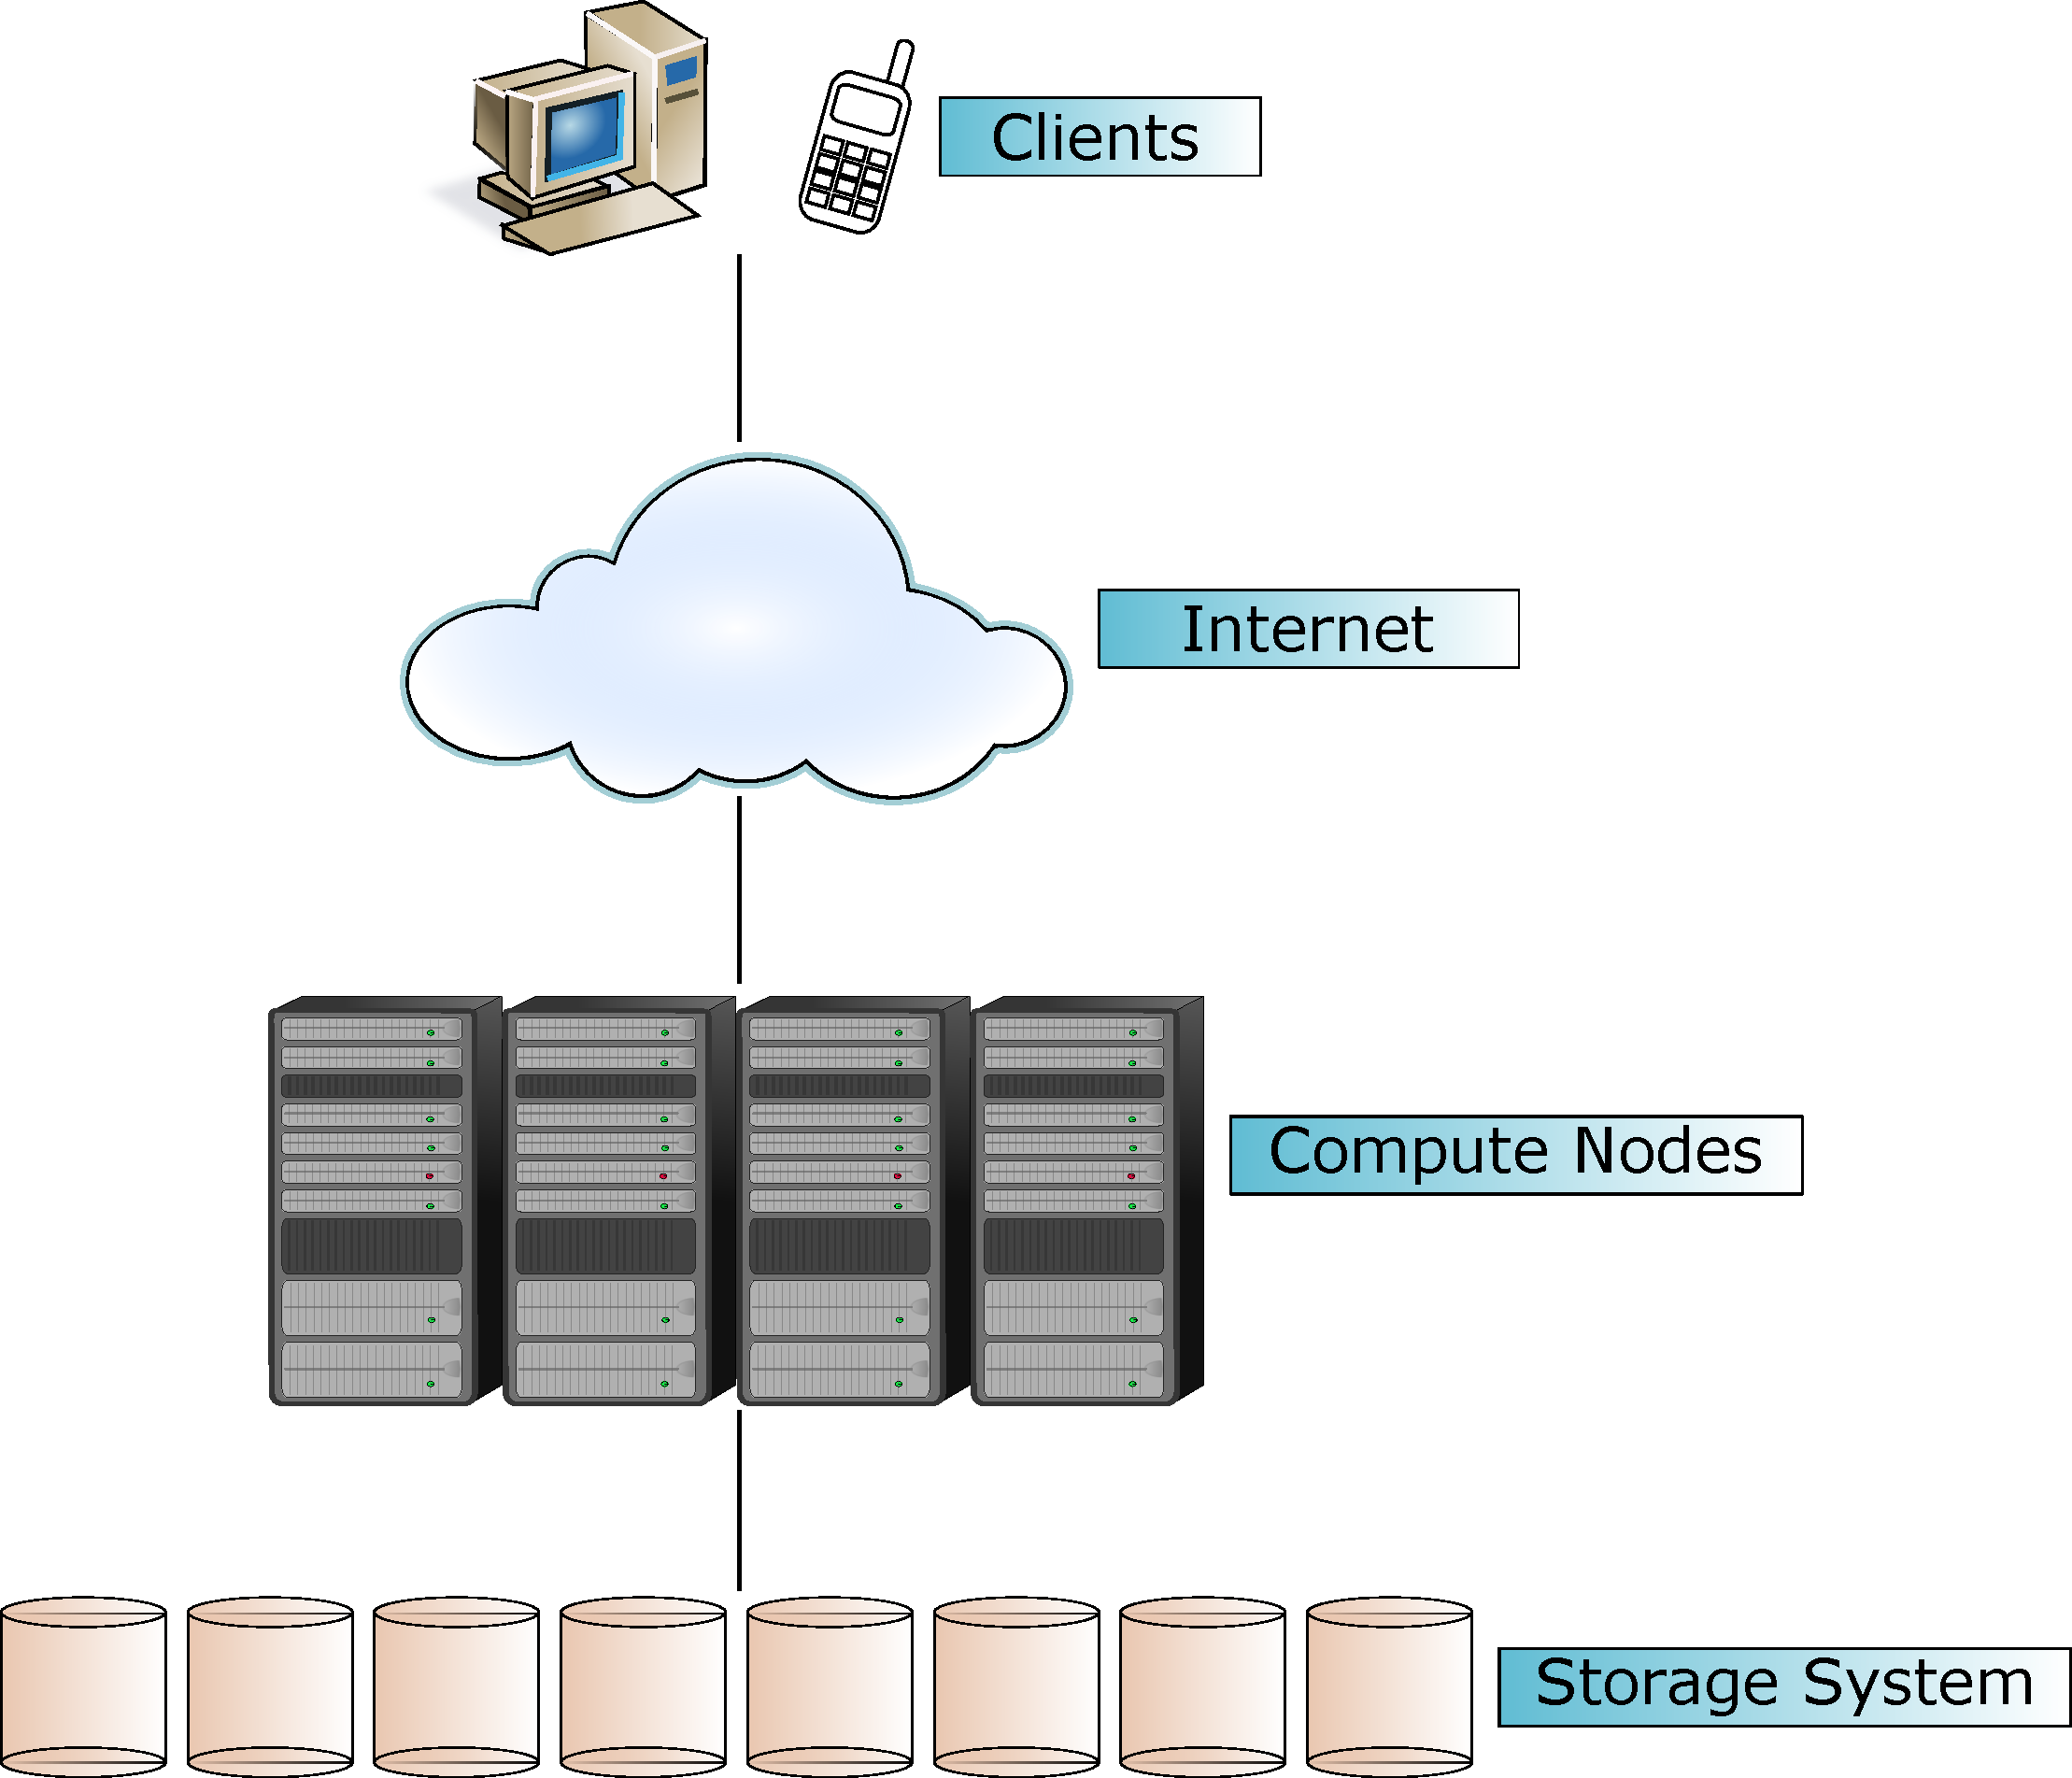
\includegraphics[width=\columnwidth,keepaspectratio]{FIG1.pdf}
\caption{Typical cloud system architecture}
\label{fig:cloud_architecture}
\end{figure}

% XXX Before talking about incasting explain the traditional structure
% XXX of a parallel storage system - e.g. a SAN with parallel storage
% XXX nodes connected through a switch with cloud compute nodes.  A
% XXX reference to the earlier figure might be useful
\textit{Incasting} is a condition that occurs because of queue limitations in most network
switches~\cite{Nagle:2004:PAS:1048933.1049998}. As a result of the incasting behavior, there
is a limit to the number of storage nodes (e.g. 4 servers in a cluster-based storage network
as in~\cite{Krevat:2007:AAA:1374596.1374598}) across which data can be
striped for parallel access. Beyond this limit,
the I/O bandwidth no longer scales and in fact deteriorates. If $M$ represents the number of nodes at
which the performance maxes out, from a performance point of view, there is no point in using more
than $M$ nodes to increase parallelism. While for performance scaling, we would only need $M$ storage nodes in the system,
however, for storage capacity reasons, we may need more than $M$ nodes. In such systems, we would
need to keep these extra nodes active and thus waste energy since the network resources are maxed-out
by a \textit{subset} (of size $M$) of the storage nodes.

To save energy, one could turn off these extra storage nodes, and activate them when necessary. The
difficulty comes while trying to identify which storage nodes should be turned on or off. Our approach
is to distribute cloud users across the storage nodes, such that each user is allocated only $M$
nodes - i.e. the limit at which performance is maxed out. Grouping data on a subset of the storage nodes
and putting the remaining nodes into low power modes has been studied in many related
studies~\cite{Kaushik:2010:GTE:1924920.1924927, Kaushik:2010:LSE:1851476.1851523, Leverich:2010:EEH:1740390.1740405}.
However, the majority of these studies used data classifications,
redundant data or a hot-cold zone approach
to group data on a subset of the storage nodes. Our approach is different from existing studies in that
we try to group \textit{cloud users} on a subset of the storage nodes without any data classification. Not
classifying data enables our methods to be implemented in cloud storage systems with any kind of
redundancy scheme. It is important to also note that, because of the job processing structure (batch mode or
intelligent schedulers) in clouds, we can effectively turn on and off storage nodes based on the user job
submissions since we know a priori which $M$ nodes are going to be used at any time. Therefore, any latency
due to transitioning a storage node from inactive to active mode can be hidden. 

The challenge becomes now how to allocate a subset of cloud storage nodes for each user in order to reduce 
the energy footprint, while at the same time trying to preserve uniform distribution of the system resources if
demanded. We exploit the heterogeneity in the user metadata for energy-aware storage node allocation. As an
example, if we assume a storage system consists of $N$ storage nodes and $M$ of them
max out the incast bandwidth ($N > M$), then each user can be assigned a separate subset of $M$ storage
nodes based on a certain metadata (i.e. user id, usage pattern) and any storage node that is not allocated
for any user at that time can be switched into a low power mode. In this paper, we present several methods
to map subsets of storage nodes to different cloud users and show their outcomes with extensive simulations
using real-world workloads. These approaches build extensively on preliminary methods we presented in our
earlier work~\cite{6322247}.

The rest of this paper is organized as follows: 
Section~\ref{related} gives a brief overview of the related studies. 
Section~\ref{methods} describes the implementation of the node allocation methods we are proposing.
Section~\ref{model} presents a mathematical model to estimate the outcomes of the proposed methods.
Section~\ref{theory} evaluates the proposed methods theoretically to show their approximation factors
to the optimal solutions.
Section~\ref{results} gives the experimental evaluation results of the proposed node allocation methods
and validates the mathematical model proposed in Section~\ref{model}.
Finally, we present conclusions and possible future work in Section~\ref{conclusion}.

Cloud systems have gained popularity over the last decade by enabling users to store data, host
applications and perform computations over the network. Cloud systems significantly decrease
the cost on the user end as management, maintenance and administration tasks are typically
handled by the cloud providers. Cloud providers also benefit from this scheme as they can
utilize system resources more efficiently through techniques, such as virtualization, enabling them
to achieve better performance and energy efficiency. There are numerous cloud providers
offering a broad range of services~\cite{googlece, aws, azure}.

Even though cloud systems tend to have lower energy costs compared to traditional HPC clusters
due to better utilization techniques, the increasing energy consumption of cloud systems still
needs to be addressed as the amount of data stored and the number of computations and applications
in cloud increase steadily. According to \cite{Kaushik:2010:LSE:1851476.1851523}, the estimated
energy consumption of U.S. data centers was more than 100 billion Kilowatt hours in 2011.
Between 2005 and 2010, data centers consumed between 1.7\% and 2.2\% of all electricity in the
U.S.~\cite{koomey2011growth}, matching the energy consumption of the aviation industry.
Increasing energy consumption also means higher cooling costs and additionally, a cloud system with an
underperforming cooling mechanism may have reliability issues potentially causing violations of
service-level agreements (SLA) with the cloud users. It is, therefore, very important to have an
energy-efficient cloud system not only for lower energy costs, but to also meet performance
demands of the cloud users as well.

A typical cloud system is shown in Figure~\ref{fig:cloud_architecture}. In this work, we refer to any 
application using the backend storage of a cloud system as the \textit{user} of that storage system.
There are several components in a cloud system contributing to the overall energy consumption - namely
 processing units, network
components and storage systems. In this work, we specifically target the energy consumption of the
cloud storage infrastructure forming the backend of the cloud computing units, since the storage
system costs constitute an important fraction (between 25-35\%) of overall cloud system
costs~\cite{Harnik:2009:LPM:1586640.1587438, Kim:2011:EPD:1951365.1951378, netapp_power}. Storage
systems also have more idle periods since data stored is usually redundant and archival, written once
and not touched again~\cite{Miller93}. There have been many studies to reduce the energy consumption of
other components of cloud systems. However, since idleness is not usually available in the network
and processing units of clouds, these studies have been mostly on virtual machine consolidation,
workload characterization, data migration or scheduling. In this work, we propose methods to have
an energy-aware cloud storage system while at the same time trying to achieve uniform system
utilization on demand. In particular, we take advantage of idleness existing in cloud storage systems
and try to switch inactive nodes into low power modes. Our work is driven by two key assumptions: first,
the cloud storage system suffers from incasting, and second, most of the data stored in the cloud (as much
as 75\%) is not heavily accessed~\cite{netapp_power}, creating idle periods. It is
important to note that our methods can also be implemented in the storage systems that form the backend
of computational platforms (i.e. Hadoop clusters), where there might be idle
periods~\cite{Kaushik:2010:GTE:1924920.1924927, Narayanan:2008:WOP:1416944.1416949}.


\begin{figure}[!htbp]
\centering
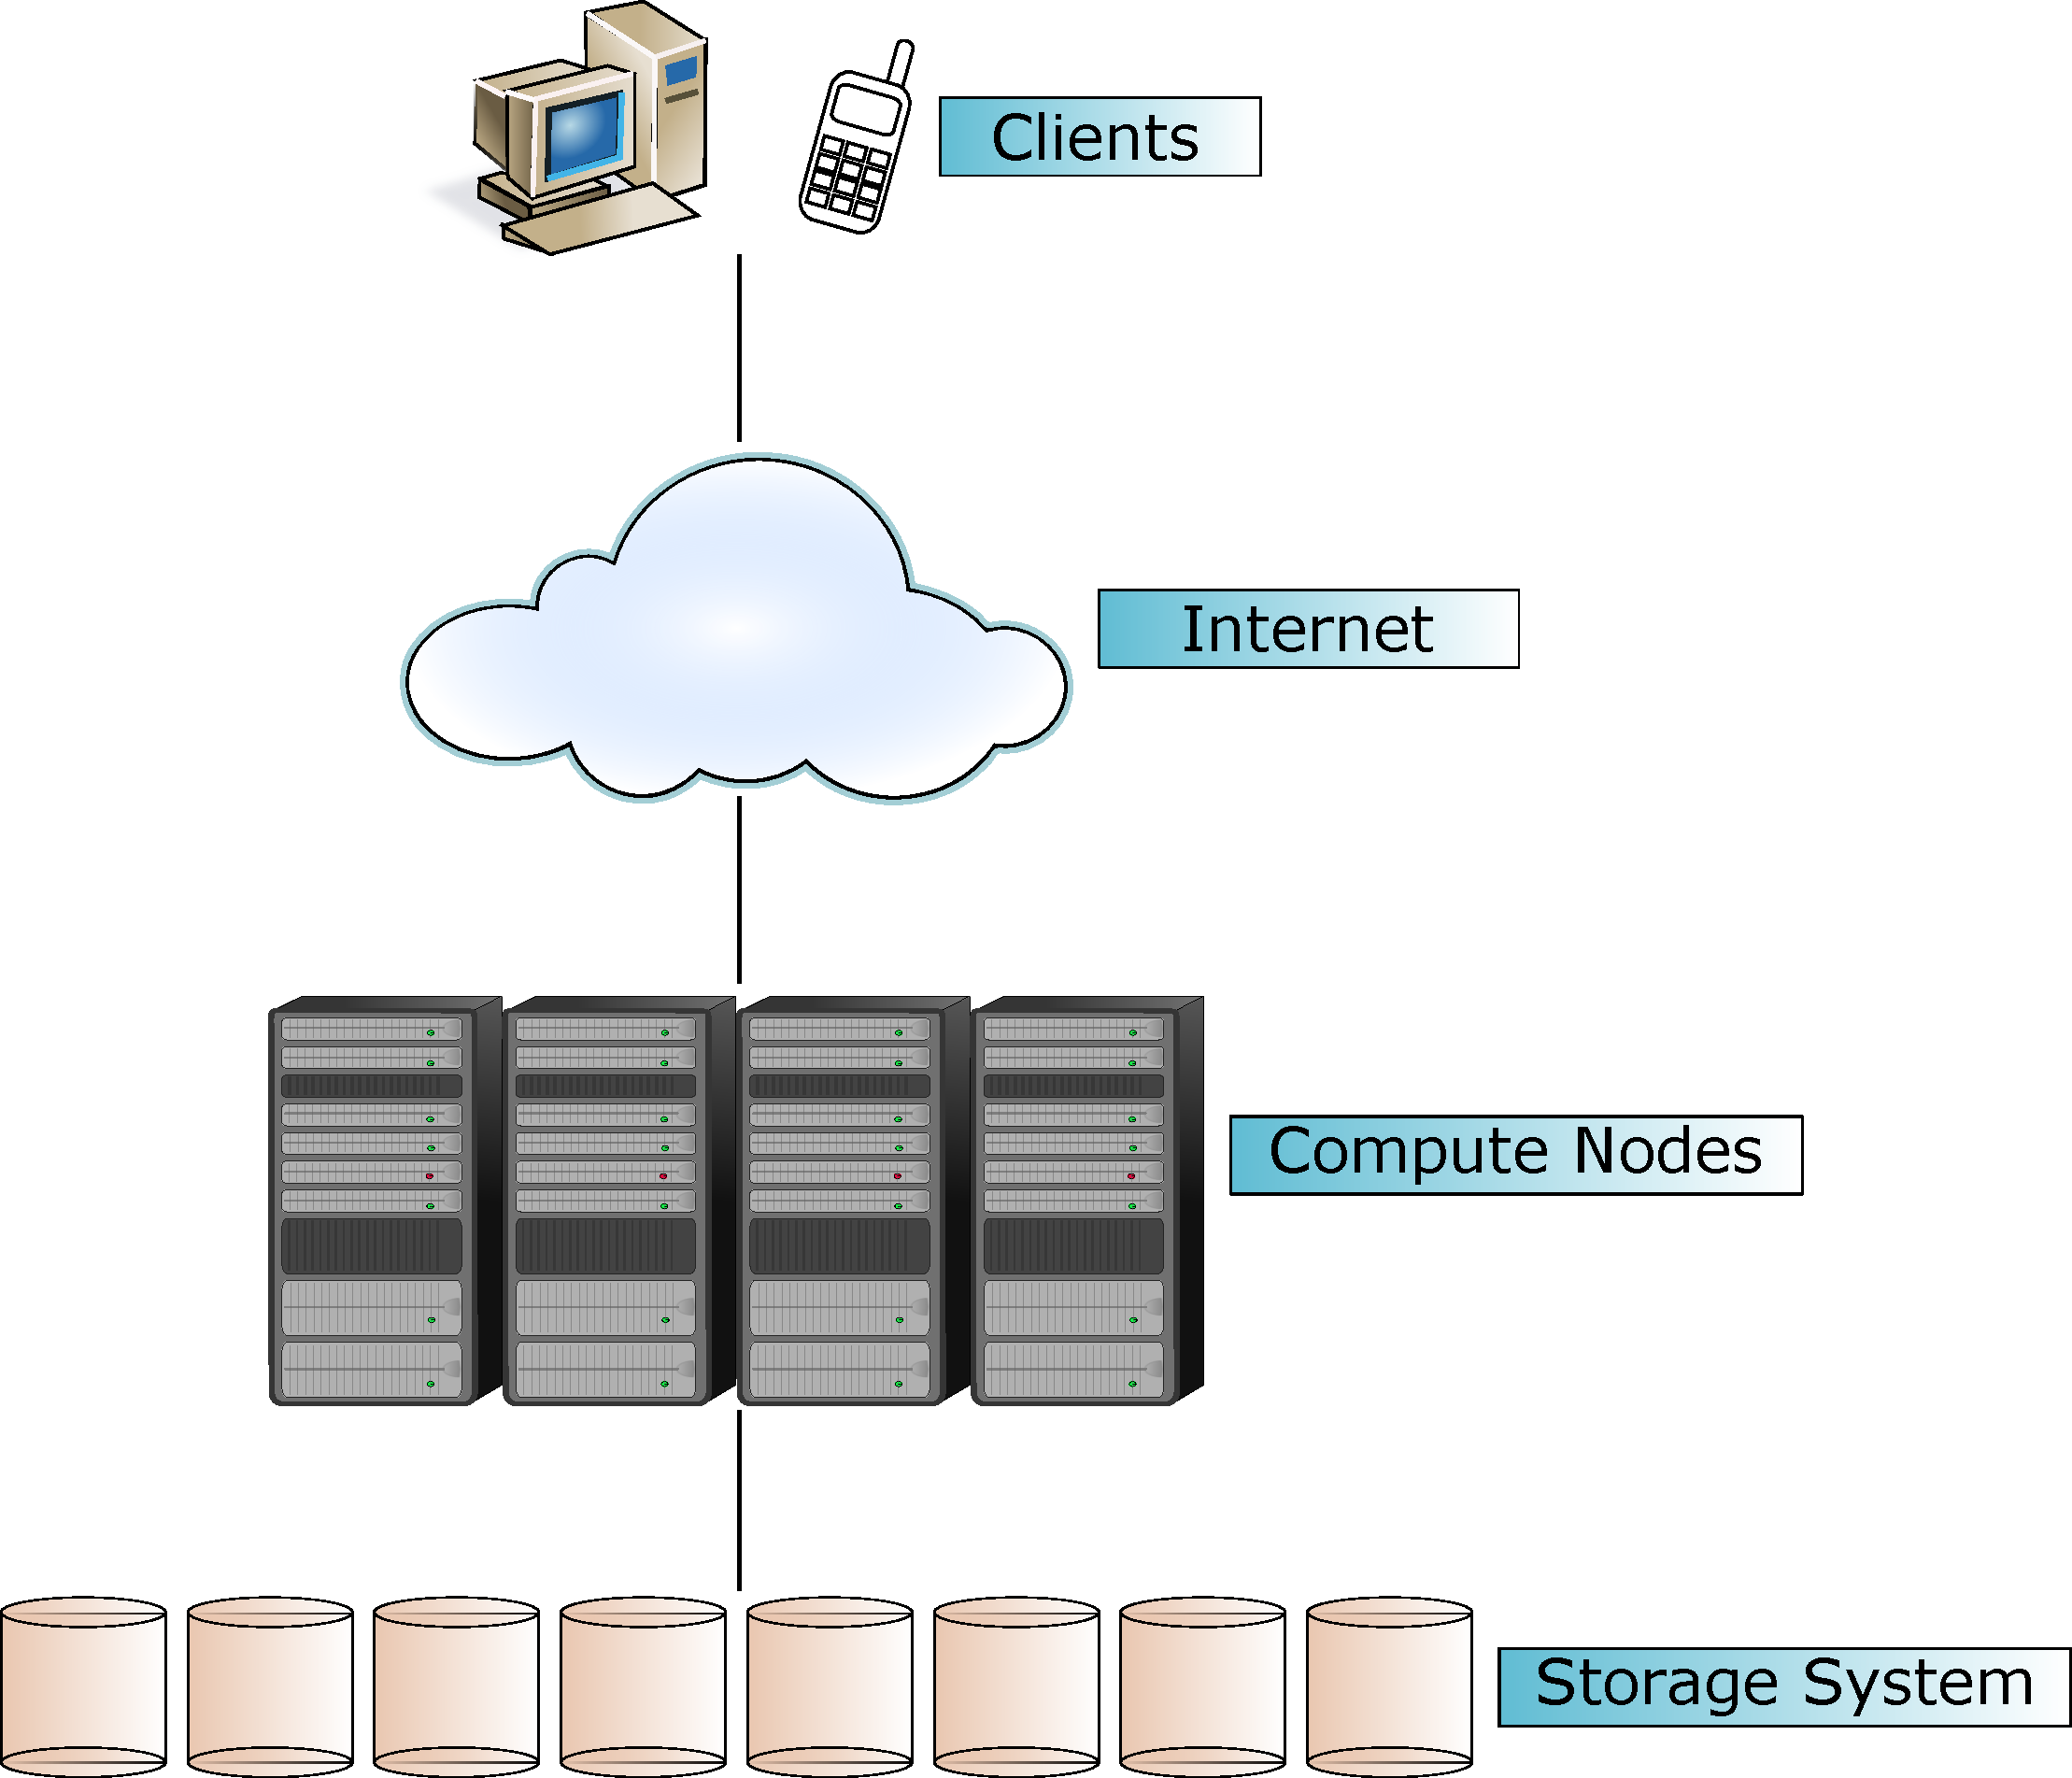
\includegraphics[width=\columnwidth,keepaspectratio]{FIG1.pdf}
\caption{Typical cloud system architecture}
\label{fig:cloud_architecture}
\end{figure}

\textit{Incasting} is a condition that occurs because of queue limitations in most network
switches~\cite{Nagle:2004:PAS:1048933.1049998}. As a result of the incasting behavior, there
is a limit to the number of storage nodes (e.g. 4 servers in a cluster-based storage network
as in~\cite{Krevat:2007:AAA:1374596.1374598}) across which data can be
striped for parallel access. Beyond this limit,
the I/O bandwidth no longer scales and in fact deteriorates. If $M$ represents the number of nodes at
which the performance maxes out, from a performance point of view, there is no point in using more
than $M$ nodes to increase parallelism. While for performance scaling, we would only need $M$ storage nodes in the system,
however, for storage capacity reasons, we may need more than $M$ nodes. In such systems, we would
need to keep these extra nodes active and thus waste energy since the network resources are maxed-out
by a \textit{subset} (of size $M$) of the storage nodes.

To save energy, one could turn off these extra storage nodes, and activate them when necessary. The
difficulty comes while trying to identify which storage nodes should be turned on or off. Our approach
is to distribute cloud users across the storage nodes, such that each user is allocated only $M$
nodes - i.e. the limit at which performance is maxed out. Grouping data on a subset of the storage nodes
and putting the remaining nodes into low power modes has been studied in many related
studies~\cite{Kaushik:2010:GTE:1924920.1924927, Kaushik:2010:LSE:1851476.1851523, Leverich:2010:EEH:1740390.1740405}.
However, the majority of these studies used data classifications,
redundant data or a hot-cold zone approach
to group data on a subset of the storage nodes. Our approach is different from existing studies in that
we try to group \textit{cloud users} on a subset of the storage nodes without any data classification. Not
classifying data enables our methods to be implemented in cloud storage systems with any kind of
redundancy scheme. It is important to also note that, because of the job processing structure (batch mode or
intelligent schedulers) in clouds, we can effectively turn on and off storage nodes based on the user job
submissions since we know a priori which $M$ nodes are going to be used at any time. Therefore, any latency
due to transitioning a storage node from inactive to active mode can be hidden. 

The challenge becomes now how to allocate a subset of cloud storage nodes for each user in order to reduce 
the energy footprint, while at the same time trying to preserve uniform distribution of the system resources if
demanded. We exploit the heterogeneity in the user metadata for energy-aware storage node allocation. As an
example, if we assume a storage system consists of $N$ storage nodes and $M$ of them
max out the incast bandwidth ($N > M$), then each user can be assigned a separate subset of $M$ storage
nodes based on a certain metadata (i.e. user id, usage pattern) and any storage node that is not allocated
for any user at that time can be switched into a low power mode. In this paper, we present several methods
to map subsets of storage nodes to different cloud users and show their outcomes with extensive simulations
using real-world workloads. These approaches build extensively on preliminary methods we presented in our
earlier work~\cite{6322247}.

The rest of this paper is organized as follows: 
Section~\ref{related} gives a brief overview of the related studies. 
Section~\ref{methods} describes the implementation of the node allocation methods we are proposing.
Section~\ref{model} presents a mathematical model to estimate the outcomes of the proposed methods.
Section~\ref{theory} evaluates the proposed methods theoretically to show their approximation factors
to the optimal solutions.
Section~\ref{results} gives the experimental evaluation results of the proposed node allocation methods
and validates the mathematical model proposed in Section~\ref{model}.
Finally, we present conclusions and possible future work in Section~\ref{conclusion}.

\section{Related Work}
\label{related}
%%The energy consumption of cloud systems has been studied extensively by the research
community. Srikantaiah et al. reduce the energy consumption of cloud systems
with workload consolidation while trying to find optimal performance
energy trade-off points~\cite{Srikantaiah:2008:EAC:1855610.1855620}.
In \cite{Kim:2009:PPC:1657120.1657121}, authors present energy aware provisioning
of virtual machines in a cloud system. Harnik et al. investigate how cloud storage
systems can operate at low-power modes while maximizing data availability and the
number of nodes to power down~\cite{Harnik:2009:LPM:1586640.1587438}. Duy et al.
propose a green scheduling algorithm to predict the future load in a cloud
system and to turn off unused nodes~\cite{5470908}. CloudScale reserves resources
based on usage in a multi-tenant cloud to reduce energy consumption~\cite{Shen:2011:CER:2038916.2038921}.
Rabbit is a distributed file system trying to save energy by turning off nodes while
making sure that at least primary data replicas are available~\cite{Amur:2010:RFP:1807128.1807164}.
Beloglazov et al. present a model to detect an overloaded host and dynamically reallocate
the virtual machines on that host for improved energy efficiency and
performance~\cite{Beloglazov:2013:MOH:2498743.2498939}

There also have been numerous studies to reduce the energy consumption of storage
and file systems in general. Most existing energy saving techniques for these systems
attempt to move less frequently used data to a subset of the nodes. Massive Array of Idle
Disks~\cite{Colarelli:2002:MAI:762761.762819} (MAID) forms two groups of storage nodes in the
system - \textit{active} and \textit{passive}. New requests are typically handled by the active
nodes, and if not, they are forwarded to the passive nodes. MAID's performance, however, is
dependent on the workload and cache characteristics.
Popular Data Concentration~\cite{Pinheiro:2004:ECT:1006209.1006220} (PDC) is another similar
technique where frequently accessed data is migrated to a group of storage nodes, called
\textit{active} nodes. Before migrating data, PDC needs to predict the future load for each storage
node. Although performing better than MAID for small workloads, PDC suffers from the overhead of
data migration and load prediction.
Wildani et al. present a technique that identifies and brings together data blocks in a workload
for better energy management, based on the likelihood of related access~\cite{Wildani:2011:EIW:1987816.1987823}.
GreenHDFS uses a hot\&cold zone approach, where frequently accessed data is located on the storage
nodes in the hot zone and unpopular data is located on the storage nodes in the cold
zone~\cite{Kaushik:2010:GTE:1924920.1924927}.
Lightning is an energy-aware cloud storage system that divides the storage nodes into hot\&cold zones
with data-classification driven data placement~\cite{Kaushik:2010:LSE:1851476.1851523}. The purpose of dividing
the storage nodes into logical hot\&cold zones is to increase the idleness in the storage system.
There have been other relevant studies that aimed directly at making better use of idle periods in a storage system.
Mountroidou et al. presents a framework that identifies when and for how long to activate a power-saving
mode to meet given performance\&power constraints~\cite{10.1109/IGCC.2011.6008570}. They also propose adaptive
workload shaping to make use of the idle periods in a workload better~\cite{Mountrouidou:2011:AWS:1958746.1958766}.
Write-offloading technique shows that enterprise workloads have idle periods as well and these periods
can be increased further by offloading writes on spun-down disks to persistent storage~\cite{Narayanan:2008:WOP:1416944.1416949}.
SRCMap is another technique where the workload is selectively consolidated on a subset of storage
nodes, proportional to the I/O workload~\cite{Verma:2010:SEP:1855511.1855531}. These data-classification driven
placement techniques work well only if one is able to predict data usage and idle period with reasonable
accuracy.

Hardware based techniques can also help with energy utilization but is
not broadly applicable.
Barroso et al. proposed that server components, particularly memory and disk
subsystems, need improvements to consume power proportional to their utilization levels~\cite{33387}.
Hibernator uses disks that can operate at different speeds to reduce energy consumption while trying to
meet performance goals~\cite{Zhu:2005:HHD:1095810.1095828}.

Architectural or file system optimizations present another opportunity
to save energy.
Ganesh et al.~\cite{GaneshWeatherspoonBalakrishnanBirman07_OptimizingPowerConsumptionInLargeScaleStorageSystems}
has shown that the Log Structured Filesystem (LFS) can be used to reduce energy consumption, since
the write requests are recorded in a log file making it possible to know on the client side which
storage node will handle the write request. This approach suffers from the overhead of cleaning
the log file.
Leverich and Kozyrakis present a technique to reduce the energy consumption of Hadoop clusters using
covering subsets to ensure data availability~\cite{Leverich:2010:EEH:1740390.1740405}. They find a trade-off
between energy savings and overall performance of the system.
Pergamum is a distributed archival storage system that saves energy by avoiding centralized controllers
~\cite{Storer:2008:PRT:1364813.1364814}.
Zhu et al. proposes power-aware storage cache management algorithms to keep the disks in low-power modes
for longer~\cite{Zhu:2004:REC:1072448.1072462}.
Diverted Access is another technique that exploits the redundancy in the storage systems to reduce
energy consumption~\cite{Pinheiro:2006:ERC:1140277.1140281}.

In more recent related studies, Chen et al. present the \textit{k-out-of-n computing} framework~\cite{6847230}
with the goal of increasing fault-tolerance and energy-efficiency during storage system access and data
processing. Eventhough, the random and greedy approaches used during the evaluations is similar
to the methods we will propose, this work is tailored for mobile devices in a dynamic network and unlike our
study, it is not concerned with load balancing. In~\cite{Collotta2015137}, the authors propose a fuzzy logic
approach that tries to improve the energy-efficiency of Bluetooth Low Energy (BLE) network used in many
Internet-of-Things environments, by predicting sleeping periods of devices in BLE network using their battery
levels and throughput-to-workload ratios. Eventhough, the scope and parameters of this work is completely
different than our approach, the authors show a method to benefit from idleness in a system using data from
system components. Finally, Sallam et al. present a proactive workload manager that tries to avoid bursty loads and
underutilization of resources that might be caused by a reactive workload manager in a virtual environment~\cite{Sallam:2014:PWM:2658292.2658555}.
They proactively predict the future state of VMs by analyzing the recently observed patterns. This approach
is similar to the future prediction method we will propose in Dynamic Greedy and Correlation-Based schemes; although,
it is tailored for virtual environments.

To the best of our knowledge, there has not been any related study trying to reduce energy consumption in 
a cloud storage system by using user metadata. The most relevant to our work is the approach by Wildani et al.
to group semantically-related data across the same set of devices to reduce the number of disk accesses resulting
in disk spin-ups. However, they group related data, while we group related users together~\cite{5668053}.


The energy consumption of cloud systems has been studied extensively by the research
community. Srikantaiah et al. reduce the energy consumption of cloud systems
with workload consolidation while trying to find optimal performance
energy trade-off points~\cite{Srikantaiah:2008:EAC:1855610.1855620}.
In \cite{Kim:2009:PPC:1657120.1657121}, authors present energy aware provisioning
of virtual machines in a cloud system. Harnik et al. investigate how cloud storage
systems can operate at low-power modes while maximizing data availability and the
number of nodes to power down~\cite{Harnik:2009:LPM:1586640.1587438}. Duy et al.
propose a green scheduling algorithm to predict the future load in a cloud
system and to turn off unused nodes~\cite{5470908}. CloudScale reserves resources
based on usage in a multi-tenant cloud to reduce energy consumption~\cite{Shen:2011:CER:2038916.2038921}.
Rabbit is a distributed file system trying to save energy by turning off nodes while
making sure that at least primary data replicas are available~\cite{Amur:2010:RFP:1807128.1807164}.
Beloglazov et al. present a model to detect an overloaded host and dynamically reallocate
the virtual machines on that host for improved energy efficiency and
performance~\cite{Beloglazov:2013:MOH:2498743.2498939}

There also have been numerous studies to reduce the energy consumption of storage
and file systems in general. Most existing energy saving techniques for these systems
attempt to move less frequently used data to a subset of the nodes. Massive Array of Idle
Disks~\cite{Colarelli:2002:MAI:762761.762819} (MAID) forms two groups of storage nodes in the
system - \textit{active} and \textit{passive}. New requests are typically handled by the active
nodes, and if not, they are forwarded to the passive nodes. MAID's performance, however, is
dependent on the workload and cache characteristics.
Popular Data Concentration~\cite{Pinheiro:2004:ECT:1006209.1006220} (PDC) is another similar
technique where frequently accessed data is migrated to a group of storage nodes, called
\textit{active} nodes. Before migrating data, PDC needs to predict the future load for each storage
node. Although performing better than MAID for small workloads, PDC suffers from the overhead of
data migration and load prediction.
Wildani et al. present a technique that identifies and brings together data blocks in a workload
for better energy management, based on the likelihood of related access~\cite{Wildani:2011:EIW:1987816.1987823}.
GreenHDFS uses a hot\&cold zone approach, where frequently accessed data is located on the storage
nodes in the hot zone and unpopular data is located on the storage nodes in the cold
zone~\cite{Kaushik:2010:GTE:1924920.1924927}.
Lightning is an energy-aware cloud storage system that divides the storage nodes into hot\&cold zones
with data-classification driven data placement~\cite{Kaushik:2010:LSE:1851476.1851523}. The purpose of dividing
the storage nodes into logical hot\&cold zones is to increase the idleness in the storage system.
There have been other relevant studies that aimed directly at making better use of idle periods in a storage system.
Mountroidou et al. presents a framework that identifies when and for how long to activate a power-saving
mode to meet given performance\&power constraints~\cite{10.1109/IGCC.2011.6008570}. They also propose adaptive
workload shaping to make use of the idle periods in a workload better~\cite{Mountrouidou:2011:AWS:1958746.1958766}.
Write-offloading technique shows that enterprise workloads have idle periods as well and these periods
can be increased further by offloading writes on spun-down disks to persistent storage~\cite{Narayanan:2008:WOP:1416944.1416949}.
SRCMap is another technique where the workload is selectively consolidated on a subset of storage
nodes, proportional to the I/O workload~\cite{Verma:2010:SEP:1855511.1855531}. These data-classification driven
placement techniques work well only if one is able to predict data usage and idle period with reasonable
accuracy.

Hardware based techniques can also help with energy utilization but is
not broadly applicable.
Barroso et al. proposed that server components, particularly memory and disk
subsystems, need improvements to consume power proportional to their utilization levels~\cite{33387}.
Hibernator uses disks that can operate at different speeds to reduce energy consumption while trying to
meet performance goals~\cite{Zhu:2005:HHD:1095810.1095828}.

Architectural or file system optimizations present another opportunity
to save energy.
Ganesh et al.~\cite{GaneshWeatherspoonBalakrishnanBirman07_OptimizingPowerConsumptionInLargeScaleStorageSystems}
has shown that the Log Structured Filesystem (LFS) can be used to reduce energy consumption, since
the write requests are recorded in a log file making it possible to know on the client side which
storage node will handle the write request. This approach suffers from the overhead of cleaning
the log file.
Leverich and Kozyrakis present a technique to reduce the energy consumption of Hadoop clusters using
covering subsets to ensure data availability~\cite{Leverich:2010:EEH:1740390.1740405}. They find a trade-off
between energy savings and overall performance of the system.
Pergamum is a distributed archival storage system that saves energy by avoiding centralized controllers
~\cite{Storer:2008:PRT:1364813.1364814}.
Zhu et al. proposes power-aware storage cache management algorithms to keep the disks in low-power modes
for longer~\cite{Zhu:2004:REC:1072448.1072462}.
Diverted Access is another technique that exploits the redundancy in the storage systems to reduce
energy consumption~\cite{Pinheiro:2006:ERC:1140277.1140281}.

In more recent related studies, Chen et al. present the \textit{k-out-of-n computing} framework~\cite{6847230}
with the goal of increasing fault-tolerance and energy-efficiency during storage system access and data
processing. Eventhough, the random and greedy approaches used during the evaluations is similar
to the methods we will propose, this work is tailored for mobile devices in a dynamic network and unlike our
study, it is not concerned with load balancing. In~\cite{Collotta2015137}, the authors propose a fuzzy logic
approach that tries to improve the energy-efficiency of Bluetooth Low Energy (BLE) network used in many
Internet-of-Things environments, by predicting sleeping periods of devices in BLE network using their battery
levels and throughput-to-workload ratios. Eventhough, the scope and parameters of this work is completely
different than our approach, the authors show a method to benefit from idleness in a system using data from
system components. Finally, Sallam et al. present a proactive workload manager that tries to avoid bursty loads and
underutilization of resources that might be caused by a reactive workload manager in a virtual environment~\cite{Sallam:2014:PWM:2658292.2658555}.
They proactively predict the future state of VMs by analyzing the recently observed patterns. This approach
is similar to the future prediction method we will propose in Dynamic Greedy and Correlation-Based schemes; although,
it is tailored for virtual environments.

To the best of our knowledge, there has not been any related study trying to reduce energy consumption in 
a cloud storage system by using user metadata. The most relevant to our work is the approach by Wildani et al.
to group semantically-related data across the same set of devices to reduce the number of disk accesses resulting
in disk spin-ups. However, they group related data, while we group related users together~\cite{5668053}.


\section{Proposed Techniques}
\label{methods}
%%In order to tackle the energy efficiency problem of cloud storage systems, we propose
allocating nodes for each user based on the metadata information of that user
and switch the inactive nodes to low energy modes. As described earlier, we assume
a use scenario where a subset of the storage nodes max out the
available bandwidth of the system due to incasting. Therefore, it is not feasible to allocate more
than $M$ nodes to each user both for performance and energy efficiency reasons. Here $M$
represents the number of storage nodes in a subset allocated for a user. Therefore,
the problem we are trying to solve is how to map subsets of the storage nodes to the users.
Since user metadata heterogeneity is well-defined in large-scale cloud systems, we
retrieve user metadata information (i.e. user id, usage pattern) and
allocate subsets of storage nodes to the users using this information.

In this work, we propose three different methods to map cloud storage nodes to the
cloud users, summarized as follows:

\begin{itemize}
\item \textit{Fixed Scheme}: There
are four node allocation techniques in this method: \textit{balancing}, \textit{sequential},
\textit{random} and \textit{grouping} and once one of these techniques is chosen for a
cloud storage system, it remains in effect unless manually changed.
\item \textit{Dynamic Greedy Scheme}: This method
extends the \textit{Fixed Scheme} method by periodically doing dynamic reallocation
among one of the four
allocation techniques (\textit{balancing, sequential, random, grouping}) depending
on their costs. The cost of each technique is calculated based on how important it is
for the cloud storage system to save energy or to balance load.
\item \textit{Correlation-Based Scheme}: This method
monitors user activities and tries to allocate the same subset of storage nodes to the
users who tend to use the cloud storage system concurrently.
\end{itemize}

The energy-aware node allocation methods proposed here are designed to work for a traditional
distributed storage system architecture, but they could also work in a disk array. The
proposed methods not only reduce energy consumption, but also balance load on storage
nodes depending on metrics selected by the cloud administrators.

Before describing each node allocation method in more detail, we first list some of the usage
assumptions in our system and then explain two common
features of the node allocation methods: \textit{inactivity threshold} and \textit{job overlapping}.

We assume that;
\begin{itemize}
\item All storage nodes are initially off and a storage node is started up as soon as a
job arrives.
\item A user uses the same amount of storage space on each of its allocated nodes.
\item Any job run by a user is divided into equal tasks on the nodes allocated for
that user and these tasks are executed concurrently, meaning that they start and
complete simultaneously.
\item If a user is transferred from a subset of the storage nodes to another subset of
the storage nodes, this includes transferring only data. Any jobs that were executed
in the old subset of the storage nodes still belong to those nodes.
\end{itemize}

\paragraph{Inactivity Threshold}
The node allocation methods we are proposing try to save as much energy as possible and
also balance the load on storage nodes depending on metrics selected by the cloud administrators.
If a storage node is not allocated for any user at all, then it will stay in a low-energy mode.
On the other hand, if a storage node is allocated for one or more users, that node will
only switch to a low-energy mode after all jobs using that node are completed.
In an HPC system, the completion time of jobs can be predicted because of job scheduling systems.
Thus, we can decide when to switch a node to a low-energy mode. However, in a cloud storage system,
this predictability is not necessarily always possible, and we need to have a condition to decide when to switch a 
storage node to a low-energy mode. We call this metric the \textit{inactivity threshold}, which
can be defined as \textit{the period of time a node continues to operate at full capacity after the
completion of the most recent storage system job}. This means that, once a node stays inactive for
longer than the inactivity threshold, it can be switched to a
low-energy mode. The \textit{inactivity
threshold}, in this sense, is similar to \textit{break-even time} in previous studies, which ensures
that the energy saved by turning off a node is greater than the energy consumed while switching
that node from active to low-power modes.

In our work, we define the low-energy mode as the state where a node is completely turned off. However,
some modern hard drives have the ability to operate at various
speeds~\cite{Gurumurthi:2003:DDS:871656.859638} thus providing
different levels of energy utilization.
Therefore, in order to conserve energy it is not mandatory to completely turn off a node. Depending on how
much energy saving is demanded by the user, the node allocation techniques can switch nodes into
low-speed operating modes without turning them off. In this work, in order to show the effect of the
node allocation methods better, we assume the worst case and turn off a storage node in low-energy
mode.

If a user is allocated to a node that has been turned off, then that
node needs to start operating at full capacity again. In this case, the user can not immediately access
that storage node, since it will take some time for that node to run at full capacity again. We define the time
it takes to start up a completely turned-off node as the \textit{startup time}. If a storage node has been inactive
between two jobs for longer than the \textit{inactivity threshold}, then the next job on that node
will have to wait for the node to start up.

The \textit{inactivity threshold} and the \textit{startup time} are
important parameters in determining how a real cloud storage
system is going to be affected by the node assignment methods we are proposing.

\paragraph{Job Overlapping}
In a large-scale cloud storage system, each storage node may be used by multiple concurrent users. Our node allocation
methods might allocate a node to multiple users. Therefore, concurrent users can simultaneously
run jobs that use a particular storage node. When two or more jobs overlap on a node, we assume that
node still consumes the same energy per unit
time~\cite{Tsirogiannis:2010:AEE:1807167.1807194}. In other words,
we assume the increased activity due to the multiple jobs will not
increase energy consumption significantly. This is, for the most
part, true because most of the energy is consumed by spinning the
drives not by moving actuators on the drive.

\subsection{Fixed Scheme}
\label{fixed}
In this first scheme, one of the four node allocation techniques described below 
(balancing, sequential, random or grouping) is chosen by the cloud
storage system administrator
and is kept fixed unless manually changed. All techniques have one goal
in common - exploiting user metadata to allocate storage nodes for users. Individually,
each technique performs differently in terms of uniformly allocating storage nodes.
These techniques are each described numerically in Figure~\ref{fixed_examples} with examples.

\begin{figure}[!htbp]
\centering
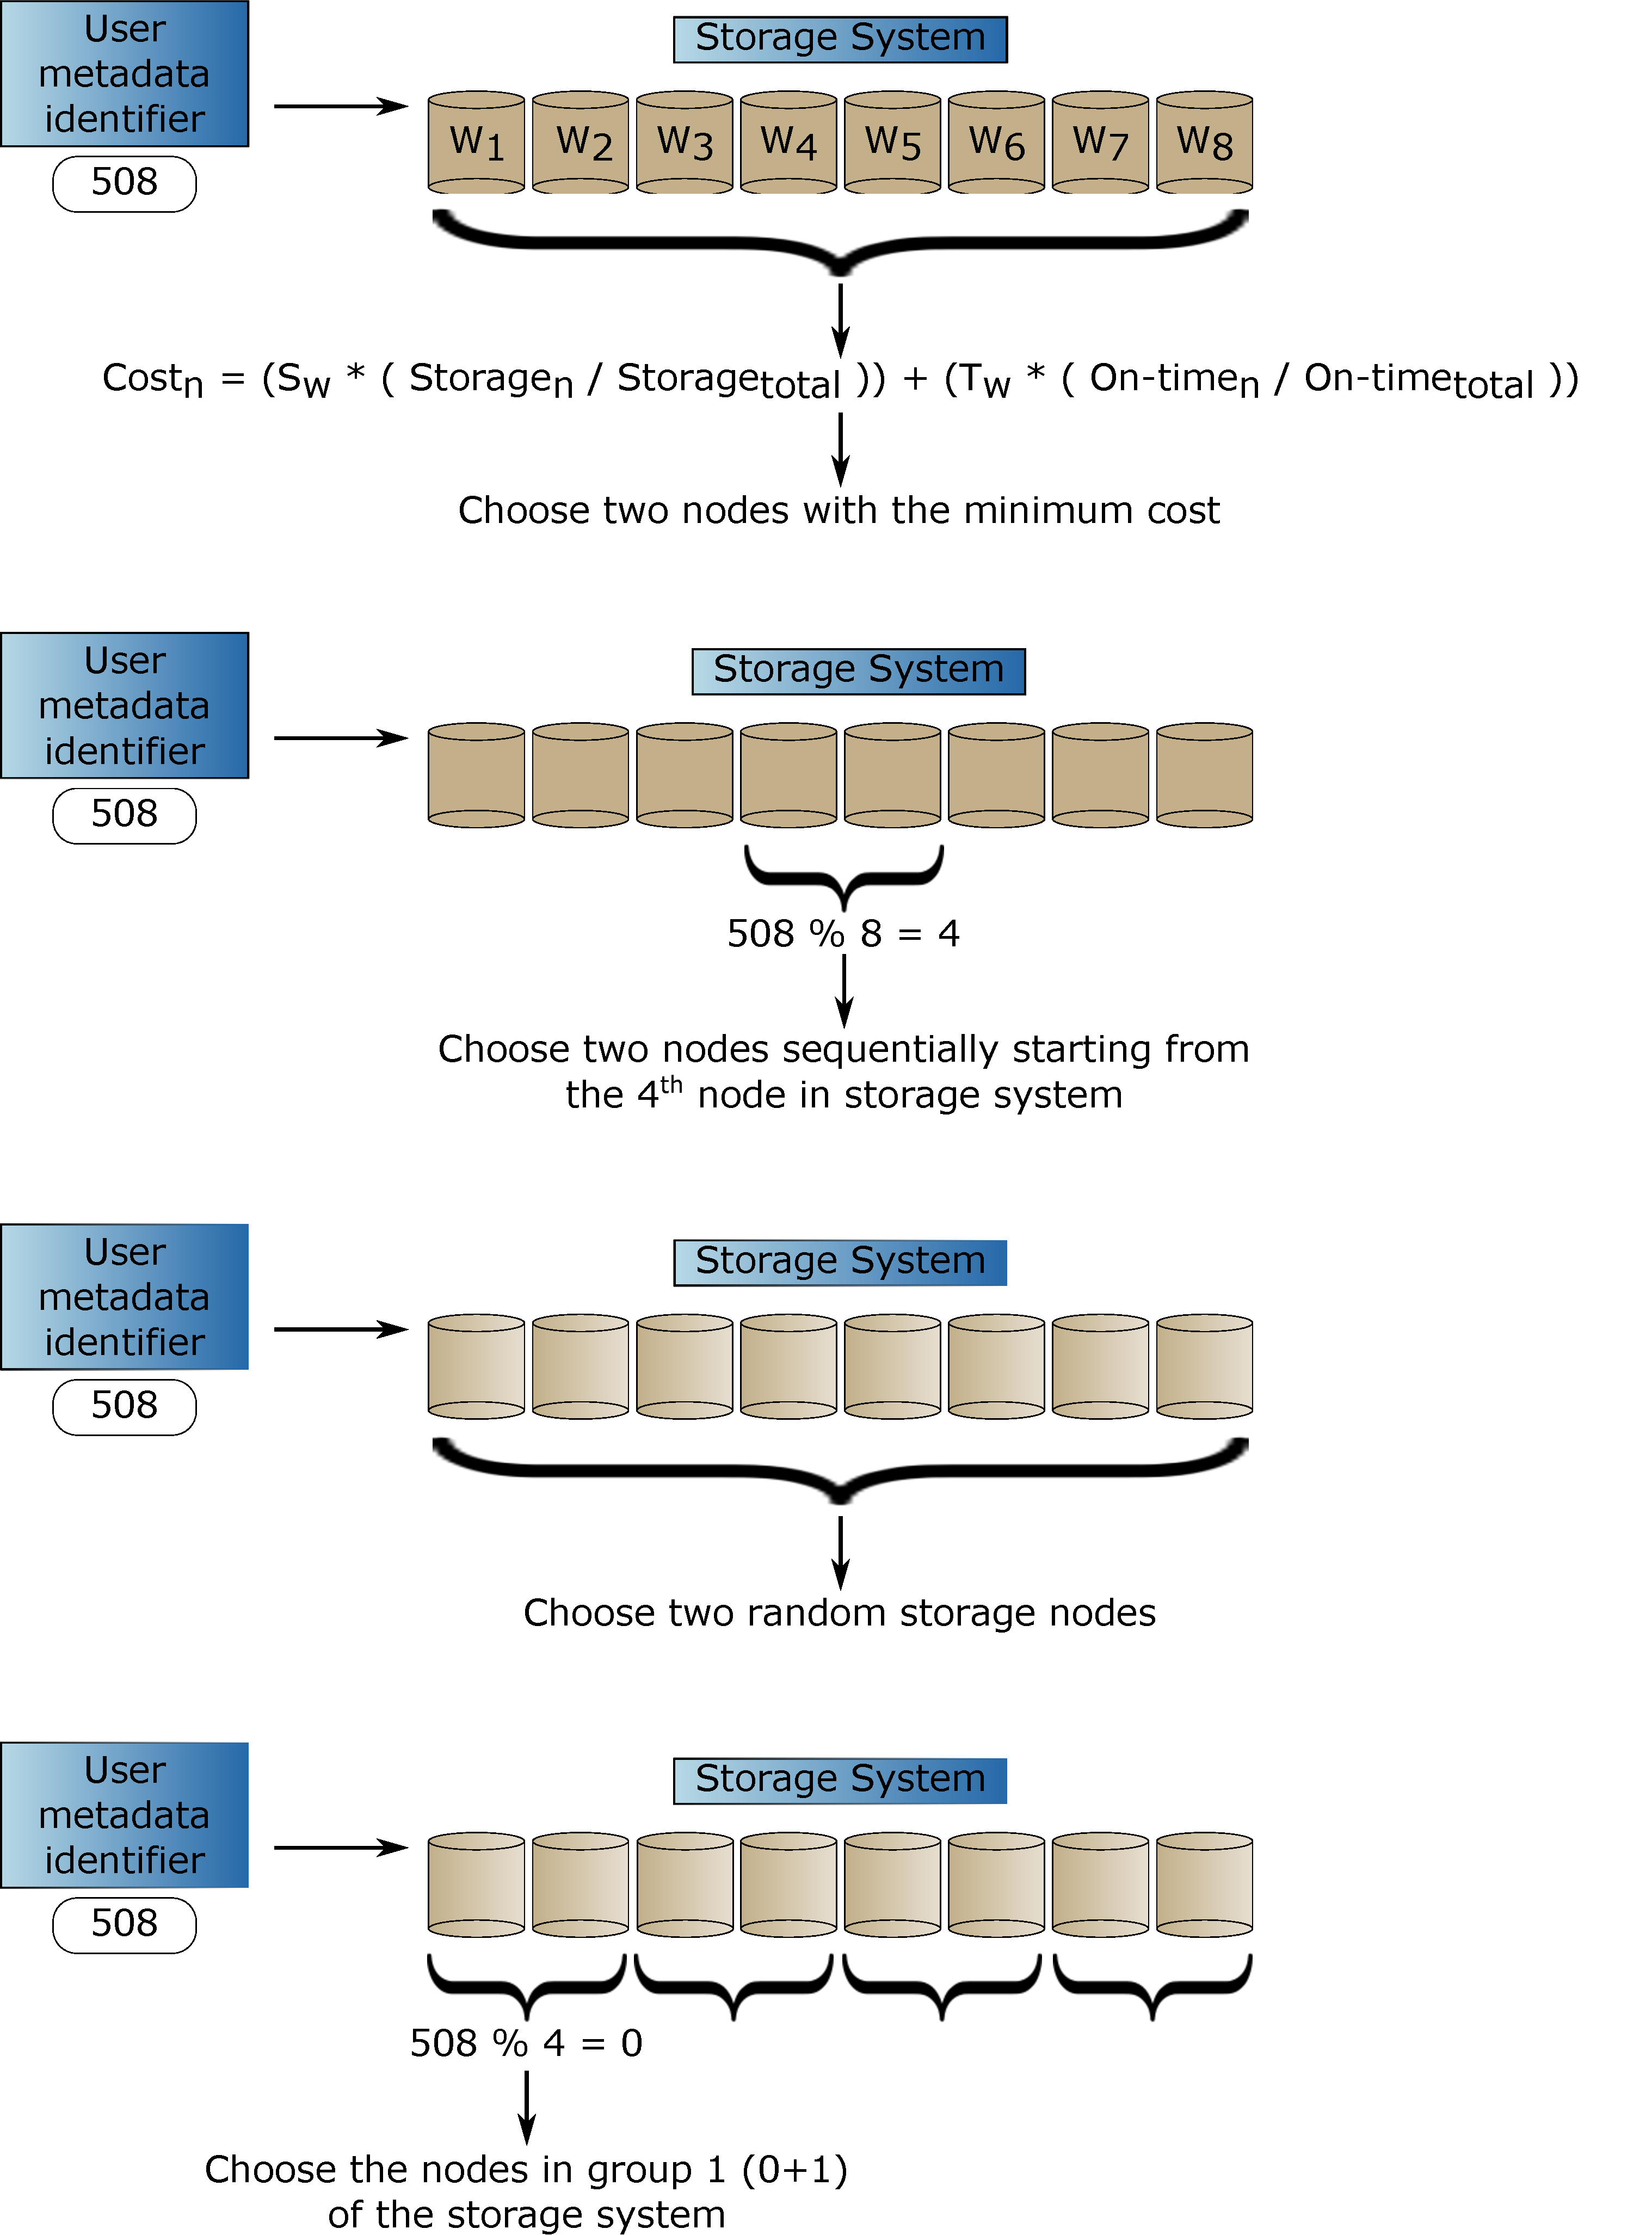
\includegraphics[width=\columnwidth,keepaspectratio]{FIG2.pdf}
\caption{Examples of the node allocation techniques in the Fixed scheme}
\label{fixed_examples}
\end{figure}

\subsubsection{Balancing Technique}
\label{baltechnique}
The primary goal of this technique is to balance the load across the cloud storage nodes. We
define the \textit{load} here in two different ways:

\begin{itemize}
\item The amount of data stored on each node.
\item The total time each node stays on serving user requests.
\end{itemize}

We call balancing the amount of data stored on each node \textit{storage space balancing}.
Similarly, balancing the total time each node stays on is
called \textit{on-time balancing}. These two balancing
techniques ensure that all the nodes in the system are used equally.
Otherwise, the simplest energy saving technique is to simply put all
users and data on the same subset of nodes and permanently turn off
all other nodes. This, however, can cause capacity issues as the
selected nodes may not have enough storage space and also incurs
higher utilization and thus, higher failure rates.
The balancing technique enables system administrators to specify weights for \textit{storage space
balancing} and \textit{on-time balancing} to indicate their importance and allocates
storage nodes for users by adhering to these weights. A \textit{cost} metric is calculated for every
storage node in the system by multiplying storage space and on-time weights with the normalized 
storage space and on-time on that node respectively. In order to normalize storage space and
on-time values, they are divided by the total amount of storage and on-time on all nodes
respectively. In the end, storage nodes with lower costs are preferred by the balancing technique
with the eventual goal of uniformly distributing storage space usage and on-time across storage nodes.
As mentioned previously, we assume the storage space usage of a user is distributed evenly across the
nodes allocated for that user and a job running on multiple nodes concurrently takes the same amount
of time to complete on each node.

Assuming, $N$ is the total number of nodes in the cloud storage system and $M$ is the number
of storage nodes allocated for each user, the balancing technique works as shown in Algorithm~\ref{balapp}.

\begin{algorithm}[!htbp]
\caption{Balancing Technique}
\label{balapp}
\begin{algorithmic}[1]
    \STATE $N \Leftarrow$ Total\ number\ of\ storage\ nodes
    \STATE $M \Leftarrow$ Number\ of\ storage\ nodes\ to\ allocate\ for\ the\ user
    \STATE $ChosenNodes[\ ] \Leftarrow$ Nodes\ that\ will\ be\ allocated\ for\ the\ user
    \STATE $S_{total} \Leftarrow$ Total\ amount\ of\ data\ stored\ on\ all\ nodes
    \STATE $T_{total} \Leftarrow$ Total\ duration\ of\ time\ all\ nodes\ stayed\ on
    \STATE $S_i \Leftarrow$ Amount\ of\ data\ stored\ on\ node\ $i$
    \STATE $T_i \Leftarrow$ Duration\ of\ time\ node\ $i$ stayed\ on
    \STATE $S_W \Leftarrow$ Importance\ of\ balancing\ storage\ space
    \STATE $T_W \Leftarrow$ Importance\ of\ balancing\ time
    \STATE $Costs[\ ] \Leftarrow$ Costs\ of\ nodes\ $i$
    \FOR{$i=1$ to $N$}
        \STATE $Costs[i] \Leftarrow (S_W * (S_i/S_{total}) + (T_W * (T_i/T_{total}))$
    \ENDFOR
    \FOR{$i=1$ to $M$}
        \STATE $ChosenNodes[i] \Leftarrow min(Costs[\ ])$
        \STATE Remove $min(Costs[\ ])$ from $Costs[\ ]$
    \ENDFOR
\end{algorithmic}
\end{algorithm}

The storage space and on-time weights should add up to 1. As an example, if it is equally important
to balance storage space and on-time for a system
administrator, then $S_W=T_W=0.5$. However, if it is more important to
balance storage space, then $S_W=1$ and $T_W=0$.

\subsubsection{Sequential Technique}
\label{seqtechnique}
The sequential technique use an approach similar to consistent hashing~\cite{Karger:1997:CHR:258533.258660}.
%Assuming $N$ is the total number of nodes in the cloud storage system and $M$ is the number
%of storage nodes allocated for each user;
The approach starts by calculating an $Offset$
value for a given user
with metadata information represented by $I$. As described earlier, 
this metadata information can be a user id or user home directory, basically any metadata information
that can be hashed to an integer.

Given this hash value, one can then sequentially allocate storage nodes for the user starting from
the storage node with an identifier equal to $Offset$.
%Considering that nodes in distributed storage
%systems are usually given numbers such as \textit{(001,002,...)} to indicate their order, this is a
%reasonable approach. As we mentioned earlier, $M$ is the number of storage nodes allocated for
%each user.
The $M$ nodes following the storage node with identifier equal to $Offset$ are
allocated for a user in the sequential technique.
%Assuming, $N$ is the total number of nodes in the
%cloud storage system and $M$ is the number of storage nodes allocated
%for each user
A summary of the sequential
technique is shown in Algorithm~\ref{seqapp}.

\begin{algorithm}[!htbp]
\caption{Sequential Technique}
\label{seqapp}
\begin{algorithmic}[1]
    \STATE $N \Leftarrow$ Total\ number\ of\ storage\ nodes
    \STATE $M \Leftarrow$ Number\ of\ storage\ nodes\ to\ allocate\ for\ the\ user
    \STATE $I \Leftarrow$ Metadata\ information\ of\ the\ user
    \STATE $Offset \Leftarrow$ Identifier\ of\ storage\ node\ from\ which\ allocation\ will\ start
    \STATE $ChosenNodes[\ ] \Leftarrow$ Nodes\ that\ will\ be\ allocated\ for\ the\ user
    \STATE $Offset \Leftarrow I\ mod\ N$
    \FOR{$i=1$ to $M$}
        \STATE $ChosenNodes[i] \Leftarrow (Offset\ +\ i)\ mod\ M$
    \ENDFOR
\end{algorithmic}
\end{algorithm}

Note that in Algorithm~\ref{seqapp} on line 6, we are taking the modulus of node identifiers in order to
make sure they are smaller than the total number of nodes in the cloud
storage system, $N$.
%This is because the starting offset calculated in the the sequential technique may be close to the last
%storage node in the system, such that when $M$ storage nodes are sequentially assigned to a user,
%we may run out of storage nodes in the system. In this case the node allocation continues with the
%first storage node.

\subsubsection{Random Technique}
The random technique uses a random number generator that chooses an identifier of a storage node
in the system. The random number generator is called $M$ times to generate $M$ different identifiers.
These identifiers represent the storage nodes that will be allocated for a user. The
random function is seeded with the user's arrival time to the storage system, giving enough
randomness. Still, if it produces an identifier twice, it is called until all $M$ identifiers
in the subset are distinct. Assuming, $N$ is the total number of nodes in the
cloud storage system and $M$ is the number of storage nodes allocated for each user, the random
technique works as shown in Algorithm~\ref{randapp}.

\begin{algorithm}[!htbp]
\caption{Random Technique}
\label{randapp}
\begin{algorithmic}[1]
    \STATE $N \Leftarrow Total\ number\ of\ storage\ nodes$
    \STATE $M \Leftarrow Number\ of\ storage\ nodes\ to\ allocate\ for\ the\ user$
    \STATE $ChosenNodes[\ ] \Leftarrow Nodes\ that\ will\ be\ allocated\ for\ the\ user$
    \FOR{$i=1$ to $M$}
        \WHILE{$j\ \in ChosenNodes[\ ]$}
            \STATE $j \Leftarrow rand()$
        \ENDWHILE
        \STATE $ChosenNodes[i] \Leftarrow j$
    \ENDFOR
\end{algorithmic}
\end{algorithm}

\subsubsection{Grouping Technique}
The grouping technique is similar to the sequential technique described in Section~\ref{seqtechnique}.
Compared to the sequential technique, the grouping technique has fewer starting points(\textit{offset})
to choose. %Assuming, $N$ is the total number of nodes in the cloud storage system and $M$ is the
%number of storage nodes allocated for each user;
First, node groups of size $M$ are
created where $M$ sequential storage nodes together form a
group. Here, for ease of explanation, we 
assume that total number of nodes, $N$, is a multiple of the number of storage nodes allocated
for each user, $M$. For systems where this is not true, groups may be overlapped. At this point,
we assume $G\ =\ N\ /\ M$ groups are created in the systems, where $G$ denotes the number of groups created. 
Then, similar to the sequential technique, a group is chosen using the given user's metadata information
represented by $I$ and the storage nodes in that group are allocated for that user. As described
earlier, this metadata information can be user id or user home directory, basically any metadata
information that can be hashed to an integer. The grouping technique works as shown in
Algorithm~\ref{groupapp}.

\begin{algorithm}[!htbp]
\caption{Grouping Technique}
\label{groupapp}
\begin{algorithmic}[1]
    \STATE $N \Leftarrow$ Total\ number\ of\ storage\ nodes
    \STATE $M \Leftarrow$ Number\ of\ storage\ nodes\ to\ allocate\ for\ the\ user
    \STATE $G \Leftarrow$ Number\ of\ storage\ node\ groups
    \STATE $I \Leftarrow$ Metadata\ information\ of\ the\ user $\Leftarrow N\ /\ M$
    \STATE $Offset \Leftarrow$ Identifier\ of\ node\ group\ which\ will\ be\ allocated\ for\ the\ user
    \STATE $ChosenNodes[\ ] \Leftarrow$ Nodes\ that\ will\ be\ allocated\ for\ the\ user
    \STATE $Offset \Leftarrow I\ mod\ G$
    \FOR{$i=1$ to $M$}
        \STATE $ChosenNodes[i] \Leftarrow (G\ *\ M)\ +\ i$
    \ENDFOR
\end{algorithmic}
\end{algorithm}

\subsection{Dynamic Greedy Scheme}
\label{greedy}
In this method, one of the four node allocation techniques described in Section~\ref{fixed} (balancing,
sequential, random or grouping) is initially chosen by the cloud system and that technique is re-evaluated
against other techniques at certain times (called as \textit{evaluation points}) over a recent period (called
as \textit{control period}), in terms of energy efficiency and/or load balancing. If there is a better
technique in terms of energy efficiency and/or load balancing and if the cost of switching to that technique
is less than the energy to be saved by switching to that technique, then the current technique is changed.
The \textit{Dynamic Greedy Scheme} is described in Algorithm~\ref{greedyapp}.

In this scheme, we use coefficient or variation (CV) amongst the nodes as a proxy for storage space
and on-time balancing.
In other words, a high CV indicates that the storage
space or on-time is not well balanced.
The \textit{Dynamic Greedy Scheme} first multiplies the normalized CVs of storage space
and on-time ($Svar$ and $Tvar$ in Algorithm~\ref{greedyapp}) with their corresponding importance
weights ($S_W$ and $T_W$). In order to normalize the CVs of storage space and on-time, they are
divided by the maximum possible CV of storage space ($MaxSvar$) and on-time
($MaxTvar$) respectively. The maximum CV of storage space and on-time occurs when all requests
are served by a single storage node and this sets an upper limit on the CV value. Then the multiplication
of the normalized energy cost ($ECost$) with the energy consumption weight ($E_W$) is added to this product. Energy
cost includes both the energy consumption due to running jobs according to a technique ($JobCost$) and the energy
consumption due to transferring user data while switching to that technique ($TrnCost$). Energy cost ($ECost$) is
divided by the sum of maximum cost of jobs ($MaxJobCost$) and the maximum cost of data transfers ($MaxTrnCost$) over the 
\textit{control period}. Maximum job cost ($MaxJobCost$) occurs when all nodes are left on all the time. Maximum data
transfer cost ($MaxTrnCost$) occurs when all data existing in the storage system is moved.

A cloud system administrator can specify different values for storage space, on-time and energy consumption
weights ($S_W$, $T_W$ and $E_W$). This enables a fine-grained control over load-balancing and energy consumption
in a cloud storage system. As discussed in Section~\ref{baltechnique}, the storage space
and on-time weights add up to 1. The energy consumption weight is independent of the other two, meaning that,
a cloud system administrator might prefer to save energy regardless of load-balancing decisions. 

\begin{algorithm}[!htbp]
\caption{Dynamic Greedy Scheme}
\label{greedyapp}
\begin{algorithmic}[1]
    \STATE $P \Leftarrow$ Number\ of\ available\ node\ allocation\ techniques
    \STATE $S_W \Leftarrow$ Importance\ of\ balancing\ storage\ space
    \STATE $T_W \Leftarrow$ Importance\ of\ balancing\ time
    \STATE $E_W \Leftarrow$ Importance\ of\ reducing\ energy\ consumption
    \STATE $Svar_i \Leftarrow$ CV\ of\ storage\ space\ across\ all\ nodes\ for\ technique\ $i$
    \STATE $MaxSvar \Leftarrow$ Maximum\ possible\ CV\ of\ storage\ space\ across\ all\ nodes
    \STATE $Tvar_i \Leftarrow$ CV\ of\ on-time\ across\ all\ nodes\ for\ technique\ $i$
    \STATE $MaxTvar \Leftarrow$ Maximum\ possible\ CV\ of\ on-time\ across\ all\ nodes
    \STATE $JobCost_i \Leftarrow$ Cost\ of\ all\ jobs\ in\ the\ control\ period\ for\ technique\ $i$
    \STATE $TrnCost_i \Leftarrow$ Cost\ of\ data\ transfers\ while\ switching\ to\ technique\ $i$
    \STATE $ECost_i \Leftarrow JobCost_i + TrnCost_i$
    \STATE $MaxJobCost \Leftarrow$ Maximum\ cost\ of\ all\ jobs\ \ over\ the\ control\ period
    \STATE $MaxTrnCost \Leftarrow$ Maximum\ cost\ of\ all\ data\ transfers\ over\ the\ control\ period
    \STATE $TotalCost_i \Leftarrow$ Total\ cost\ of\ technique\ i\ at\ an\ evaluation\ point
    \STATE $MinCost \Leftarrow$ Minimum\ technique\ cost\ observed\ so\ far
    \STATE $NewTechq \Leftarrow$ Technique\ that\ will\ be\ in\ affect\ after\ the\ evaluation

    \STATE $MinCost \Leftarrow 0$
    \STATE $NewTechq \Leftarrow 0$
    \FOR{$i=1$ to $P$}
        \STATE $TotalCost_i \Leftarrow (S_W\ *\ (Svar_i\ /\ MaxSvar))\ +\ (T_W\ *\ (Tvar_i\ /\ MaxTvar))\ +\ (E_W\ *\ (ECost_i\ /\ (MaxJobCost\ +\ MaxTrnCost)))$
        \IF{$MinCost == 0\ \OR\ TotalCost_i < MinCost$}
            \STATE $NewTechq \Leftarrow i$
            \STATE $MinCost \Leftarrow TotalCost_i$
        \ENDIF
    \ENDFOR
\end{algorithmic}
\end{algorithm}

The parameters of a technique evaluation can be summarized as follows:
\begin{itemize}
\item \textbf{The frequency of the technique evaluations}: The system administrator might decide to
evaluate the current node allocation technique of the system against other techniques every couple of
hours, days etc.
\item \textbf{Jobs to evaluate}: Ideally, all jobs that have been submitted to the storage system so far
should be evaluated to compare node allocation techniques with each other. However, this might prove to be costly due
to the potentially large number of jobs submitted before an \textit{evaluation point}. Therefore, the system
administrator specifies a \textit{control period} that specifies the
time period from which the jobs are used to evaluate the node
allocation techniques at every \textit{evaluation point}.
The \textit{control period} again can be couple of hours, days etc., but it has to be less than the frequency of
technique evaluations to make sure that evaluations at different moments do not interfere with each other.
\item \textbf{What is important while comparing node allocation techniques}: Cloud system administrators might be
concerned with different aspects of the cloud storage system. As an example, different values can be specified for
storage space, on-time and energy consumption weights ($S_W$, $T_W$ and $E_W$)
\end{itemize}

Figure~\ref{greedy_examples} gives a numerical example of
the \textit{Dynamic Greedy Scheme}.
A cloud storage system administrator can evaluate node allocation techniques (balancing, sequential, random,
grouping) every 4 days by looking at the jobs submitted in the last 6 hours and by trying to save as much energy
as possible while trying to balance the storage space only across the nodes. Our work in this sense is similar
to the studies that try to predict idle periods or node reservation lengths~\cite{4724317, Riska:2010:FRE:1710115.1710124},
but the way we are predicting the future is much simpler compared to those studies. We simply look at the jobs
going back to a specified duration of time (a.k.a. \textit{control period}). However, existing studies instrument
and monitor cloud systems with complex mechanisms to collect feedback and hints.

\begin{figure}[!htbp]
\centering
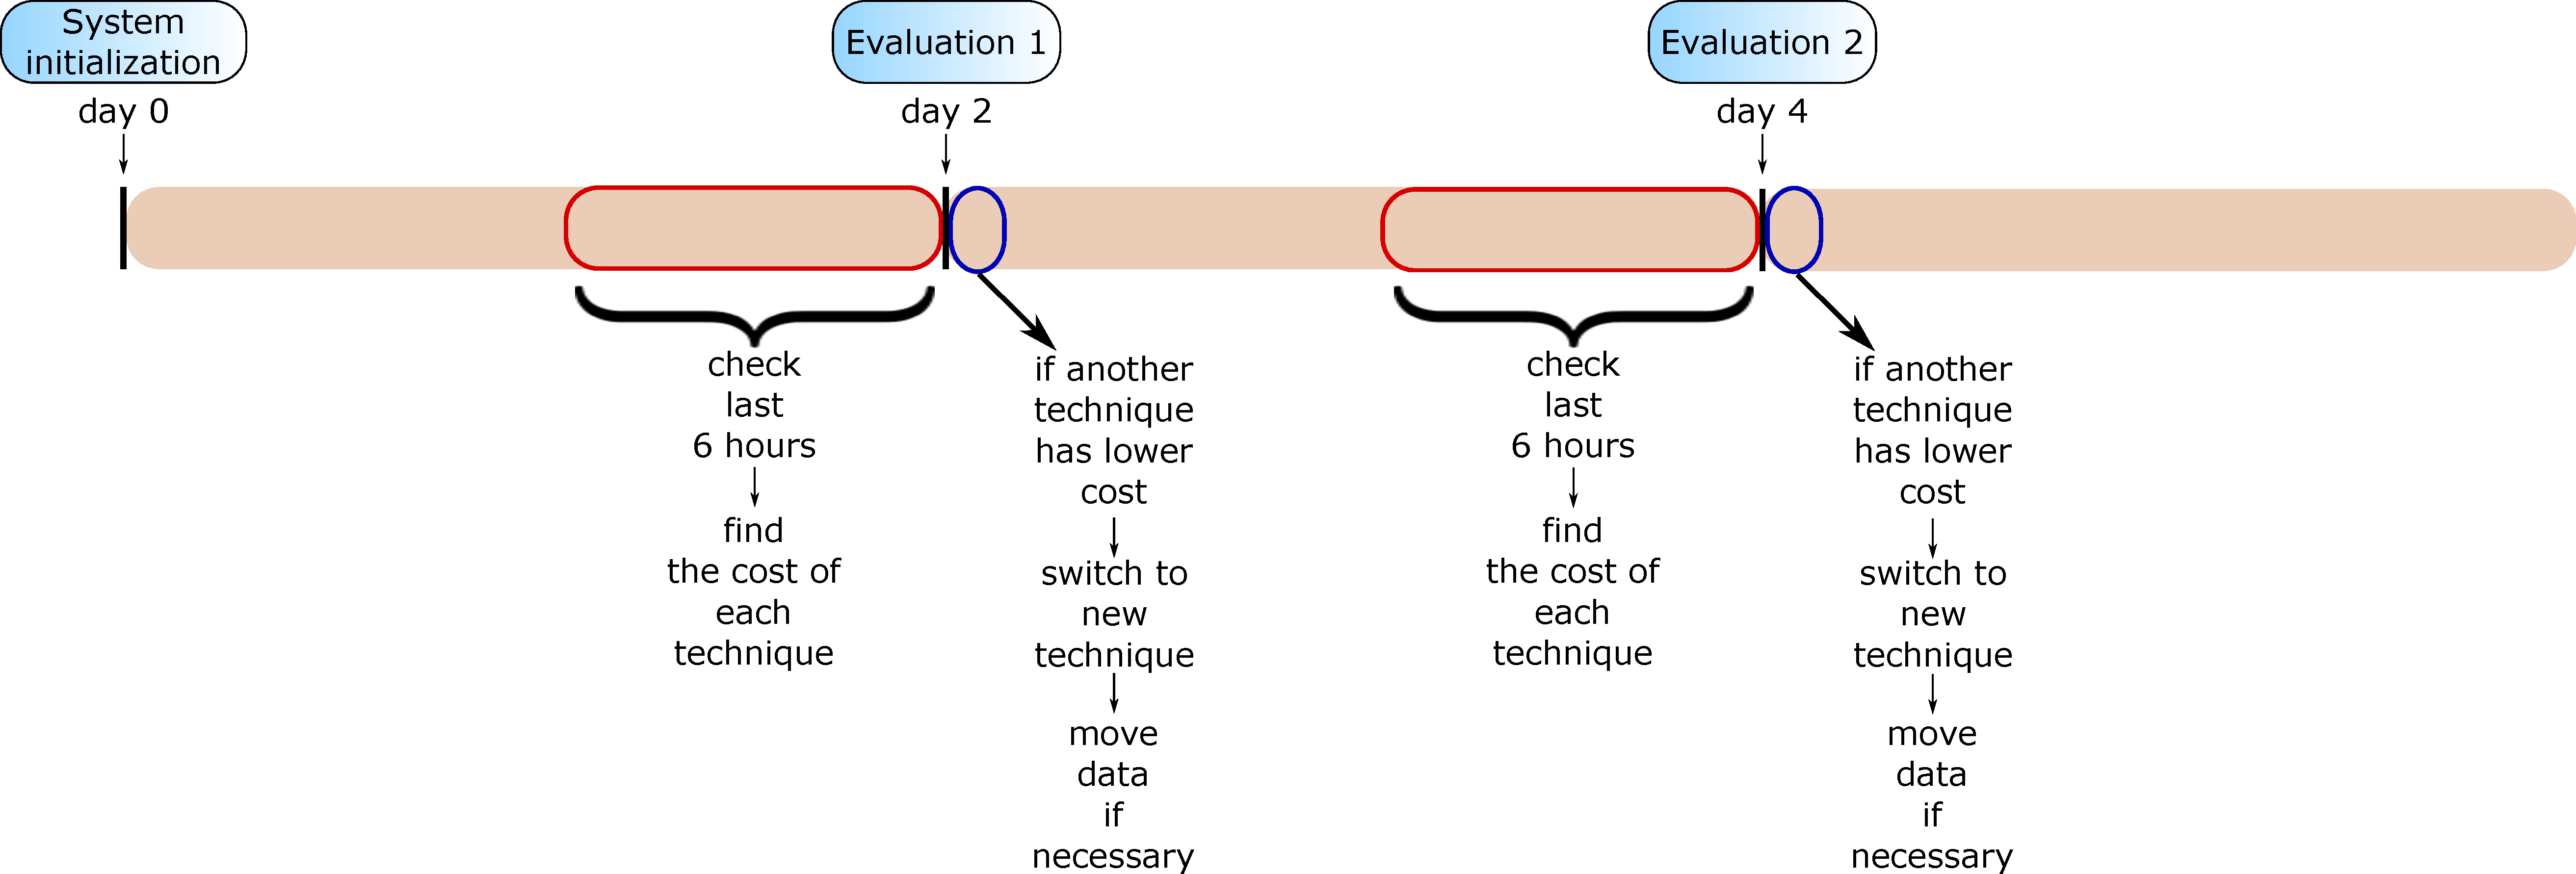
\includegraphics[width=\columnwidth,keepaspectratio]{FIG3.pdf}
\caption{Example of the Dynamic Greedy scheme (evaluations done at every 2 days, last 6 hours are checked only)}
\label{greedy_examples}
\end{figure}

\subsection{Correlation-Based Scheme}
\label{correlation}
This scheme is similar to the \textit{Dynamic Greedy Scheme} described in Section~\ref{greedy}, in the sense that
the node allocations are evaluated periodically at \textit{evaluation points} over a recent period (called
as \textit{control period}). However, rather than switching between node allocation
techniques (balancing, sequential, random, grouping) at \textit{evaluation points}, \textit{Correlation-Based Scheme}
starts with one of these techniques (can be chosen randomly) and keeps using that technique unless it is manually
changed. \textit{Correlation-Based Scheme} monitors user activities over the recent \textit{control period} and
allocates the same subset of cloud storage nodes to the users who tend to use the system in similar fashion.
Here, we define the similarity between users as concurrent usage of the cloud storage system, meaning that if
two or more users use the cloud storage system for longer than a threshold (called as \textit{similarity threshold}
in Algorithm~\ref{corrapp}) cumulatively, then same subset of storage nodes are allocated for them. We need
user access times as the metadata information to find concurrent user accesses, but other metadata (i.e.
number of accesses, amount of data stored) can be used as well to assess similarity between users.
Figure~\ref{correlation_examples} gives a numerical example of the \textit{Correlation-Based Scheme}.

\begin{figure}[!htbp]
\centering
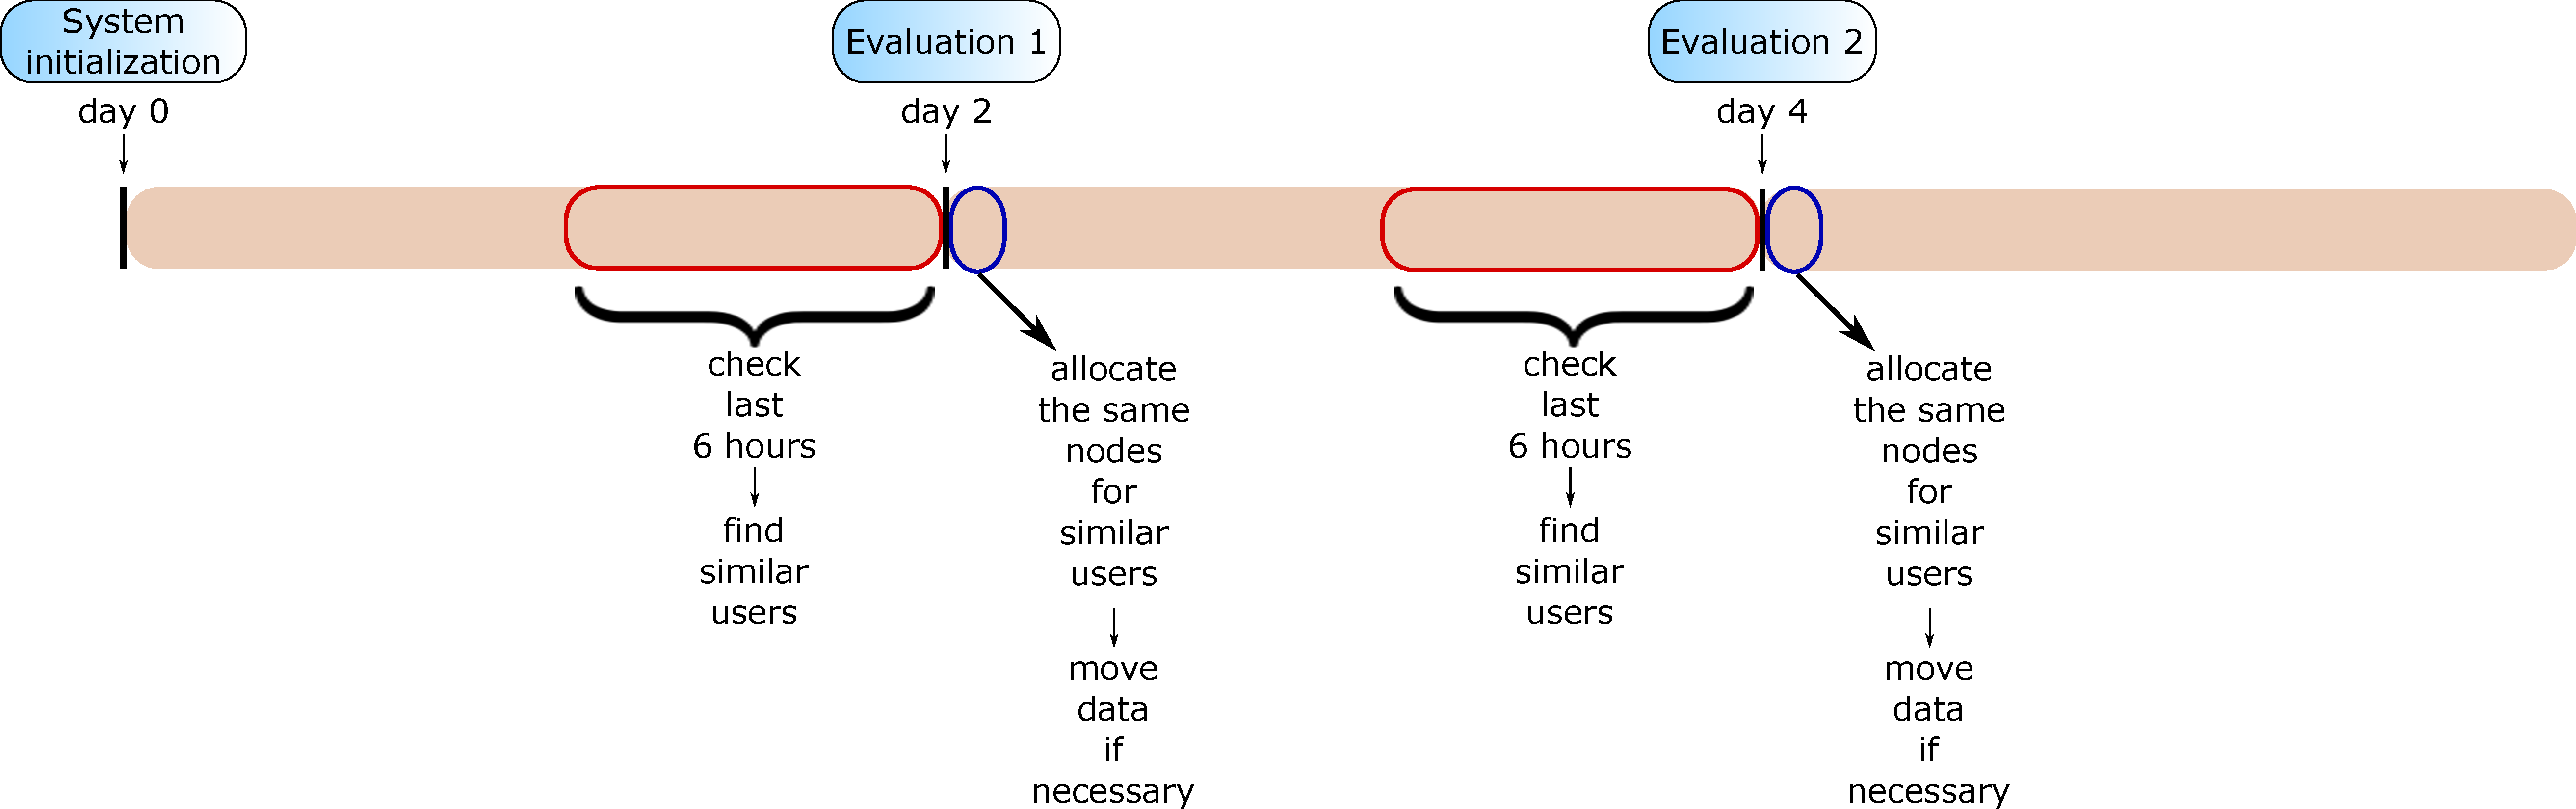
\includegraphics[width=\columnwidth,keepaspectratio]{FIG4.pdf}
\caption{Example of the Correlation-Based scheme (evaluations done at every 2 days, last 6 hours are checked only)}
\label{correlation_examples}
\end{figure}

The \textit{similarity threshold} sets a lower limit to define the concurrent usage of the storage system. As
an example, if the \textit{similarity threshold} is 4 hours, two or more users using the cloud storage systems
for more than 4 hours cumulatively are going to be assigned the same storage nodes. Here, it is important to point
out that the \textit{Correlation-Based Scheme} evaluates concurrent user activities cumulatively, meaning that, if
two or more users access the system concurrently for 3 hours in the morning and then for 1 hour in the afternoon,
those users will be considered as using the storage system in a similar fashion and they will be assigned the
same subset of cloud storage nodes. The \textit{Correlation-Based Scheme} is described in
Algorithm~\ref{corrapp}. 

\begin{algorithm}[!htbp]
\caption{Correlation-Based Scheme}
\label{corrapp}
\begin{algorithmic}[1]
    \STATE $T_{similar} \Leftarrow Similarity\ threshold$
    \STATE $R \Leftarrow Number\ of\ similarities\ between\ users\ in\ the\ most\ recent\ control\ period$
    \STATE $Similarities[\ ] \Leftarrow Array\ storing\ duration\ of\ user\ similarities$
    \FOR{$i=1$ to $R$}
        \IF{$Similarities[i] > T_{similar}$}
            \STATE Allocate the same storage nodes for users in this similarity
        \ENDIF
    \ENDFOR
\end{algorithmic}
\end{algorithm}


In order to tackle the energy efficiency problem of cloud storage systems, we propose
allocating nodes for each user based on the metadata information of that user
and switch the inactive nodes to low energy modes. As described earlier, we assume
a use scenario where a subset of the storage nodes max out the
available bandwidth of the system due to incasting. Therefore, it is not feasible to allocate more
than $M$ nodes to each user both for performance and energy efficiency reasons. Here $M$
represents the number of storage nodes in a subset allocated for a user. Therefore,
the problem we are trying to solve is how to map subsets of the storage nodes to the users.
Since user metadata heterogeneity is well-defined in large-scale cloud systems, we
retrieve user metadata information (i.e. user id, usage pattern) and
allocate subsets of storage nodes to the users using this information.

In this work, we propose three different methods to map cloud storage nodes to the
cloud users, summarized as follows:

\begin{itemize}
\item \textit{Fixed Scheme}: There
are four node allocation techniques in this method: \textit{balancing}, \textit{sequential},
\textit{random} and \textit{grouping} and once one of these techniques is chosen for a
cloud storage system, it remains in effect unless manually changed.
\item \textit{Dynamic Greedy Scheme}: This method
extends the \textit{Fixed Scheme} method by periodically doing dynamic reallocation
among one of the four
allocation techniques (\textit{balancing, sequential, random, grouping}) depending
on their costs. The cost of each technique is calculated based on how important it is
for the cloud storage system to save energy or to balance load.
\item \textit{Correlation-Based Scheme}: This method
monitors user activities and tries to allocate the same subset of storage nodes to the
users who tend to use the cloud storage system concurrently.
\end{itemize}

The energy-aware node allocation methods proposed here are designed to work for a traditional
distributed storage system architecture, but they could also work in a disk array. The
proposed methods not only reduce energy consumption, but also balance load on storage
nodes depending on metrics selected by the cloud administrators.

Before describing each node allocation method in more detail, we first list some of the usage
assumptions in our system and then explain two common
features of the node allocation methods: \textit{inactivity threshold} and \textit{job overlapping}.

We assume that;
\begin{itemize}
\item All storage nodes are initially off and a storage node is started up as soon as a
job arrives.
\item A user uses the same amount of storage space on each of its allocated nodes.
\item Any job run by a user is divided into equal tasks on the nodes allocated for
that user and these tasks are executed concurrently, meaning that they start and
complete simultaneously.
\item If a user is transferred from a subset of the storage nodes to another subset of
the storage nodes, this includes transferring only data. Any jobs that were executed
in the old subset of the storage nodes still belong to those nodes.
\end{itemize}

\paragraph{Inactivity Threshold}
The node allocation methods we are proposing try to save as much energy as possible and
also balance the load on storage nodes depending on metrics selected by the cloud administrators.
If a storage node is not allocated for any user at all, then it will stay in a low-energy mode.
On the other hand, if a storage node is allocated for one or more users, that node will
only switch to a low-energy mode after all jobs using that node are completed.
In an HPC system, the completion time of jobs can be predicted because of job scheduling systems.
Thus, we can decide when to switch a node to a low-energy mode. However, in a cloud storage system,
this predictability is not necessarily always possible, and we need to have a condition to decide when to switch a 
storage node to a low-energy mode. We call this metric the \textit{inactivity threshold}, which
can be defined as \textit{the period of time a node continues to operate at full capacity after the
completion of the most recent storage system job}. This means that, once a node stays inactive for
longer than the inactivity threshold, it can be switched to a
low-energy mode. The \textit{inactivity
threshold}, in this sense, is similar to \textit{break-even time} in previous studies, which ensures
that the energy saved by turning off a node is greater than the energy consumed while switching
that node from active to low-power modes.

In our work, we define the low-energy mode as the state where a node is completely turned off. However,
some modern hard drives have the ability to operate at various
speeds~\cite{Gurumurthi:2003:DDS:871656.859638} thus providing
different levels of energy utilization.
Therefore, in order to conserve energy it is not mandatory to completely turn off a node. Depending on how
much energy saving is demanded by the user, the node allocation techniques can switch nodes into
low-speed operating modes without turning them off. In this work, in order to show the effect of the
node allocation methods better, we assume the worst case and turn off a storage node in low-energy
mode.

If a user is allocated to a node that has been turned off, then that
node needs to start operating at full capacity again. In this case, the user can not immediately access
that storage node, since it will take some time for that node to run at full capacity again. We define the time
it takes to start up a completely turned-off node as the \textit{startup time}. If a storage node has been inactive
between two jobs for longer than the \textit{inactivity threshold}, then the next job on that node
will have to wait for the node to start up.

The \textit{inactivity threshold} and the \textit{startup time} are
important parameters in determining how a real cloud storage
system is going to be affected by the node assignment methods we are proposing.

\paragraph{Job Overlapping}
In a large-scale cloud storage system, each storage node may be used by multiple concurrent users. Our node allocation
methods might allocate a node to multiple users. Therefore, concurrent users can simultaneously
run jobs that use a particular storage node. When two or more jobs overlap on a node, we assume that
node still consumes the same energy per unit
time~\cite{Tsirogiannis:2010:AEE:1807167.1807194}. In other words,
we assume the increased activity due to the multiple jobs will not
increase energy consumption significantly. This is, for the most
part, true because most of the energy is consumed by spinning the
drives not by moving actuators on the drive.

\subsection{Fixed Scheme}
\label{fixed}
In this first scheme, one of the four node allocation techniques described below 
(balancing, sequential, random or grouping) is chosen by the cloud
storage system administrator
and is kept fixed unless manually changed. All techniques have one goal
in common - exploiting user metadata to allocate storage nodes for users. Individually,
each technique performs differently in terms of uniformly allocating storage nodes.
These techniques are each described numerically in Figure~\ref{fixed_examples} with examples.

\begin{figure}[!htbp]
\centering
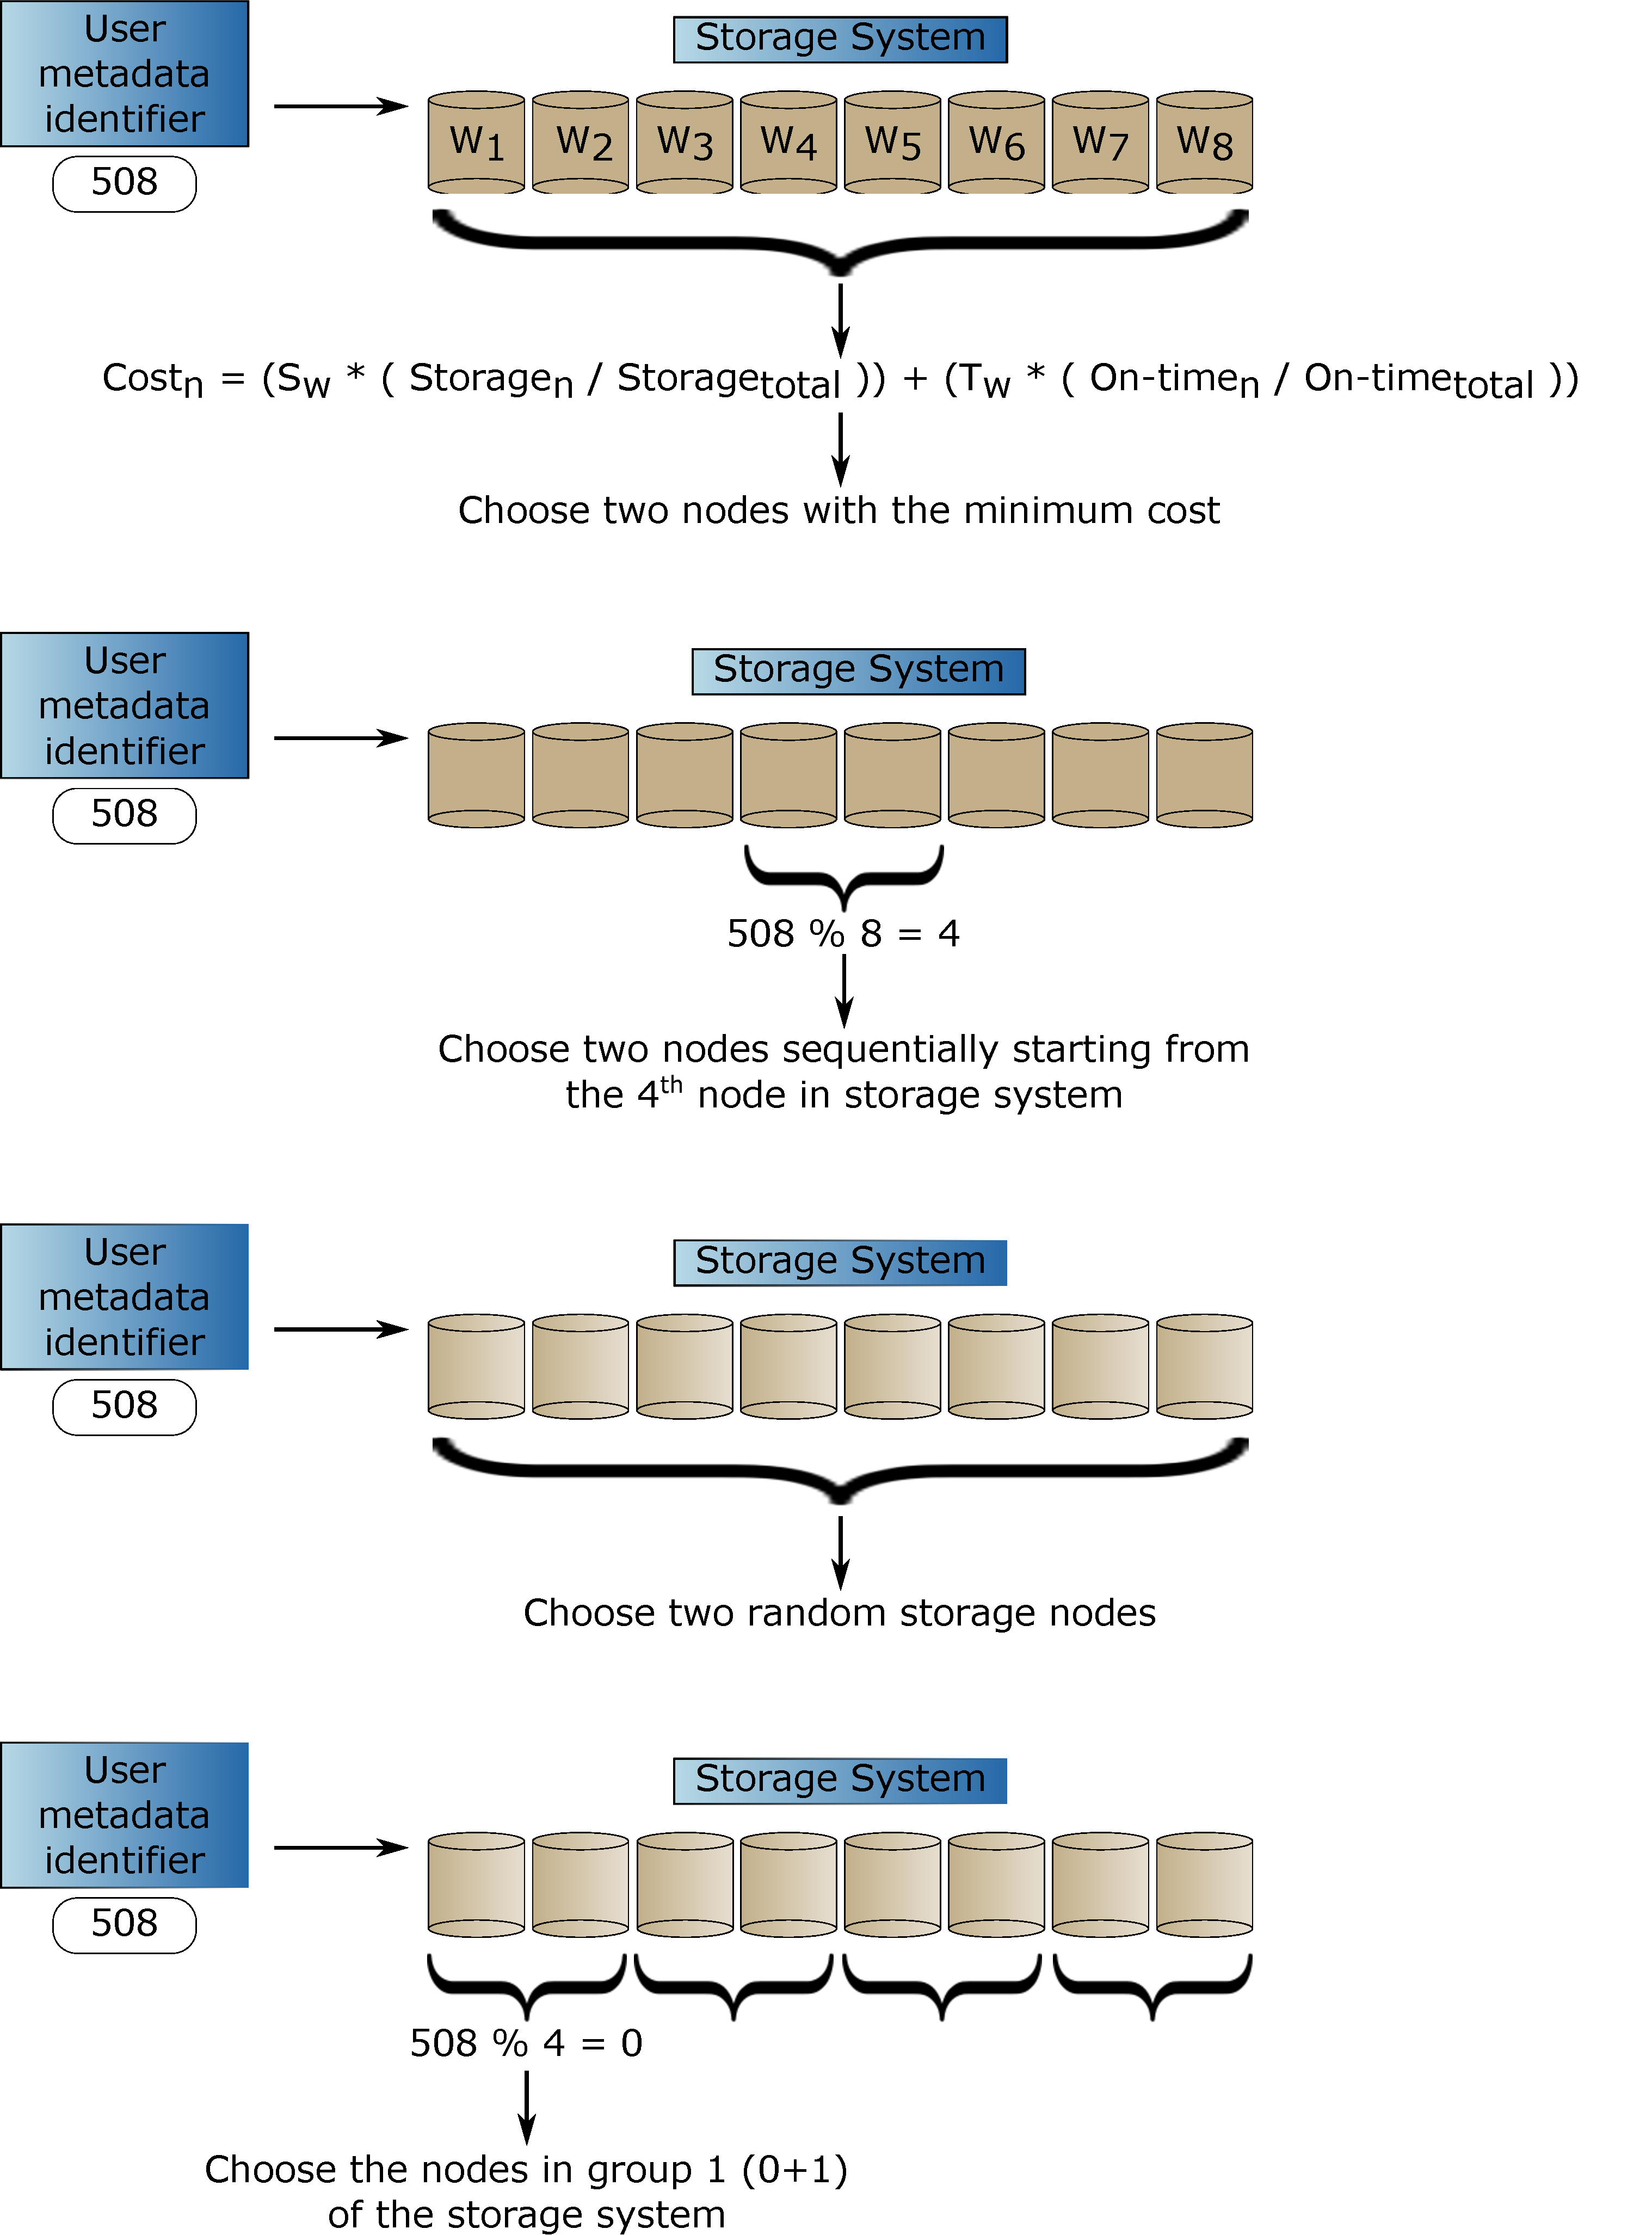
\includegraphics[width=\columnwidth,keepaspectratio]{FIG2.pdf}
\caption{Examples of the node allocation techniques in the Fixed scheme}
\label{fixed_examples}
\end{figure}

\subsubsection{Balancing Technique}
\label{baltechnique}
The primary goal of this technique is to balance the load across the cloud storage nodes. We
define the \textit{load} here in two different ways:

\begin{itemize}
\item The amount of data stored on each node.
\item The total time each node stays on serving user requests.
\end{itemize}

We call balancing the amount of data stored on each node \textit{storage space balancing}.
Similarly, balancing the total time each node stays on is
called \textit{on-time balancing}. These two balancing
techniques ensure that all the nodes in the system are used equally.
Otherwise, the simplest energy saving technique is to simply put all
users and data on the same subset of nodes and permanently turn off
all other nodes. This, however, can cause capacity issues as the
selected nodes may not have enough storage space and also incurs
higher utilization and thus, higher failure rates.
The balancing technique enables system administrators to specify weights for \textit{storage space
balancing} and \textit{on-time balancing} to indicate their importance and allocates
storage nodes for users by adhering to these weights. A \textit{cost} metric is calculated for every
storage node in the system by multiplying storage space and on-time weights with the normalized 
storage space and on-time on that node respectively. In order to normalize storage space and
on-time values, they are divided by the total amount of storage and on-time on all nodes
respectively. In the end, storage nodes with lower costs are preferred by the balancing technique
with the eventual goal of uniformly distributing storage space usage and on-time across storage nodes.
As mentioned previously, we assume the storage space usage of a user is distributed evenly across the
nodes allocated for that user and a job running on multiple nodes concurrently takes the same amount
of time to complete on each node.

Assuming, $N$ is the total number of nodes in the cloud storage system and $M$ is the number
of storage nodes allocated for each user, the balancing technique works as shown in Algorithm~\ref{balapp}.

\begin{algorithm}[!htbp]
\caption{Balancing Technique}
\label{balapp}
\begin{algorithmic}[1]
    \STATE $N \Leftarrow$ Total\ number\ of\ storage\ nodes
    \STATE $M \Leftarrow$ Number\ of\ storage\ nodes\ to\ allocate\ for\ the\ user
    \STATE $ChosenNodes[\ ] \Leftarrow$ Nodes\ that\ will\ be\ allocated\ for\ the\ user
    \STATE $S_{total} \Leftarrow$ Total\ amount\ of\ data\ stored\ on\ all\ nodes
    \STATE $T_{total} \Leftarrow$ Total\ duration\ of\ time\ all\ nodes\ stayed\ on
    \STATE $S_i \Leftarrow$ Amount\ of\ data\ stored\ on\ node\ $i$
    \STATE $T_i \Leftarrow$ Duration\ of\ time\ node\ $i$ stayed\ on
    \STATE $S_W \Leftarrow$ Importance\ of\ balancing\ storage\ space
    \STATE $T_W \Leftarrow$ Importance\ of\ balancing\ time
    \STATE $Costs[\ ] \Leftarrow$ Costs\ of\ nodes\ $i$
    \FOR{$i=1$ to $N$}
        \STATE $Costs[i] \Leftarrow (S_W * (S_i/S_{total}) + (T_W * (T_i/T_{total}))$
    \ENDFOR
    \FOR{$i=1$ to $M$}
        \STATE $ChosenNodes[i] \Leftarrow min(Costs[\ ])$
        \STATE Remove $min(Costs[\ ])$ from $Costs[\ ]$
    \ENDFOR
\end{algorithmic}
\end{algorithm}

The storage space and on-time weights should add up to 1. As an example, if it is equally important
to balance storage space and on-time for a system
administrator, then $S_W=T_W=0.5$. However, if it is more important to
balance storage space, then $S_W=1$ and $T_W=0$.

\subsubsection{Sequential Technique}
\label{seqtechnique}
The sequential technique use an approach similar to consistent hashing~\cite{Karger:1997:CHR:258533.258660}.
%Assuming $N$ is the total number of nodes in the cloud storage system and $M$ is the number
%of storage nodes allocated for each user;
The approach starts by calculating an $Offset$
value for a given user
with metadata information represented by $I$. As described earlier, 
this metadata information can be a user id or user home directory, basically any metadata information
that can be hashed to an integer.

Given this hash value, one can then sequentially allocate storage nodes for the user starting from
the storage node with an identifier equal to $Offset$.
%Considering that nodes in distributed storage
%systems are usually given numbers such as \textit{(001,002,...)} to indicate their order, this is a
%reasonable approach. As we mentioned earlier, $M$ is the number of storage nodes allocated for
%each user.
The $M$ nodes following the storage node with identifier equal to $Offset$ are
allocated for a user in the sequential technique.
%Assuming, $N$ is the total number of nodes in the
%cloud storage system and $M$ is the number of storage nodes allocated
%for each user
A summary of the sequential
technique is shown in Algorithm~\ref{seqapp}.

\begin{algorithm}[!htbp]
\caption{Sequential Technique}
\label{seqapp}
\begin{algorithmic}[1]
    \STATE $N \Leftarrow$ Total\ number\ of\ storage\ nodes
    \STATE $M \Leftarrow$ Number\ of\ storage\ nodes\ to\ allocate\ for\ the\ user
    \STATE $I \Leftarrow$ Metadata\ information\ of\ the\ user
    \STATE $Offset \Leftarrow$ Identifier\ of\ storage\ node\ from\ which\ allocation\ will\ start
    \STATE $ChosenNodes[\ ] \Leftarrow$ Nodes\ that\ will\ be\ allocated\ for\ the\ user
    \STATE $Offset \Leftarrow I\ mod\ N$
    \FOR{$i=1$ to $M$}
        \STATE $ChosenNodes[i] \Leftarrow (Offset\ +\ i)\ mod\ M$
    \ENDFOR
\end{algorithmic}
\end{algorithm}

Note that in Algorithm~\ref{seqapp} on line 6, we are taking the modulus of node identifiers in order to
make sure they are smaller than the total number of nodes in the cloud
storage system, $N$.
%This is because the starting offset calculated in the the sequential technique may be close to the last
%storage node in the system, such that when $M$ storage nodes are sequentially assigned to a user,
%we may run out of storage nodes in the system. In this case the node allocation continues with the
%first storage node.

\subsubsection{Random Technique}
The random technique uses a random number generator that chooses an identifier of a storage node
in the system. The random number generator is called $M$ times to generate $M$ different identifiers.
These identifiers represent the storage nodes that will be allocated for a user. The
random function is seeded with the user's arrival time to the storage system, giving enough
randomness. Still, if it produces an identifier twice, it is called until all $M$ identifiers
in the subset are distinct. Assuming, $N$ is the total number of nodes in the
cloud storage system and $M$ is the number of storage nodes allocated for each user, the random
technique works as shown in Algorithm~\ref{randapp}.

\begin{algorithm}[!htbp]
\caption{Random Technique}
\label{randapp}
\begin{algorithmic}[1]
    \STATE $N \Leftarrow Total\ number\ of\ storage\ nodes$
    \STATE $M \Leftarrow Number\ of\ storage\ nodes\ to\ allocate\ for\ the\ user$
    \STATE $ChosenNodes[\ ] \Leftarrow Nodes\ that\ will\ be\ allocated\ for\ the\ user$
    \FOR{$i=1$ to $M$}
        \WHILE{$j\ \in ChosenNodes[\ ]$}
            \STATE $j \Leftarrow rand()$
        \ENDWHILE
        \STATE $ChosenNodes[i] \Leftarrow j$
    \ENDFOR
\end{algorithmic}
\end{algorithm}

\subsubsection{Grouping Technique}
The grouping technique is similar to the sequential technique described in Section~\ref{seqtechnique}.
Compared to the sequential technique, the grouping technique has fewer starting points(\textit{offset})
to choose. %Assuming, $N$ is the total number of nodes in the cloud storage system and $M$ is the
%number of storage nodes allocated for each user;
First, node groups of size $M$ are
created where $M$ sequential storage nodes together form a
group. Here, for ease of explanation, we 
assume that total number of nodes, $N$, is a multiple of the number of storage nodes allocated
for each user, $M$. For systems where this is not true, groups may be overlapped. At this point,
we assume $G\ =\ N\ /\ M$ groups are created in the systems, where $G$ denotes the number of groups created. 
Then, similar to the sequential technique, a group is chosen using the given user's metadata information
represented by $I$ and the storage nodes in that group are allocated for that user. As described
earlier, this metadata information can be user id or user home directory, basically any metadata
information that can be hashed to an integer. The grouping technique works as shown in
Algorithm~\ref{groupapp}.

\begin{algorithm}[!htbp]
\caption{Grouping Technique}
\label{groupapp}
\begin{algorithmic}[1]
    \STATE $N \Leftarrow$ Total\ number\ of\ storage\ nodes
    \STATE $M \Leftarrow$ Number\ of\ storage\ nodes\ to\ allocate\ for\ the\ user
    \STATE $G \Leftarrow$ Number\ of\ storage\ node\ groups
    \STATE $I \Leftarrow$ Metadata\ information\ of\ the\ user $\Leftarrow N\ /\ M$
    \STATE $Offset \Leftarrow$ Identifier\ of\ node\ group\ which\ will\ be\ allocated\ for\ the\ user
    \STATE $ChosenNodes[\ ] \Leftarrow$ Nodes\ that\ will\ be\ allocated\ for\ the\ user
    \STATE $Offset \Leftarrow I\ mod\ G$
    \FOR{$i=1$ to $M$}
        \STATE $ChosenNodes[i] \Leftarrow (G\ *\ M)\ +\ i$
    \ENDFOR
\end{algorithmic}
\end{algorithm}

\subsection{Dynamic Greedy Scheme}
\label{greedy}
In this method, one of the four node allocation techniques described in Section~\ref{fixed} (balancing,
sequential, random or grouping) is initially chosen by the cloud system and that technique is re-evaluated
against other techniques at certain times (called as \textit{evaluation points}) over a recent period (called
as \textit{control period}), in terms of energy efficiency and/or load balancing. If there is a better
technique in terms of energy efficiency and/or load balancing and if the cost of switching to that technique
is less than the energy to be saved by switching to that technique, then the current technique is changed.
The \textit{Dynamic Greedy Scheme} is described in Algorithm~\ref{greedyapp}.

In this scheme, we use coefficient or variation (CV) amongst the nodes as a proxy for storage space
and on-time balancing.
In other words, a high CV indicates that the storage
space or on-time is not well balanced.
The \textit{Dynamic Greedy Scheme} first multiplies the normalized CVs of storage space
and on-time ($Svar$ and $Tvar$ in Algorithm~\ref{greedyapp}) with their corresponding importance
weights ($S_W$ and $T_W$). In order to normalize the CVs of storage space and on-time, they are
divided by the maximum possible CV of storage space ($MaxSvar$) and on-time
($MaxTvar$) respectively. The maximum CV of storage space and on-time occurs when all requests
are served by a single storage node and this sets an upper limit on the CV value. Then the multiplication
of the normalized energy cost ($ECost$) with the energy consumption weight ($E_W$) is added to this product. Energy
cost includes both the energy consumption due to running jobs according to a technique ($JobCost$) and the energy
consumption due to transferring user data while switching to that technique ($TrnCost$). Energy cost ($ECost$) is
divided by the sum of maximum cost of jobs ($MaxJobCost$) and the maximum cost of data transfers ($MaxTrnCost$) over the 
\textit{control period}. Maximum job cost ($MaxJobCost$) occurs when all nodes are left on all the time. Maximum data
transfer cost ($MaxTrnCost$) occurs when all data existing in the storage system is moved.

A cloud system administrator can specify different values for storage space, on-time and energy consumption
weights ($S_W$, $T_W$ and $E_W$). This enables a fine-grained control over load-balancing and energy consumption
in a cloud storage system. As discussed in Section~\ref{baltechnique}, the storage space
and on-time weights add up to 1. The energy consumption weight is independent of the other two, meaning that,
a cloud system administrator might prefer to save energy regardless of load-balancing decisions. 

\begin{algorithm}[!htbp]
\caption{Dynamic Greedy Scheme}
\label{greedyapp}
\begin{algorithmic}[1]
    \STATE $P \Leftarrow$ Number\ of\ available\ node\ allocation\ techniques
    \STATE $S_W \Leftarrow$ Importance\ of\ balancing\ storage\ space
    \STATE $T_W \Leftarrow$ Importance\ of\ balancing\ time
    \STATE $E_W \Leftarrow$ Importance\ of\ reducing\ energy\ consumption
    \STATE $Svar_i \Leftarrow$ CV\ of\ storage\ space\ across\ all\ nodes\ for\ technique\ $i$
    \STATE $MaxSvar \Leftarrow$ Maximum\ possible\ CV\ of\ storage\ space\ across\ all\ nodes
    \STATE $Tvar_i \Leftarrow$ CV\ of\ on-time\ across\ all\ nodes\ for\ technique\ $i$
    \STATE $MaxTvar \Leftarrow$ Maximum\ possible\ CV\ of\ on-time\ across\ all\ nodes
    \STATE $JobCost_i \Leftarrow$ Cost\ of\ all\ jobs\ in\ the\ control\ period\ for\ technique\ $i$
    \STATE $TrnCost_i \Leftarrow$ Cost\ of\ data\ transfers\ while\ switching\ to\ technique\ $i$
    \STATE $ECost_i \Leftarrow JobCost_i + TrnCost_i$
    \STATE $MaxJobCost \Leftarrow$ Maximum\ cost\ of\ all\ jobs\ \ over\ the\ control\ period
    \STATE $MaxTrnCost \Leftarrow$ Maximum\ cost\ of\ all\ data\ transfers\ over\ the\ control\ period
    \STATE $TotalCost_i \Leftarrow$ Total\ cost\ of\ technique\ i\ at\ an\ evaluation\ point
    \STATE $MinCost \Leftarrow$ Minimum\ technique\ cost\ observed\ so\ far
    \STATE $NewTechq \Leftarrow$ Technique\ that\ will\ be\ in\ affect\ after\ the\ evaluation

    \STATE $MinCost \Leftarrow 0$
    \STATE $NewTechq \Leftarrow 0$
    \FOR{$i=1$ to $P$}
        \STATE $TotalCost_i \Leftarrow (S_W\ *\ (Svar_i\ /\ MaxSvar))\ +\ (T_W\ *\ (Tvar_i\ /\ MaxTvar))\ +\ (E_W\ *\ (ECost_i\ /\ (MaxJobCost\ +\ MaxTrnCost)))$
        \IF{$MinCost == 0\ \OR\ TotalCost_i < MinCost$}
            \STATE $NewTechq \Leftarrow i$
            \STATE $MinCost \Leftarrow TotalCost_i$
        \ENDIF
    \ENDFOR
\end{algorithmic}
\end{algorithm}

The parameters of a technique evaluation can be summarized as follows:
\begin{itemize}
\item \textbf{The frequency of the technique evaluations}: The system administrator might decide to
evaluate the current node allocation technique of the system against other techniques every couple of
hours, days etc.
\item \textbf{Jobs to evaluate}: Ideally, all jobs that have been submitted to the storage system so far
should be evaluated to compare node allocation techniques with each other. However, this might prove to be costly due
to the potentially large number of jobs submitted before an \textit{evaluation point}. Therefore, the system
administrator specifies a \textit{control period} that specifies the
time period from which the jobs are used to evaluate the node
allocation techniques at every \textit{evaluation point}.
The \textit{control period} again can be couple of hours, days etc., but it has to be less than the frequency of
technique evaluations to make sure that evaluations at different moments do not interfere with each other.
\item \textbf{What is important while comparing node allocation techniques}: Cloud system administrators might be
concerned with different aspects of the cloud storage system. As an example, different values can be specified for
storage space, on-time and energy consumption weights ($S_W$, $T_W$ and $E_W$)
\end{itemize}

Figure~\ref{greedy_examples} gives a numerical example of
the \textit{Dynamic Greedy Scheme}.
A cloud storage system administrator can evaluate node allocation techniques (balancing, sequential, random,
grouping) every 4 days by looking at the jobs submitted in the last 6 hours and by trying to save as much energy
as possible while trying to balance the storage space only across the nodes. Our work in this sense is similar
to the studies that try to predict idle periods or node reservation lengths~\cite{4724317, Riska:2010:FRE:1710115.1710124},
but the way we are predicting the future is much simpler compared to those studies. We simply look at the jobs
going back to a specified duration of time (a.k.a. \textit{control period}). However, existing studies instrument
and monitor cloud systems with complex mechanisms to collect feedback and hints.

\begin{figure}[!htbp]
\centering
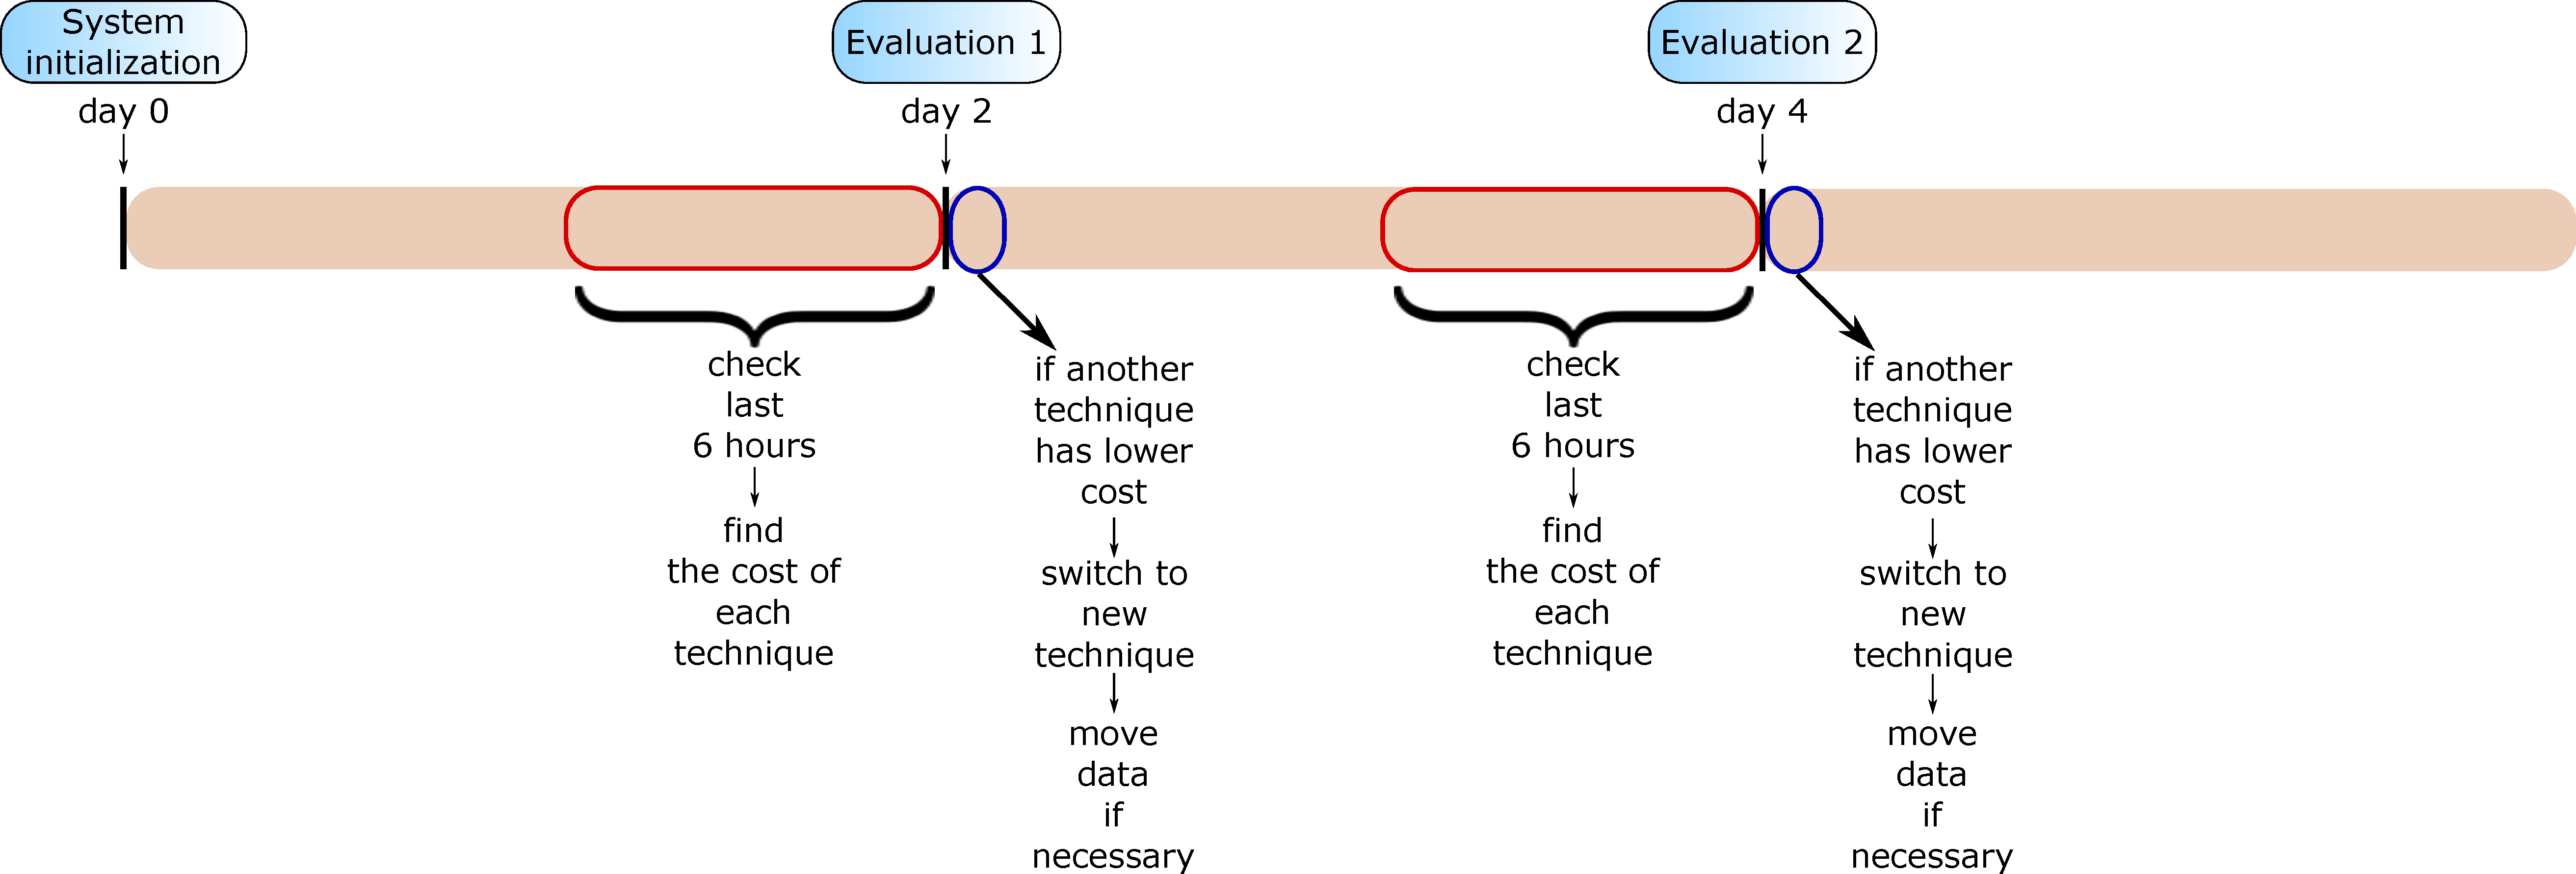
\includegraphics[width=\columnwidth,keepaspectratio]{FIG3.pdf}
\caption{Example of the Dynamic Greedy scheme (evaluations done at every 2 days, last 6 hours are checked only)}
\label{greedy_examples}
\end{figure}

\subsection{Correlation-Based Scheme}
\label{correlation}
This scheme is similar to the \textit{Dynamic Greedy Scheme} described in Section~\ref{greedy}, in the sense that
the node allocations are evaluated periodically at \textit{evaluation points} over a recent period (called
as \textit{control period}). However, rather than switching between node allocation
techniques (balancing, sequential, random, grouping) at \textit{evaluation points}, \textit{Correlation-Based Scheme}
starts with one of these techniques (can be chosen randomly) and keeps using that technique unless it is manually
changed. \textit{Correlation-Based Scheme} monitors user activities over the recent \textit{control period} and
allocates the same subset of cloud storage nodes to the users who tend to use the system in similar fashion.
Here, we define the similarity between users as concurrent usage of the cloud storage system, meaning that if
two or more users use the cloud storage system for longer than a threshold (called as \textit{similarity threshold}
in Algorithm~\ref{corrapp}) cumulatively, then same subset of storage nodes are allocated for them. We need
user access times as the metadata information to find concurrent user accesses, but other metadata (i.e.
number of accesses, amount of data stored) can be used as well to assess similarity between users.
Figure~\ref{correlation_examples} gives a numerical example of the \textit{Correlation-Based Scheme}.

\begin{figure}[!htbp]
\centering
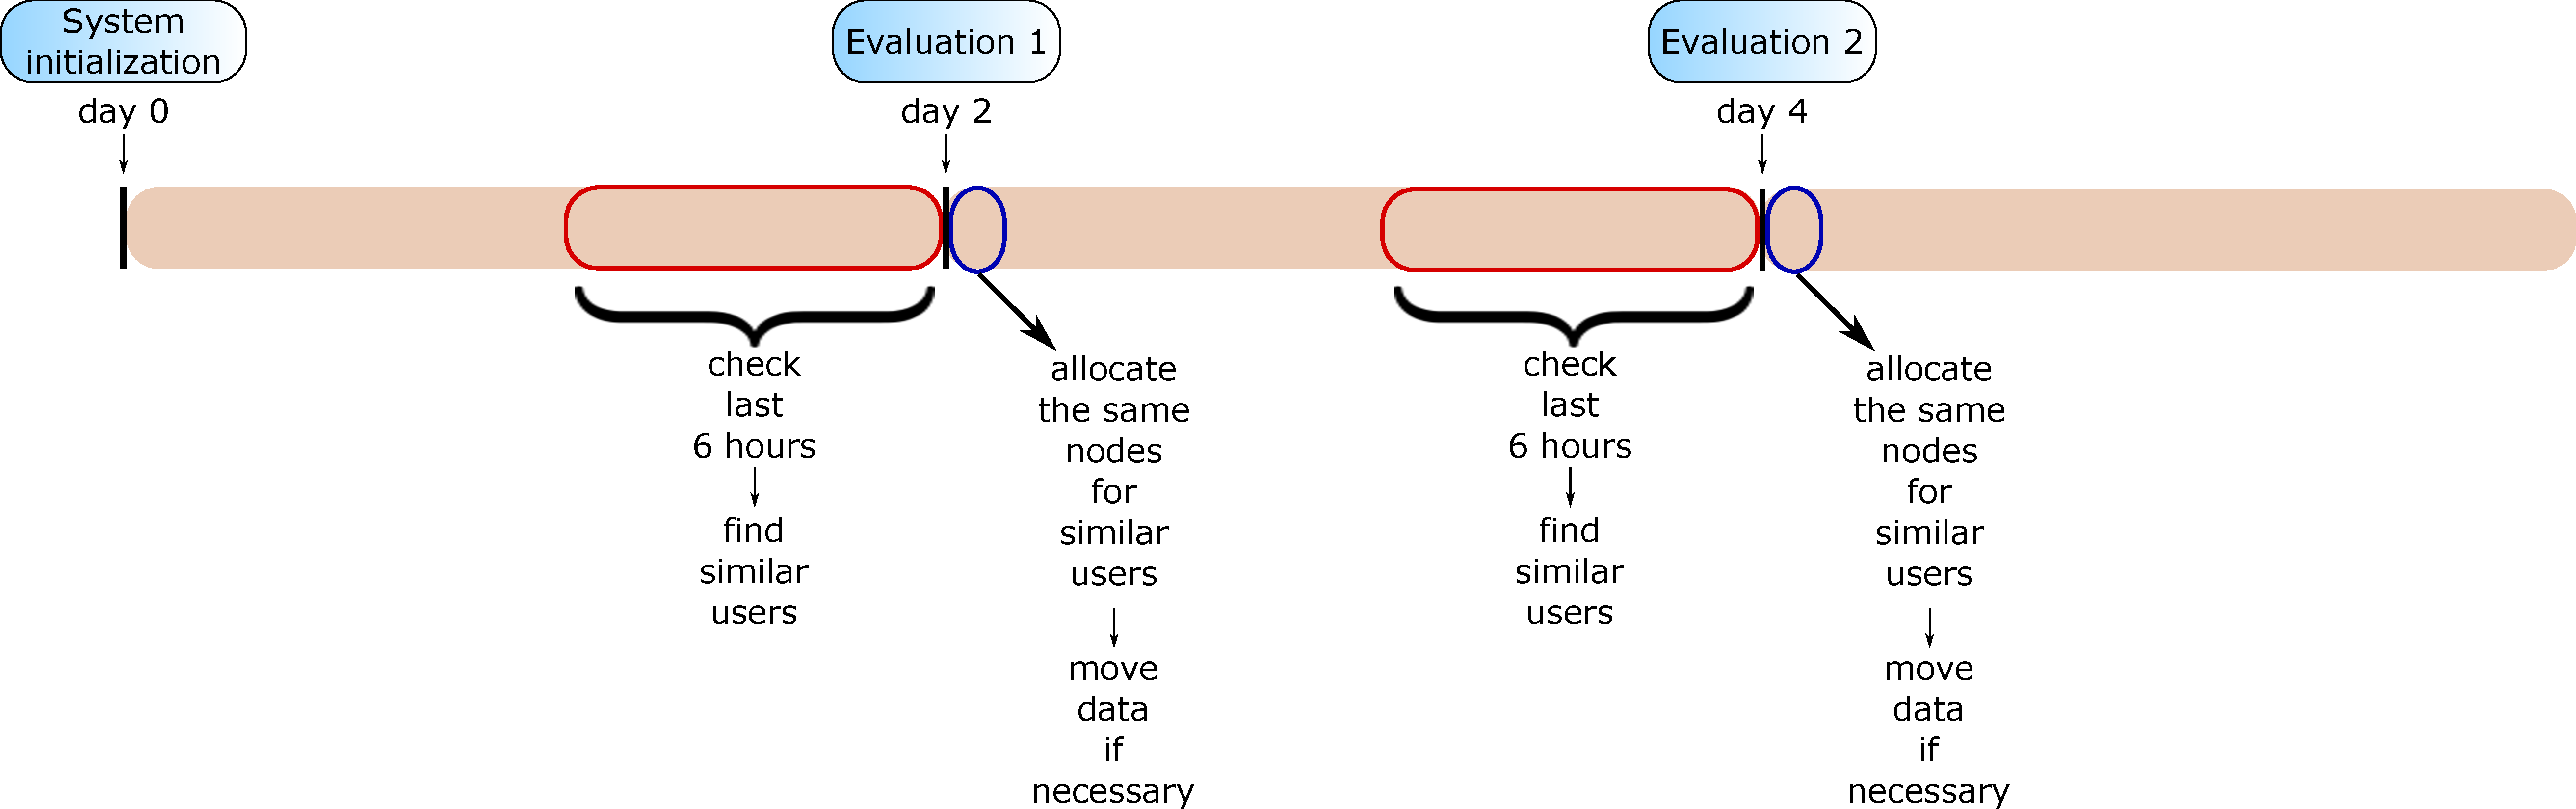
\includegraphics[width=\columnwidth,keepaspectratio]{FIG4.pdf}
\caption{Example of the Correlation-Based scheme (evaluations done at every 2 days, last 6 hours are checked only)}
\label{correlation_examples}
\end{figure}

The \textit{similarity threshold} sets a lower limit to define the concurrent usage of the storage system. As
an example, if the \textit{similarity threshold} is 4 hours, two or more users using the cloud storage systems
for more than 4 hours cumulatively are going to be assigned the same storage nodes. Here, it is important to point
out that the \textit{Correlation-Based Scheme} evaluates concurrent user activities cumulatively, meaning that, if
two or more users access the system concurrently for 3 hours in the morning and then for 1 hour in the afternoon,
those users will be considered as using the storage system in a similar fashion and they will be assigned the
same subset of cloud storage nodes. The \textit{Correlation-Based Scheme} is described in
Algorithm~\ref{corrapp}. 

\begin{algorithm}[!htbp]
\caption{Correlation-Based Scheme}
\label{corrapp}
\begin{algorithmic}[1]
    \STATE $T_{similar} \Leftarrow Similarity\ threshold$
    \STATE $R \Leftarrow Number\ of\ similarities\ between\ users\ in\ the\ most\ recent\ control\ period$
    \STATE $Similarities[\ ] \Leftarrow Array\ storing\ duration\ of\ user\ similarities$
    \FOR{$i=1$ to $R$}
        \IF{$Similarities[i] > T_{similar}$}
            \STATE Allocate the same storage nodes for users in this similarity
        \ENDIF
    \ENDFOR
\end{algorithmic}
\end{algorithm}


\section{Mathematical Model of the Problem}
\label{model}
%%In this section, we present a mathematical model to estimate the outcome
of the proposed methods with varying parameters. We are particularly interested
in estimating the energy consumption, latency per access and load balance as the outcomes
of the system. The methods we proposed distribute jobs in a workload across
all of the storage nodes, eventually creating time interval series on each
storage node. The main driving parameter of the mathematical model is these series of
time intervals. We consider three different time intervals;
\textit{interjobs, interarrivals} and \textit{job lengths}. Interjob is
the interval between the completion of a job and the start of the next
job. Interarrival is the interval between the start of a job and the
start of the next job. Job length is the interval between the start and
completion of a job. We collect these time series data for each workload
and storage node and fit them to probability distribution models in order
to estimate the energy consumption, latency per access and load balance.

In the proposed mathematical model, time series can be fitted to different
probability distribution models depending on the workload and the number
of jobs assigned to a storage node. As each workload can be fitted to
different probability distribution models on each storage node, we use
$F(t)$ to represent the cumulative distribution function (CDF) at this
point for ease of presentation. By definiton of the cumulative distribution function, $F_{X}(t)$ represents
the probability that the random variable $X$, i.e. the interarrival
time between jobs, is smaller than or equal to $t$.
$F(t)$ is replaced with the actual CDF
of each workload in Section~\ref{validate_model}.
%Similarly, $F(X+1) - F(X)$ represents the probability that the random variable
%$t$ is equal to $X$.

\subsection{Energy Consumption}
We first estimate the energy consumption of a storage node.
The average job length
on a storage node without taking any latencies into account can be
calculated by
looking at the jobs on a storage node and taking their average as shown in 
Equation~\eqref{eq_math_one}, where $N_{J}$ is the number of jobs on a
storage node, $J_{avg}$ is the average job length without latencies and $J(k)$
is the length of an individual job.

\begin{equation}
J_{avg} = \frac{\sum\limits_{k=1}^{N_{J}} J(k)}{N_{J}}
\label{eq_math_one}
\end{equation}  
\hfill

In order to estimate the impact of job latencies,
we consider four different cases for the interjob
times:

\begin{itemize}
\item The interjob time
is greater than the sum of the inactivity threshold ($T_I$) and the
startup time ($T_S$).
In this case, even if the job finishing before the interjob period experiences
latency, the interjob time will still be greater than the inactivity threshold and
therefore will cause the storage node to be turned off. In this case,
the next job
assigned to this storage node will experience latency equal to the startup
time, since it will have to wait for the storage node to be turned
on. The average latency impact is the probability that the interjob time
is larger than $(T_I+T_S)$ multiplied by $(T_I+T_S)$, or
$(1-F_{T_I+T_S}(t))*(T_I+T_S))$.

\item The interjob time
is greater than the inactivity threshold, but smaller than or equal to the sum of
the inactivity threshold and startup time. In this case, if the job finishing
before the interjob period experiences latency, the interjob time might become smaller
than the inactivity threshold. This will cause the storage node not to be turned
off at all and therefore to miss the opportunity to reduce energy consumption.
The average latency impact is the probability that the interjob time
is between $T_I$ and $T_I+T_S$ multiplied by
the interjob time, or $\int_{T_I}^{T_I+T_S}tF'(t)dt$.

\item The interjob time is
smaller than or equal to the inactivity threshold, but greater than the startup time. In this
case, even if the job finishing before the interjob period experiences latency,
the storage system will stay on until the next job arrives.
The average latency impact is the probability that the interjob time
is between $T_S$ and $T_I$ multiplied by
the interjob time, or $\int_{T_S}^{T_I}tF'(t)dt$.

\item The interjob time
is smaller than or equal to the startup time. In this case, if the job
finishing before the interjob period experiences latency, it might overlap
with the next job assigned to the storage node, as the latency it experiences
(startup time) will be greater than the interjob time. If there is an overlap
between jobs, that means we are reducing energy consumption.
The average latency impact is the probability that the interjob time
is less than $T_S$ multiplied by
the interjob time, or $-\int_{0}^{T_S}tF'(t)dt$.
\end{itemize}  

Putting these impacts together, we can estimate the average
job length with latencies as 
shown in Equation~\eqref{eq_math_two}.

\begin{equation}
\label{eq_math_two}
\begin{aligned}
J_{avg}^{'} = J_{avg}\ \ &+ (1-F_{T_I+T_S}(t))*(T_I+T_S) \\
                       &+ \int_{T_I}^{T_I+T_S}tF'(t)dt \\
                       &+ \int_{T_S}^{T_I}tF'(t)dt \\
                       &- \int_{0}^{T_S}tF'(t)dt
\end{aligned}
\end{equation}
\hfill

The total time ($T$) a storage node stays on (on-time) can be estimated by using
the average job length with latencies ($J_{avg}^{'}$) and the number of jobs
on a storage node ($N_J$). Then the total time can be multipled with power
of a storage node to find the energy consumption, as shown in Equation~\eqref{eq_math_three}.

\begin{equation}
\begin{gathered}
Energy\ \ consumption\ \ of\ \ a\ \ node = Power\ \ *\ \ T,\\
where\ \ T\ \ = N_J\ \ *\ \ J_{avg}^{'}
\end{gathered}
\label{eq_math_three}
\end{equation}
\hfill

\subsection{Load Balancing}
Equation~\eqref{eq_math_three} shows the total time a storage node stays on;
where $N_J$ is the number of jobs on that storage node and $J_{avg}^{'}$
is the average job length with latencies. While balancing the on-time across
all storage nodes, we consider the coefficient of variation (CV) of on-time,
which is denoted by $CV_{T}$. Therefore, we can formulate balancing the
on-time across storage nodes with Equation~\eqref{eq_math_four}.

\begin{equation}
\label{eq_math_four}
CV_{T} = \frac{\sqrt[2]{\frac{\sum\limits_{i=1}^N (T_i - T_{mean}) ^ 2}{N}}}{T_{mean}};
\end{equation}
\hfill

where $T_{mean}$ is found as follows, with $N$ being the number of storage nodes
and $T_i$ being the total time storage node $i$ stays on;

\begin{equation}
\label{eq_math_five}
T_{mean} = \frac{\sum\limits_{i=1}^N T_i}{N};
\end{equation}
\hfill

Balancing storage space across storage nodes is represented with the same
model shown in Equation~\eqref{eq_math_four}
and~\eqref{eq_math_five}. The only difference will be using storage
space instead of on-time. We model balancing the storage space across storage nodes with
Equation~\eqref{eq_math_six}. $CV_{S}$ denotes the coefficient of
variation of storage space across all nodes.

\begin{equation}
\label{eq_math_six}
CV_{S} = \frac{\sqrt[2]{\frac{\sum\limits_{i=1}^N (S_i - S_{mean}) ^ 2}{N}}}{S_{mean}};
\end{equation}
\hfill

where $S_{mean}$ is found as follows, with $N$ being the number of storage nodes
and $S_i$ being the used storage space on node $i$;

\begin{equation}
\label{eq_math_seven}
S_{mean} = \frac{\sum\limits_{i=1}^N S_i}{N};
\end{equation}
\hfill
 
\subsection{Latency per Access}
As discussed before, any job
that is assigned to a turned-off storage node needs to wait for that node
to startup, an operation that will take time equal to $T_S$.
However, any subsequent job that is assigned to the same storage node before that
node fully starts up will also experience latency. The latency
experienced by these subsequent jobs will be smaller than $T_S$;
therefore, we need to estimate the effective latency of jobs arriving
to a storage node while that node is being started. In order to estimate
the number of jobs arriving to a storage node in a certain period of time and
to find out the latency experienced by each, we need to examine the
interarrival times of a workload. After fitting interarrivals to
probability distribution functions, we can estimate how many jobs will
arrive to a storage node when it is being started.

The first job that triggers the start of a turned-off storage node will
always experience a latency that is equal to $T_S$. Any subsequent
jobs that arrive to that storage node before it is fully turned on will experience
a smaller amount of latency. Therefore, assuming a new job arrives every
second, we can formulate the effective latency of a storage node as shown
in Equation~\eqref{eq_math_eight}.

\begin{equation}
\label{eq_math_eight}
t_{eff} = T_S + \int_{0}^{T_S} (T_S -
t) * F'(t) dt
\end{equation}
\hfill
 
In order to estimate latency per access, we need to take the average of
effective latency values on all storage nodes. This is shown in
Equation~\eqref{eq_math_nine}, where $t_{eff}(i)$
is the effective latency on storage node $i$, $N_I(i)$ is the number
of interjob periods on storage node $i$, $P_I(i)$ is the probability of an interjob period
being greater than the inactivity threshold (therefore causing the next job to
experience latency) and $N$ is the number of storage nodes in the system.

\begin{equation}
\begin{gathered}
Latency\ \ per\ \ access = \frac{\sum\limits_{i=1}^N t_{eff}(i) * N_I(i) * P_I(i)}{N},
\\
\\
where\ \ P_I\ \ =\ \ 1\ \ -\ \ F_{T_I}(t)\ \ on\ \ a\ \ storage\ \ node
\end{gathered}
\label{eq_math_nine}
\end{equation}
\hfill

In this section, we present a mathematical model to estimate the outcome
of the proposed methods with varying parameters. We are particularly interested
in estimating the energy consumption, latency per access and load balance as the outcomes
of the system. The methods we proposed distribute jobs in a workload across
all of the storage nodes, eventually creating time interval series on each
storage node. The main driving parameter of the mathematical model is these series of
time intervals. We consider three different time intervals;
\textit{interjobs, interarrivals} and \textit{job lengths}. Interjob is
the interval between the completion of a job and the start of the next
job. Interarrival is the interval between the start of a job and the
start of the next job. Job length is the interval between the start and
completion of a job. We collect these time series data for each workload
and storage node and fit them to probability distribution models in order
to estimate the energy consumption, latency per access and load balance.

In the proposed mathematical model, time series can be fitted to different
probability distribution models depending on the workload and the number
of jobs assigned to a storage node. As each workload can be fitted to
different probability distribution models on each storage node, we use
$F(t)$ to represent the cumulative distribution function (CDF) at this
point for ease of presentation. By definiton of the cumulative distribution function, $F_{X}(t)$ represents
the probability that the random variable $X$, i.e. the interarrival
time between jobs, is smaller than or equal to $t$.
$F(t)$ is replaced with the actual CDF
of each workload in Section~\ref{validate_model}.
%Similarly, $F(X+1) - F(X)$ represents the probability that the random variable
%$t$ is equal to $X$.

\subsection{Energy Consumption}
We first estimate the energy consumption of a storage node.
The average job length
on a storage node without taking any latencies into account can be
calculated by
looking at the jobs on a storage node and taking their average as shown in 
Equation~\eqref{eq_math_one}, where $N_{J}$ is the number of jobs on a
storage node, $J_{avg}$ is the average job length without latencies and $J(k)$
is the length of an individual job.

\begin{equation}
J_{avg} = \frac{\sum\limits_{k=1}^{N_{J}} J(k)}{N_{J}}
\label{eq_math_one}
\end{equation}  
\hfill

In order to estimate the impact of job latencies,
we consider four different cases for the interjob
times:

\begin{itemize}
\item The interjob time
is greater than the sum of the inactivity threshold ($T_I$) and the
startup time ($T_S$).
In this case, even if the job finishing before the interjob period experiences
latency, the interjob time will still be greater than the inactivity threshold and
therefore will cause the storage node to be turned off. In this case,
the next job
assigned to this storage node will experience latency equal to the startup
time, since it will have to wait for the storage node to be turned
on. The average latency impact is the probability that the interjob time
is larger than $(T_I+T_S)$ multiplied by $(T_I+T_S)$, or
$(1-F_{T_I+T_S}(t))*(T_I+T_S))$.

\item The interjob time
is greater than the inactivity threshold, but smaller than or equal to the sum of
the inactivity threshold and startup time. In this case, if the job finishing
before the interjob period experiences latency, the interjob time might become smaller
than the inactivity threshold. This will cause the storage node not to be turned
off at all and therefore to miss the opportunity to reduce energy consumption.
The average latency impact is the probability that the interjob time
is between $T_I$ and $T_I+T_S$ multiplied by
the interjob time, or $\int_{T_I}^{T_I+T_S}tF'(t)dt$.

\item The interjob time is
smaller than or equal to the inactivity threshold, but greater than the startup time. In this
case, even if the job finishing before the interjob period experiences latency,
the storage system will stay on until the next job arrives.
The average latency impact is the probability that the interjob time
is between $T_S$ and $T_I$ multiplied by
the interjob time, or $\int_{T_S}^{T_I}tF'(t)dt$.

\item The interjob time
is smaller than or equal to the startup time. In this case, if the job
finishing before the interjob period experiences latency, it might overlap
with the next job assigned to the storage node, as the latency it experiences
(startup time) will be greater than the interjob time. If there is an overlap
between jobs, that means we are reducing energy consumption.
The average latency impact is the probability that the interjob time
is less than $T_S$ multiplied by
the interjob time, or $-\int_{0}^{T_S}tF'(t)dt$.
\end{itemize}  

Putting these impacts together, we can estimate the average
job length with latencies as 
shown in Equation~\eqref{eq_math_two}.

\begin{equation}
\label{eq_math_two}
\begin{aligned}
J_{avg}^{'} = J_{avg}\ \ &+ (1-F_{T_I+T_S}(t))*(T_I+T_S) \\
                       &+ \int_{T_I}^{T_I+T_S}tF'(t)dt \\
                       &+ \int_{T_S}^{T_I}tF'(t)dt \\
                       &- \int_{0}^{T_S}tF'(t)dt
\end{aligned}
\end{equation}
\hfill

The total time ($T$) a storage node stays on (on-time) can be estimated by using
the average job length with latencies ($J_{avg}^{'}$) and the number of jobs
on a storage node ($N_J$). Then the total time can be multipled with power
of a storage node to find the energy consumption, as shown in Equation~\eqref{eq_math_three}.

\begin{equation}
\begin{gathered}
Energy\ \ consumption\ \ of\ \ a\ \ node = Power\ \ *\ \ T,\\
where\ \ T\ \ = N_J\ \ *\ \ J_{avg}^{'}
\end{gathered}
\label{eq_math_three}
\end{equation}
\hfill

\subsection{Load Balancing}
Equation~\eqref{eq_math_three} shows the total time a storage node stays on;
where $N_J$ is the number of jobs on that storage node and $J_{avg}^{'}$
is the average job length with latencies. While balancing the on-time across
all storage nodes, we consider the coefficient of variation (CV) of on-time,
which is denoted by $CV_{T}$. Therefore, we can formulate balancing the
on-time across storage nodes with Equation~\eqref{eq_math_four}.

\begin{equation}
\label{eq_math_four}
CV_{T} = \frac{\sqrt[2]{\frac{\sum\limits_{i=1}^N (T_i - T_{mean}) ^ 2}{N}}}{T_{mean}};
\end{equation}
\hfill

where $T_{mean}$ is found as follows, with $N$ being the number of storage nodes
and $T_i$ being the total time storage node $i$ stays on;

\begin{equation}
\label{eq_math_five}
T_{mean} = \frac{\sum\limits_{i=1}^N T_i}{N};
\end{equation}
\hfill

Balancing storage space across storage nodes is represented with the same
model shown in Equation~\eqref{eq_math_four}
and~\eqref{eq_math_five}. The only difference will be using storage
space instead of on-time. We model balancing the storage space across storage nodes with
Equation~\eqref{eq_math_six}. $CV_{S}$ denotes the coefficient of
variation of storage space across all nodes.

\begin{equation}
\label{eq_math_six}
CV_{S} = \frac{\sqrt[2]{\frac{\sum\limits_{i=1}^N (S_i - S_{mean}) ^ 2}{N}}}{S_{mean}};
\end{equation}
\hfill

where $S_{mean}$ is found as follows, with $N$ being the number of storage nodes
and $S_i$ being the used storage space on node $i$;

\begin{equation}
\label{eq_math_seven}
S_{mean} = \frac{\sum\limits_{i=1}^N S_i}{N};
\end{equation}
\hfill
 
\subsection{Latency per Access}
As discussed before, any job
that is assigned to a turned-off storage node needs to wait for that node
to startup, an operation that will take time equal to $T_S$.
However, any subsequent job that is assigned to the same storage node before that
node fully starts up will also experience latency. The latency
experienced by these subsequent jobs will be smaller than $T_S$;
therefore, we need to estimate the effective latency of jobs arriving
to a storage node while that node is being started. In order to estimate
the number of jobs arriving to a storage node in a certain period of time and
to find out the latency experienced by each, we need to examine the
interarrival times of a workload. After fitting interarrivals to
probability distribution functions, we can estimate how many jobs will
arrive to a storage node when it is being started.

The first job that triggers the start of a turned-off storage node will
always experience a latency that is equal to $T_S$. Any subsequent
jobs that arrive to that storage node before it is fully turned on will experience
a smaller amount of latency. Therefore, assuming a new job arrives every
second, we can formulate the effective latency of a storage node as shown
in Equation~\eqref{eq_math_eight}.

\begin{equation}
\label{eq_math_eight}
t_{eff} = T_S + \int_{0}^{T_S} (T_S -
t) * F'(t) dt
\end{equation}
\hfill
 
In order to estimate latency per access, we need to take the average of
effective latency values on all storage nodes. This is shown in
Equation~\eqref{eq_math_nine}, where $t_{eff}(i)$
is the effective latency on storage node $i$, $N_I(i)$ is the number
of interjob periods on storage node $i$, $P_I(i)$ is the probability of an interjob period
being greater than the inactivity threshold (therefore causing the next job to
experience latency) and $N$ is the number of storage nodes in the system.

\begin{equation}
\begin{gathered}
Latency\ \ per\ \ access = \frac{\sum\limits_{i=1}^N t_{eff}(i) * N_I(i) * P_I(i)}{N},
\\
\\
where\ \ P_I\ \ =\ \ 1\ \ -\ \ F_{T_I}(t)\ \ on\ \ a\ \ storage\ \ node
\end{gathered}
\label{eq_math_nine}
\end{equation}
\hfill

\section{Theoretical Optimality Analysis}
\label{theory}
%%In this section we give theoretical analysis of the proposed methods in order to learn
the approximation factor of each to the best possible solution in terms of energy consumption
or load balancing. We calculate the approximation factor ($C$) of each method by comparing its
energy consumption or load balancing value with the optimal value. $C$ is the upper bound on the
worst case performance of our methods; such that, when the optimal solution is multiplied
by $C$, it is guaranteed to be equal to or greater than solutions provided by our methods.
$C$ can be formulated as shown in~\eqref{eq_th_zero}.

\begin{equation}
P_{proposed} <= C * P_{optimum}
\label{eq_th_zero}
\end{equation}
\hfill

where $C$ is the approximation factor, $P_{proposed}$ is the solution provided by one of our
methods and $P_{optimum}$ is the optimal solution.

\subsection{Load Balancing}
\subsubsection{Storage Space}
Our proposed methods try to balance storage space across storage nodes by trying to
distribute new or transferred users as evenly as possible. We assume that the optimal solution
knows the storage space usage of each user beforehand; so that, it makes the best decision in 
terms of storage space balancing when a user comes to the system for the first time or when its
storage is transferred between the storage nodes.

We assume that there are $N$ cloud storage nodes, where $M$ of them are allocated per user and
there are $K$ total users using the system. $S_{node}(i)$ represents the total eventual storage space
usage on storage node $i$, $S_{node}(i)(t)$ represents the total storage space usage
on storage node $i$ at time $t$ and $S_{user}(i)$ represents the storage space usage of user $i$. The optimal
solution will distribute users as evenly as possible, such that, the makespan of the cloud storage
system (maximum storage space usage on a storage node in the entire system) is minimized~\cite{tu_lecture}.

There are two boundaries for the optimal solution. It will either be able to allocate all $N$
storage nodes or only one storage node per user. We denote these two cases as \textit{Case1}
and \textit{Case2} and use the maximum of these two as the optimal solution for storage space balancing
$P_{optimum}$ as shown in Equation~\eqref{eq_th_three}.

\begin{itemize}
\item \textit{Case1} The optimal solution allocates all $N$ storage nodes per user. In this case,
the storage space is perfectly distributed and the makespan will be found as shown in Equation~\eqref{eq_th_one}.

\begin{equation}
P_{optimum1} = \frac{\sum\limits_{i=1}^{K} S_{user}(i)}{N}
\label{eq_th_one}
\end{equation}
\hfill

\item \textit{Case2} The optimal solution allocates only a single storage node per user. In this
case, the makespan of the storage system will be found as shown in Equation~\eqref{eq_th_two}.

\begin{equation}
P_{optimum2} = \max{S_{user}(i)},\ \ where\ \ 1 <= i <= K
\label{eq_th_two}
\end{equation}
\hfill
\end{itemize}

\begin{equation}
P_{optimum} = \max{P_{optimum1}, P_{optimum2}}
\label{eq_th_three}
\end{equation}
\hfill

When a new or transferred user comes to the cloud storage system, all but two of our proposed
methods might allocate the storage nodes with maximum storage space usage to this user.
We denote the solution of these methods as $P_{proposed\_worst}$. The two cases that will try
to achieve the best possible storage space distribution are balancing technique with storage
space balancing weight ($S_W$) set to one and Dynamic Greedy scheme that has balancing technique
as the initial technique with storage space balancing weight again set to one and energy consumption
weight ($E_W$) set to zero. Similarly, we denote the solution of these two methods as $P_{proposed\_best}$.

We first analyze the approximation factor of $P_{proposed\_best}$. In this case, two methods
mentioned in the previous paragraph allocate $M$ storage nodes with the minimum storage space usage
to a user. As it will not affect our theoretical analysis, we assume $ M = 1 $. We also assume that
storage node $f$ has the biggest storage space usage at time $T_1$ as in Equation~\eqref{eq_th_four}, after
it was allocated for user $u$ that has a storage space usage of $S_{user}(u)$.

\begin{equation}
S_{node}(f)(T_1) = \max{S_{node}(i)(T_1)},\ \ where\ \ 1 <= i <= N
\label{eq_th_four}
\end{equation}
\hfill

This means that at time $T_2$ ($T_2 < T_1$), when the decision to allocate storage node $f$ for
user $u$ was made, node $f$ had the minimum storage space usage in the system as in Equation~\eqref{eq_th_five}.

\begin{equation}
N * S_{node}(f)(T_2) <= \sum\limits_{i=1}^{N}S_{node}(i)(T_2)
\label{eq_th_five}
\end{equation}
\hfill

As the total storage space in the system at time $T_2$ will be less than the total eventual storage
space usage, we can infer Equation~\eqref{eq_th_six}.

\begin{equation}
\sum\limits_{i=1}^{N}S_{node}(i)(T_2) < \sum\limits_{i=1}^{N}S_{node}(i)
\label{eq_th_six}
\end{equation}
\hfill

Another observation we can make is that the total eventual storage space usage on the system
will be equal to the sum of individiual storage space usage of each user as shown in Equation~\eqref{eq_th_seven}. 

\begin{equation}
\sum\limits_{i=1}^{N}S_{node}(i) = \sum\limits_{i=1}^{K}S_{user}(i)
\label{eq_th_seven}
\end{equation}
\hfill

And from Equation~\eqref{eq_th_one},~\eqref{eq_th_two} and~\eqref{eq_th_three}, we can infer that;

\begin{equation}
\sum\limits_{i=1}^{K}S_{user}(i) <= N * P_{optimum}
\label{eq_th_eight}
\end{equation}
\hfill

Therefore, combining Equation~\eqref{eq_th_five},~\eqref{eq_th_six},~\eqref{eq_th_seven} and
~\eqref{eq_th_eight}, we can obtain;

\begin{equation}
S_{node}(f)(T_2) < P_{optimum}
\label{eq_th_nine}
\end{equation}
\hfill

We now know that storage node $f$ has the maximum amount of storage space used in the system at
time $T_1$ and the minimum amount of storage space used in the system at time $T_2$ (before it
was allocated for user $u$ that has a storage space usage of $S_{user}(u)$). Thus, we can infer
the equality in Equation~\eqref{eq_th_ten}.

\begin{equation}
S_{node}(f)(T_1) = S_{node}(f)(T_2) + S_{user}(u)
\label{eq_th_ten}
\end{equation}
\hfill

We can also observe the following from Equation~\eqref{eq_th_one},~\eqref{eq_th_two} and~\eqref{eq_th_three}.

\begin{equation}
S_{user}(u) <= P_{optimum}
\label{eq_th_eleven}
\end{equation}
\hfill

Therefore, combining Equation~\eqref{eq_th_nine},~\eqref{eq_th_ten} and~\eqref{eq_th_eleven}
we can see that two of the proposed methods (balancing technique with $S_W = 1$ and
Dynamic Greedy scheme that has balancing technique as the initial technique $S_W = 1$ and
$E_W = 0$) have an approximation factor of 2 in the best case.

\begin{equation}
P_{proposed\_best} = S_{node}(f)(T_1) < 2 * P_{optimum}
\label{eq_th_twelve}
\end{equation}
\hfill

We now analyze the approximation factor of other methods, $P_{proposed\_worst}$. These methods
might allocate $M$ storage nodes with the maximum storage space usage to a user in the worst case. We again
assume $ M = 1 $ as it will not change the theoretical analysis. The theoretical analysis of $P_{proposed\_worst}$
will be similar to that of $P_{proposed\_best}$. In fact, the only difference will be to Equation~\eqref{eq_th_five},
as the storage node with the maximum storage usage at time $T_2$ will definitely have storage space usage less
than or equal to the total storage space of all nodes as shown in Equation~\eqref{eq_th_thirteen}.

\begin{equation}
S_{node}(f)(T_2) <= \sum\limits_{i=1}^{N}S_{node}(i)(T_2)
\label{eq_th_thirteen}
\end{equation}
\hfill

This will change Equation~\eqref{eq_th_nine} as follows;

\begin{equation}
S_{node}(f)(T_2) < N * P_{optimum}
\label{eq_th_fourteen}
\end{equation}
\hfill

Therefore, we can see that the proposed methods have an approximation ratio of $N + 1$ in the worst case, where
$N$ is the total number of storage nodes in the system.

\begin{equation}
P_{proposed\_worst} = S_{node}(f)(T_1) < (N + 1) * P_{optimum}
\label{eq_th_fifteen}
\end{equation}
\hfill

\subsubsection{On-Time}
Theoretical analysis of our proposed methods in terms of balancing on-time across storage
nodes will be exactly the same as the theoretical analysis of balancing storage space; except
for the following;

\begin{itemize}
\item On-time information will be used instead of storage space.
\item Techniques producing $P_{proposed\_best}$ and $P_{proposed\_worst}$
will be different.
\end{itemize}

The balancing technique with on-time balancing weight ($T_W$) set to one and Dynamic Greedy scheme
that has balancing technique as the initial technique with on-time balancing weight set to one
and energy weight ($E_W$) set to zero will produce a 2-approximation $P_{proposed\_best}$ solution,
whereas other methods will produce an (N + 1)-approximation $P_{proposed\_worst}$ solution
compared to the optimal solution in terms of balancing on-time.

\subsection{Energy Consumption}
We compare the energy consumption of the proposed methods with that of the
optimal solution in order to find the approximation factor of each. We assume
again there are $N$ storage nodes in the system and $M$ of them are allocated
for each user. The theoretical model for the energy consumption is based
on \textit{interjob} times that were described earlier in Section~\ref{model}.

In the best case, the storage node that is allocated for a user by our proposed
methods will be already on. In this case, there will not be any difference
between the optimal solution and the solution provided by our provided methods.

The worst case for any of the methods we propose will be when all of the
storage nodes have been turned off due to staying inactive for longer than
the inactivity threshold; such that, a job submitted to the $M$ storage nodes
at this time will experience latency equal to $T_I + T_S$ regardless
of the method we are using. $T_I$ represents the inactivity threshold and
$T_S$ represents the startup time of a storage node.

On the other hand, the optimal solution knows when an idle period will begin and
end. Therefore, it can turn off a storage node without waiting for the inactivity
threshold to elapse. As a result, $P_{proposed}$, $P_{optimum}$ and $C$ can be
formulated as shown in Equation~\eqref{eq_th_sixteen}, \eqref{eq_th_seventeen}
and \eqref{eq_th_eighteen}.

\begin{equation}
P_{proposed} = \sum\limits_{i=1}^{M} (T_{I} + T_{S})
\label{eq_th_sixteen}
\end{equation}
\hfill

\begin{equation}
P_{optimum} = \sum\limits_{i=1}^{M} T_{S}
\label{eq_th_seventeen}
\end{equation}
\hfill

\begin{equation}
\begin{gathered}
C >= \frac{(T_{I} + T_{S})}{T_{S}} \\
C >= \frac{(k * T_{S} + T_{S})}{T_{S}} = k + 1,\ \ where\ \ k = \frac{T_{I}}{T_{S}}
\label{eq_th_eighteen}
\end{gathered}
\end{equation}
\hfill

Consequently, if any of our methods use an inactivity threshold ($T_{I}$) value
equal to the startup time ($T_{S}$), the approximation factor will be 2.

%\subsection{Latency}
%Our approaches do not keep track of the latency in the storage system and make node
%allocation decisions accordingly. Since minimizing latency is not one of the objective
%functions of our proposed methods, there will not be any approximation factor
%to an optimal solution where latency is minimized. We note that the maximum latency
%observed by a job in our proposed methods cannot be larger than the startup time ($T_S$).
%On the other hand, we have seen that a job in the optimal solution for load balancing or
%energy consumption can also observe a latency of $T_S$. Additionally, we have shown
%the actual latency per access to be much lower than $T_S$ in Section~\ref{results}.
%As discussed in Section~\ref{intro}, latency effects can be hidden too, if it is known
%a priori which nodes are going to be used at any time.

In this section we give theoretical analysis of the proposed methods in order to learn
the approximation factor of each to the best possible solution in terms of energy consumption
or load balancing. We calculate the approximation factor ($C$) of each method by comparing its
energy consumption or load balancing value with the optimal value. $C$ is the upper bound on the
worst case performance of our methods; such that, when the optimal solution is multiplied
by $C$, it is guaranteed to be equal to or greater than solutions provided by our methods.
$C$ can be formulated as shown in~\eqref{eq_th_zero}.

\begin{equation}
P_{proposed} <= C * P_{optimum}
\label{eq_th_zero}
\end{equation}
\hfill

where $C$ is the approximation factor, $P_{proposed}$ is the solution provided by one of our
methods and $P_{optimum}$ is the optimal solution.

\subsection{Load Balancing}
\subsubsection{Storage Space}
Our proposed methods try to balance storage space across storage nodes by trying to
distribute new or transferred users as evenly as possible. We assume that the optimal solution
knows the storage space usage of each user beforehand; so that, it makes the best decision in 
terms of storage space balancing when a user comes to the system for the first time or when its
storage is transferred between the storage nodes.

We assume that there are $N$ cloud storage nodes, where $M$ of them are allocated per user and
there are $K$ total users using the system. $S_{node}(i)$ represents the total eventual storage space
usage on storage node $i$, $S_{node}(i)(t)$ represents the total storage space usage
on storage node $i$ at time $t$ and $S_{user}(i)$ represents the storage space usage of user $i$. The optimal
solution will distribute users as evenly as possible, such that, the makespan of the cloud storage
system (maximum storage space usage on a storage node in the entire system) is minimized~\cite{tu_lecture}.

There are two boundaries for the optimal solution. It will either be able to allocate all $N$
storage nodes or only one storage node per user. We denote these two cases as \textit{Case1}
and \textit{Case2} and use the maximum of these two as the optimal solution for storage space balancing
$P_{optimum}$ as shown in Equation~\eqref{eq_th_three}.

\begin{itemize}
\item \textit{Case1} The optimal solution allocates all $N$ storage nodes per user. In this case,
the storage space is perfectly distributed and the makespan will be found as shown in Equation~\eqref{eq_th_one}.

\begin{equation}
P_{optimum1} = \frac{\sum\limits_{i=1}^{K} S_{user}(i)}{N}
\label{eq_th_one}
\end{equation}
\hfill

\item \textit{Case2} The optimal solution allocates only a single storage node per user. In this
case, the makespan of the storage system will be found as shown in Equation~\eqref{eq_th_two}.

\begin{equation}
P_{optimum2} = \max{S_{user}(i)},\ \ where\ \ 1 <= i <= K
\label{eq_th_two}
\end{equation}
\hfill
\end{itemize}

\begin{equation}
P_{optimum} = \max{P_{optimum1}, P_{optimum2}}
\label{eq_th_three}
\end{equation}
\hfill

When a new or transferred user comes to the cloud storage system, all but two of our proposed
methods might allocate the storage nodes with maximum storage space usage to this user.
We denote the solution of these methods as $P_{proposed\_worst}$. The two cases that will try
to achieve the best possible storage space distribution are balancing technique with storage
space balancing weight ($S_W$) set to one and Dynamic Greedy scheme that has balancing technique
as the initial technique with storage space balancing weight again set to one and energy consumption
weight ($E_W$) set to zero. Similarly, we denote the solution of these two methods as $P_{proposed\_best}$.

We first analyze the approximation factor of $P_{proposed\_best}$. In this case, two methods
mentioned in the previous paragraph allocate $M$ storage nodes with the minimum storage space usage
to a user. As it will not affect our theoretical analysis, we assume $ M = 1 $. We also assume that
storage node $f$ has the biggest storage space usage at time $T_1$ as in Equation~\eqref{eq_th_four}, after
it was allocated for user $u$ that has a storage space usage of $S_{user}(u)$.

\begin{equation}
S_{node}(f)(T_1) = \max{S_{node}(i)(T_1)},\ \ where\ \ 1 <= i <= N
\label{eq_th_four}
\end{equation}
\hfill

This means that at time $T_2$ ($T_2 < T_1$), when the decision to allocate storage node $f$ for
user $u$ was made, node $f$ had the minimum storage space usage in the system as in Equation~\eqref{eq_th_five}.

\begin{equation}
N * S_{node}(f)(T_2) <= \sum\limits_{i=1}^{N}S_{node}(i)(T_2)
\label{eq_th_five}
\end{equation}
\hfill

As the total storage space in the system at time $T_2$ will be less than the total eventual storage
space usage, we can infer Equation~\eqref{eq_th_six}.

\begin{equation}
\sum\limits_{i=1}^{N}S_{node}(i)(T_2) < \sum\limits_{i=1}^{N}S_{node}(i)
\label{eq_th_six}
\end{equation}
\hfill

Another observation we can make is that the total eventual storage space usage on the system
will be equal to the sum of individiual storage space usage of each user as shown in Equation~\eqref{eq_th_seven}. 

\begin{equation}
\sum\limits_{i=1}^{N}S_{node}(i) = \sum\limits_{i=1}^{K}S_{user}(i)
\label{eq_th_seven}
\end{equation}
\hfill

And from Equation~\eqref{eq_th_one},~\eqref{eq_th_two} and~\eqref{eq_th_three}, we can infer that;

\begin{equation}
\sum\limits_{i=1}^{K}S_{user}(i) <= N * P_{optimum}
\label{eq_th_eight}
\end{equation}
\hfill

Therefore, combining Equation~\eqref{eq_th_five},~\eqref{eq_th_six},~\eqref{eq_th_seven} and
~\eqref{eq_th_eight}, we can obtain;

\begin{equation}
S_{node}(f)(T_2) < P_{optimum}
\label{eq_th_nine}
\end{equation}
\hfill

We now know that storage node $f$ has the maximum amount of storage space used in the system at
time $T_1$ and the minimum amount of storage space used in the system at time $T_2$ (before it
was allocated for user $u$ that has a storage space usage of $S_{user}(u)$). Thus, we can infer
the equality in Equation~\eqref{eq_th_ten}.

\begin{equation}
S_{node}(f)(T_1) = S_{node}(f)(T_2) + S_{user}(u)
\label{eq_th_ten}
\end{equation}
\hfill

We can also observe the following from Equation~\eqref{eq_th_one},~\eqref{eq_th_two} and~\eqref{eq_th_three}.

\begin{equation}
S_{user}(u) <= P_{optimum}
\label{eq_th_eleven}
\end{equation}
\hfill

Therefore, combining Equation~\eqref{eq_th_nine},~\eqref{eq_th_ten} and~\eqref{eq_th_eleven}
we can see that two of the proposed methods (balancing technique with $S_W = 1$ and
Dynamic Greedy scheme that has balancing technique as the initial technique $S_W = 1$ and
$E_W = 0$) have an approximation factor of 2 in the best case.

\begin{equation}
P_{proposed\_best} = S_{node}(f)(T_1) < 2 * P_{optimum}
\label{eq_th_twelve}
\end{equation}
\hfill

We now analyze the approximation factor of other methods, $P_{proposed\_worst}$. These methods
might allocate $M$ storage nodes with the maximum storage space usage to a user in the worst case. We again
assume $ M = 1 $ as it will not change the theoretical analysis. The theoretical analysis of $P_{proposed\_worst}$
will be similar to that of $P_{proposed\_best}$. In fact, the only difference will be to Equation~\eqref{eq_th_five},
as the storage node with the maximum storage usage at time $T_2$ will definitely have storage space usage less
than or equal to the total storage space of all nodes as shown in Equation~\eqref{eq_th_thirteen}.

\begin{equation}
S_{node}(f)(T_2) <= \sum\limits_{i=1}^{N}S_{node}(i)(T_2)
\label{eq_th_thirteen}
\end{equation}
\hfill

This will change Equation~\eqref{eq_th_nine} as follows;

\begin{equation}
S_{node}(f)(T_2) < N * P_{optimum}
\label{eq_th_fourteen}
\end{equation}
\hfill

Therefore, we can see that the proposed methods have an approximation ratio of $N + 1$ in the worst case, where
$N$ is the total number of storage nodes in the system.

\begin{equation}
P_{proposed\_worst} = S_{node}(f)(T_1) < (N + 1) * P_{optimum}
\label{eq_th_fifteen}
\end{equation}
\hfill

\subsubsection{On-Time}
Theoretical analysis of our proposed methods in terms of balancing on-time across storage
nodes will be exactly the same as the theoretical analysis of balancing storage space; except
for the following;

\begin{itemize}
\item On-time information will be used instead of storage space.
\item Techniques producing $P_{proposed\_best}$ and $P_{proposed\_worst}$
will be different.
\end{itemize}

The balancing technique with on-time balancing weight ($T_W$) set to one and Dynamic Greedy scheme
that has balancing technique as the initial technique with on-time balancing weight set to one
and energy weight ($E_W$) set to zero will produce a 2-approximation $P_{proposed\_best}$ solution,
whereas other methods will produce an (N + 1)-approximation $P_{proposed\_worst}$ solution
compared to the optimal solution in terms of balancing on-time.

\subsection{Energy Consumption}
We compare the energy consumption of the proposed methods with that of the
optimal solution in order to find the approximation factor of each. We assume
again there are $N$ storage nodes in the system and $M$ of them are allocated
for each user. The theoretical model for the energy consumption is based
on \textit{interjob} times that were described earlier in Section~\ref{model}.

In the best case, the storage node that is allocated for a user by our proposed
methods will be already on. In this case, there will not be any difference
between the optimal solution and the solution provided by our provided methods.

The worst case for any of the methods we propose will be when all of the
storage nodes have been turned off due to staying inactive for longer than
the inactivity threshold; such that, a job submitted to the $M$ storage nodes
at this time will experience latency equal to $T_I + T_S$ regardless
of the method we are using. $T_I$ represents the inactivity threshold and
$T_S$ represents the startup time of a storage node.

On the other hand, the optimal solution knows when an idle period will begin and
end. Therefore, it can turn off a storage node without waiting for the inactivity
threshold to elapse. As a result, $P_{proposed}$, $P_{optimum}$ and $C$ can be
formulated as shown in Equation~\eqref{eq_th_sixteen}, \eqref{eq_th_seventeen}
and \eqref{eq_th_eighteen}.

\begin{equation}
P_{proposed} = \sum\limits_{i=1}^{M} (T_{I} + T_{S})
\label{eq_th_sixteen}
\end{equation}
\hfill

\begin{equation}
P_{optimum} = \sum\limits_{i=1}^{M} T_{S}
\label{eq_th_seventeen}
\end{equation}
\hfill

\begin{equation}
\begin{gathered}
C >= \frac{(T_{I} + T_{S})}{T_{S}} \\
C >= \frac{(k * T_{S} + T_{S})}{T_{S}} = k + 1,\ \ where\ \ k = \frac{T_{I}}{T_{S}}
\label{eq_th_eighteen}
\end{gathered}
\end{equation}
\hfill

Consequently, if any of our methods use an inactivity threshold ($T_{I}$) value
equal to the startup time ($T_{S}$), the approximation factor will be 2.

\section{Results}
\label{results}
%%In this section, we first present experimental simulation results and
then validate the mathematical model presented in Section~\ref{model}.

\subsection{Experimental Setup}
In order to quantify the impact of our energy conservation methods,
we use various workloads that approximate usage in a cloud storage
system. The three workloads come from Google, the University of
Connecticut Hornet HPC system, and the GRID5000 platform. These workloads
are described in more detail below. The jobs in these workloads
are tied to users and each job is assumed to use the storage system equally.

\subsubsection{Workloads}
\paragraph{Google Trace}
The Google Trace is a log of jobs that are run in Google's cloud
system~\cite{clusterdata:Wilkes2011}. This trace has 29 days of data
collected from nearly 11,000 machines in May 2011 and it stores
detailed information (including storage space used) for each \textit{task},
\textit{job} and \textit{machine event}. We use the data from individual tasks in the
evaluations as each job comprises multiple tasks. Each task has a status
code indicating the current status of the task - such as submission, failure,
re-submission, completion etc. For our test purposes, we only consider tasks
that are submitted and completed successfully. The Google trace is a highly 
intensive workload, consisting of nearly 16 million tasks. We found the number
of users in this workload to be 100 (after unhashing the user names).

\paragraph{Hornet Cluster}
The Hornet Cluster~\cite{hornet} is a high end cluster at the University
of Connecticut consisting of 64 nodes where each node has 12 Intel Xeon X5650
Westmere cores, 48 GB of RAM and 500 GB of storage. Information about each
job executed on this cluster is recorded in the log files. For each job, the log files
provide the identifier of the user who submitted the job, in addition to the
submission and completion times. The log file comprises 25 months of data
collected between September 2011 and October 2013. While the Hornet cluster
is not a cloud system, it is representative of cluster jobs that may run on
a cloud compute system. The Hornet cluster workload includes about 145,000
jobs from 307 users.

\paragraph{GRID5000 Workload}
GRID5000 is a grid platform located in France comprising of nine separate computing
sites with a total of fifteen clusters available. Although a grid may not necessarily
be classified as a cloud platform, it has an architecture similar to a cloud system,
making GRID5000 a useful workload for our evaluations. GRID5000 workload~\cite{grid5000}
stores information about jobs submitted between May 2004 and November 2006. There is
no record of storage space usage in this workload.  Therefore, we randomly generated
that for each user. GRID5000 workload consists of nearly one million jobs from 645
users. 

\subsubsection{Test Parameters}
We test each workload with the parameters shown in Table~\ref{tbl:params}. We assume each storage
node consumes 300 Watts of power~\cite{DBLP:journals/computer/BianchiniR04}.

\begin{table}[!htbp]
 \begin{center}
  \begin{tabular}{|l|l|} \hline
Test Parameter & Values \\ \hline
Total number of nodes          & 64 \\ \hline
Number of nodes allocated        & 8 \\
for each user              & \\ \hline
Allocation methods           & Fixed, Dynamic Greedy, Correlation-Based \\ \hline
Low-energy mode             & Turn Off \\ \hline
Inactivity threshold          & 300, 1800, 3600 s \\ \hline
Startup time              & 30, 60, 90 s \\ \hline
Similarity threshold          & 3600, 7200, 14400 s \\ \hline
Storage space and on-time        & 0, 0.5, 1 \\
balancing weights            & \\ \hline
Power consumption per node       & 300 W \\ \hline
Workloads                        & Google, Hornet, GRID5000 \\ \hline
  \end{tabular}
 \end{center}
 \caption{Test Parameters}
 \label{tbl:params}
\end{table}

\subsection{Comparison of Energy Savings}
Before delving into detailed analysis of each proposed method, we first present a general comparison
of the proposed methods in terms of energy consumption as shown in Figure~\ref{bigresult}. This figure
shows the energy consumption of each workload in the Fixed scheme, Dynamic Greedy scheme, Correlation-Based
scheme and the stock case, where there is no energy saving mechanism in place (system always on). The total
number of storage nodes in the system is 64 and 8 nodes are allocated for each user. Additionally, the initial
technique is balancing with both storage space and on-time balancing weights ($S_W\ \ and\ \ T_W$) equal to 0.5
and energy consumption weight ($E_W$)
equal to one. For Dynamic Greedy and Correlation-Based schemes evaluations are done every 20 days and
the last 24 hours are checked at every evaluation. For the Correlation-Based scheme the similarity threshold 
is one hour.

\begin{figure}[!htbp]
\centering
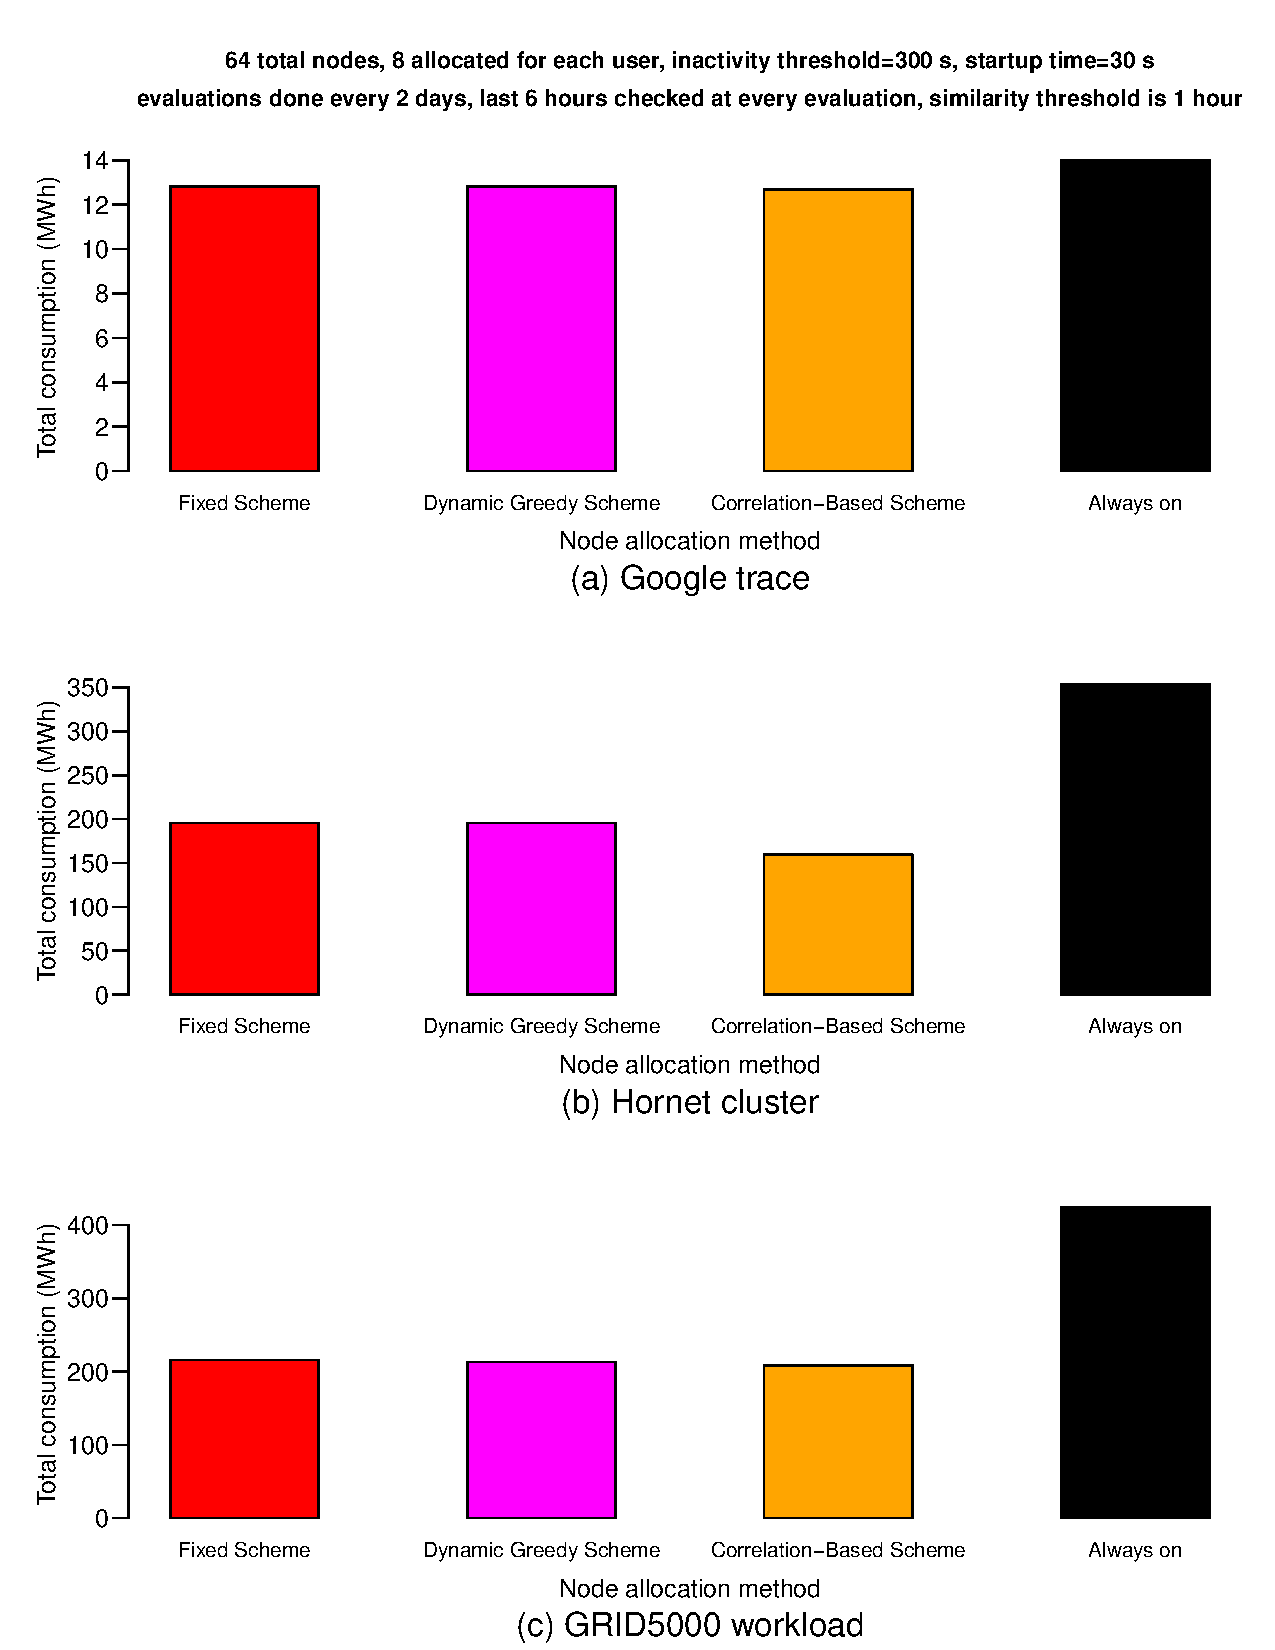
\includegraphics[width=\columnwidth,keepaspectratio]{FIG5.pdf}
\caption{Energy consumption comparison of methods}
\label{bigresult}
\end{figure}

Figure~\ref{bigresult} shows that, for the Google trace any of the methods would deliver the same amount
of energy savings and the percentage of energy savings is 8.4\% at its maximum. Google trace is a highly
I/O intensive workload and there are not many idle periods in the system. As a result, energy savings are
not significant. For Hornet cluster data and GRID5000 workload, we observe that all three workloads save
significant amount of energy. For both of these workloads, we see that Dynamic Greedy scheme does not
improve on energy consumption that much compared to the Fixed scheme. One of the main objectives of the
Dynamic Greedy scheme is to balance load across the storage system. As a result, balancing the load
across the system prevents further energy savings. Correlation-Based scheme provides slightly better energy
savings for GRID5000 workload and much better energy savings for Hornet cluster data. Hornet cluster is mostly
used by researchers working simultaneously on a project which potentially improves the correlation
between storage system users. For Hornet cluster data the energy savings are as high as 55\% and
for GRID5000 workload energy savings are as high as 50.9\%.

\subsection{Fixed Scheme}
We first evaluate the Fixed scheme, where one of the node allocation techniques (balancing, sequential,
random or groups) is chosen and kept active unless manually changed. We calculate the total
energy consumption, load balance and latency per access with 64 total nodes in the system,
where 8 nodes are allocated for each user. Figure~\ref{firstresult} shows how energy consumption, load balance
and latency per access change with each node allocation technique. \textit{Random} node allocation technique is
executed five times and the average result is reported, as it can yield to a different result
at each run. Due to space considerations, we show only the Google trace evaluations of the Fixed scheme,
as other workloads have similar results. 
 
\begin{figure}[!htbp]
\centering
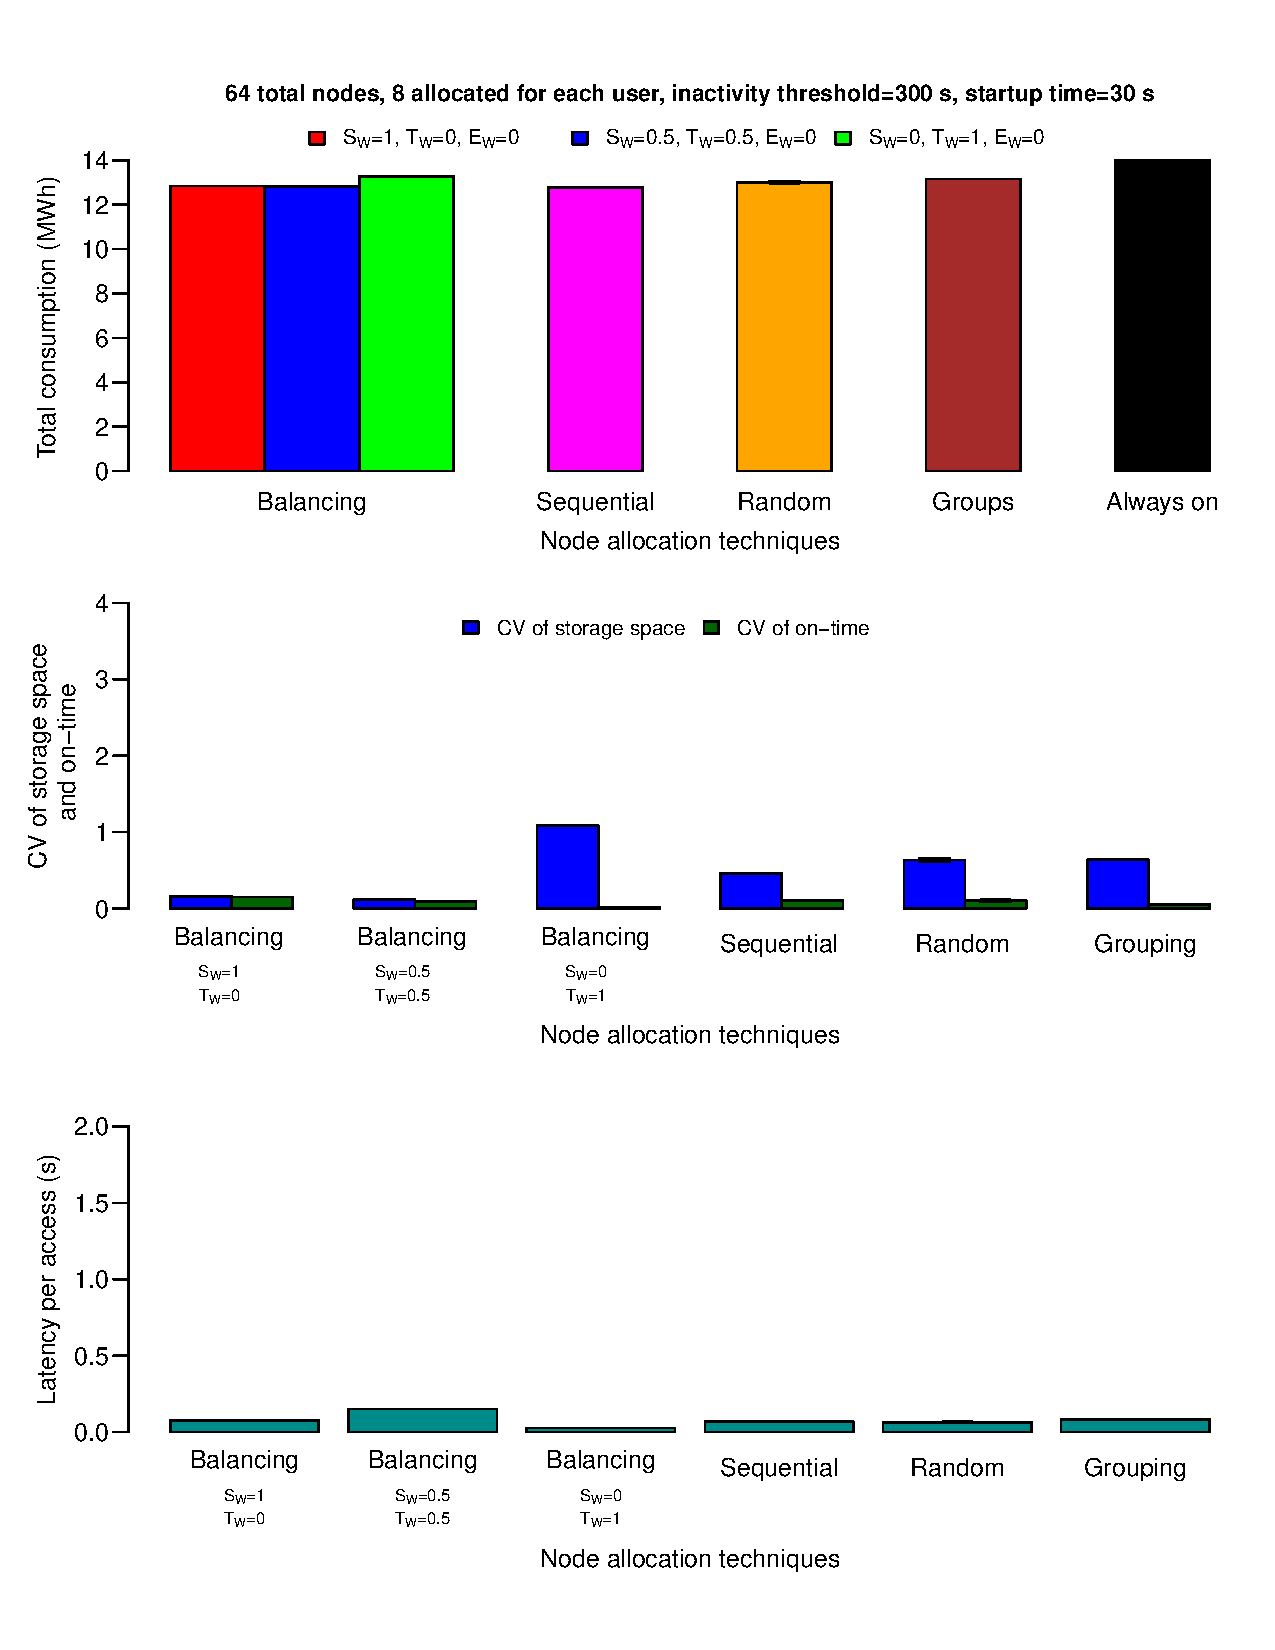
\includegraphics[width=\columnwidth,keepaspectratio]{FIG6.pdf}
\caption{Allocation technique vs energy consumption, load balance and latency per access (Fixed scheme - Google trace)}
\label{firstresult}
\end{figure}

As seen in Figure~\ref{firstresult}, each node allocation technique saves some amount of energy
compared to the stock case where there is no energy saving technique in place (system always on).
The percentage of savings is around 8.4\% for the Google trace. Google trace is highly intensive and as a
result, there are not that many idle periods in this workload. Therefore, energy savings are limited in
such a busy workload.
The amount of energy savings does not
vary much with different techniques. Balancing technique with on-time balancing weight ($T_W$) set to
one consumes slightly more energy compared to other techniques. The primary objective of balancing technique
with on-time balancing weight set to one is to balance the on-time of nodes across the storage system. We found
from the Google trace that majority of the storage system accesses are in the range of couple hundred seconds.
Google trace workload is already balanced initially in terms of node on-time; therefore, balancing technique
with on-time balancing weight set to one does not change the node allocations as much as other techniques do,
resulting in higher energy consumption.

However, the techniques do differ considerably in terms of balancing storage space and on-time. Second sub-plot in
Figure~\ref{firstresult} shows how the coefficient of variation (CV) of storage space and on-time across the storage nodes
vary with different node allocation techniques. As shown in the second sub-plot of Figure~\ref{firstresult}, the
balancing technique with non-zero storage space balancing weight ($S_W$) has smaller CV
of storage space across the storage nodes. Other techniques do not perform that well as their primary objective
is not to balance storage space across the storage nodes.

The balancing technique also performs well for balancing on-time of the storage nodes, as shown in the second sub-plot
of Figure~\ref{firstresult}. Balancing technique with time balancing weight ($T_W$) set to one has the smallest CV
of on-time across the storage nodes as expected.

The third sub-plot in Figure~\ref{firstresult} shows how the latency per access changes with each node allocation technique.
As we have mentioned previously, balancing technique with on-time balancing weight set to one does not change the node
allocations as much as other techniques do. As a result, that technique has the smallest latency per access. On the
other hand, balancing technique with both storage and on-time balancing weight set to 0.5 has the highest energy savings
compared to other techniques; increasing its latency per access. In general, we can see that all techniques have very
close latency per access values, usually around 0.1 seconds. 

\begin{figure}[!htbp]
\centering
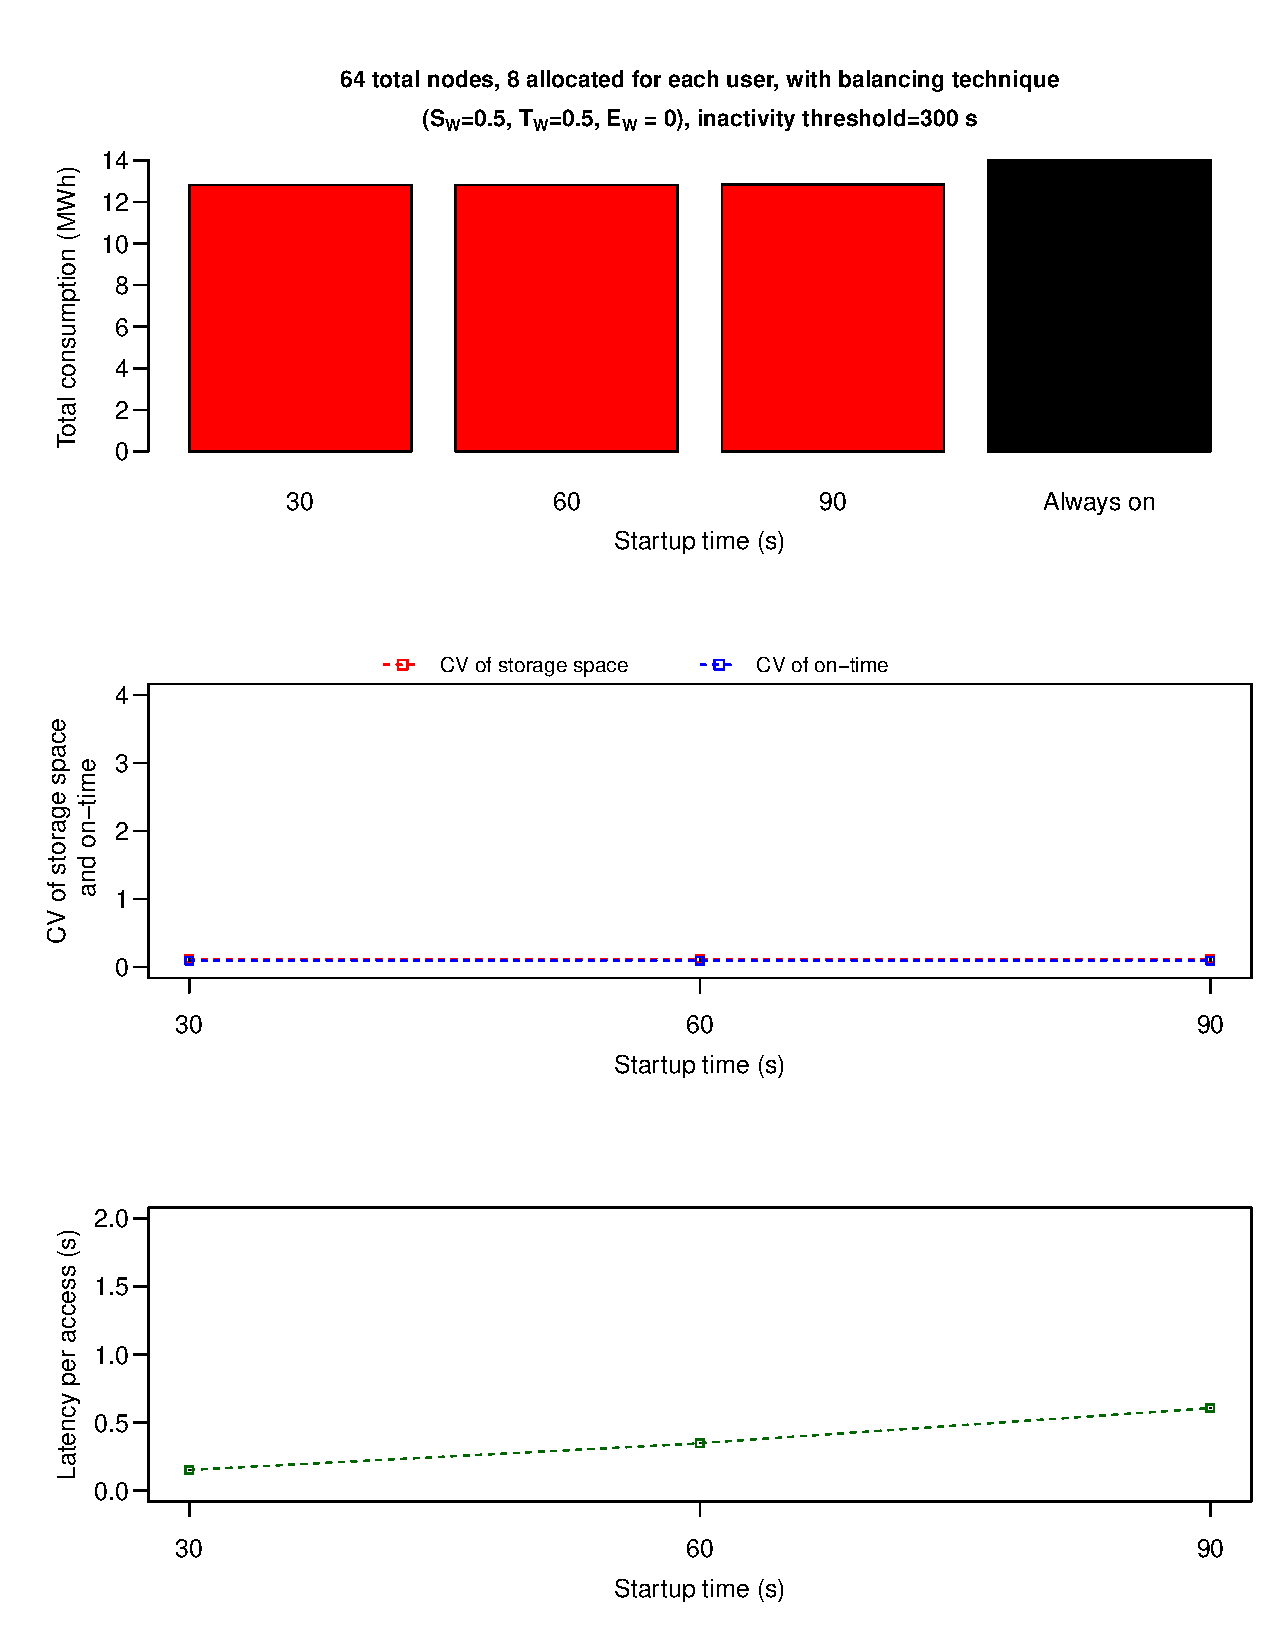
\includegraphics[width=\columnwidth,keepaspectratio]{FIG7.pdf}
\caption{The effect of varying the startup time (Fixed scheme - Google trace)}
\label{secondresult}
\end{figure}

\begin{figure}[!htbp]
\centering
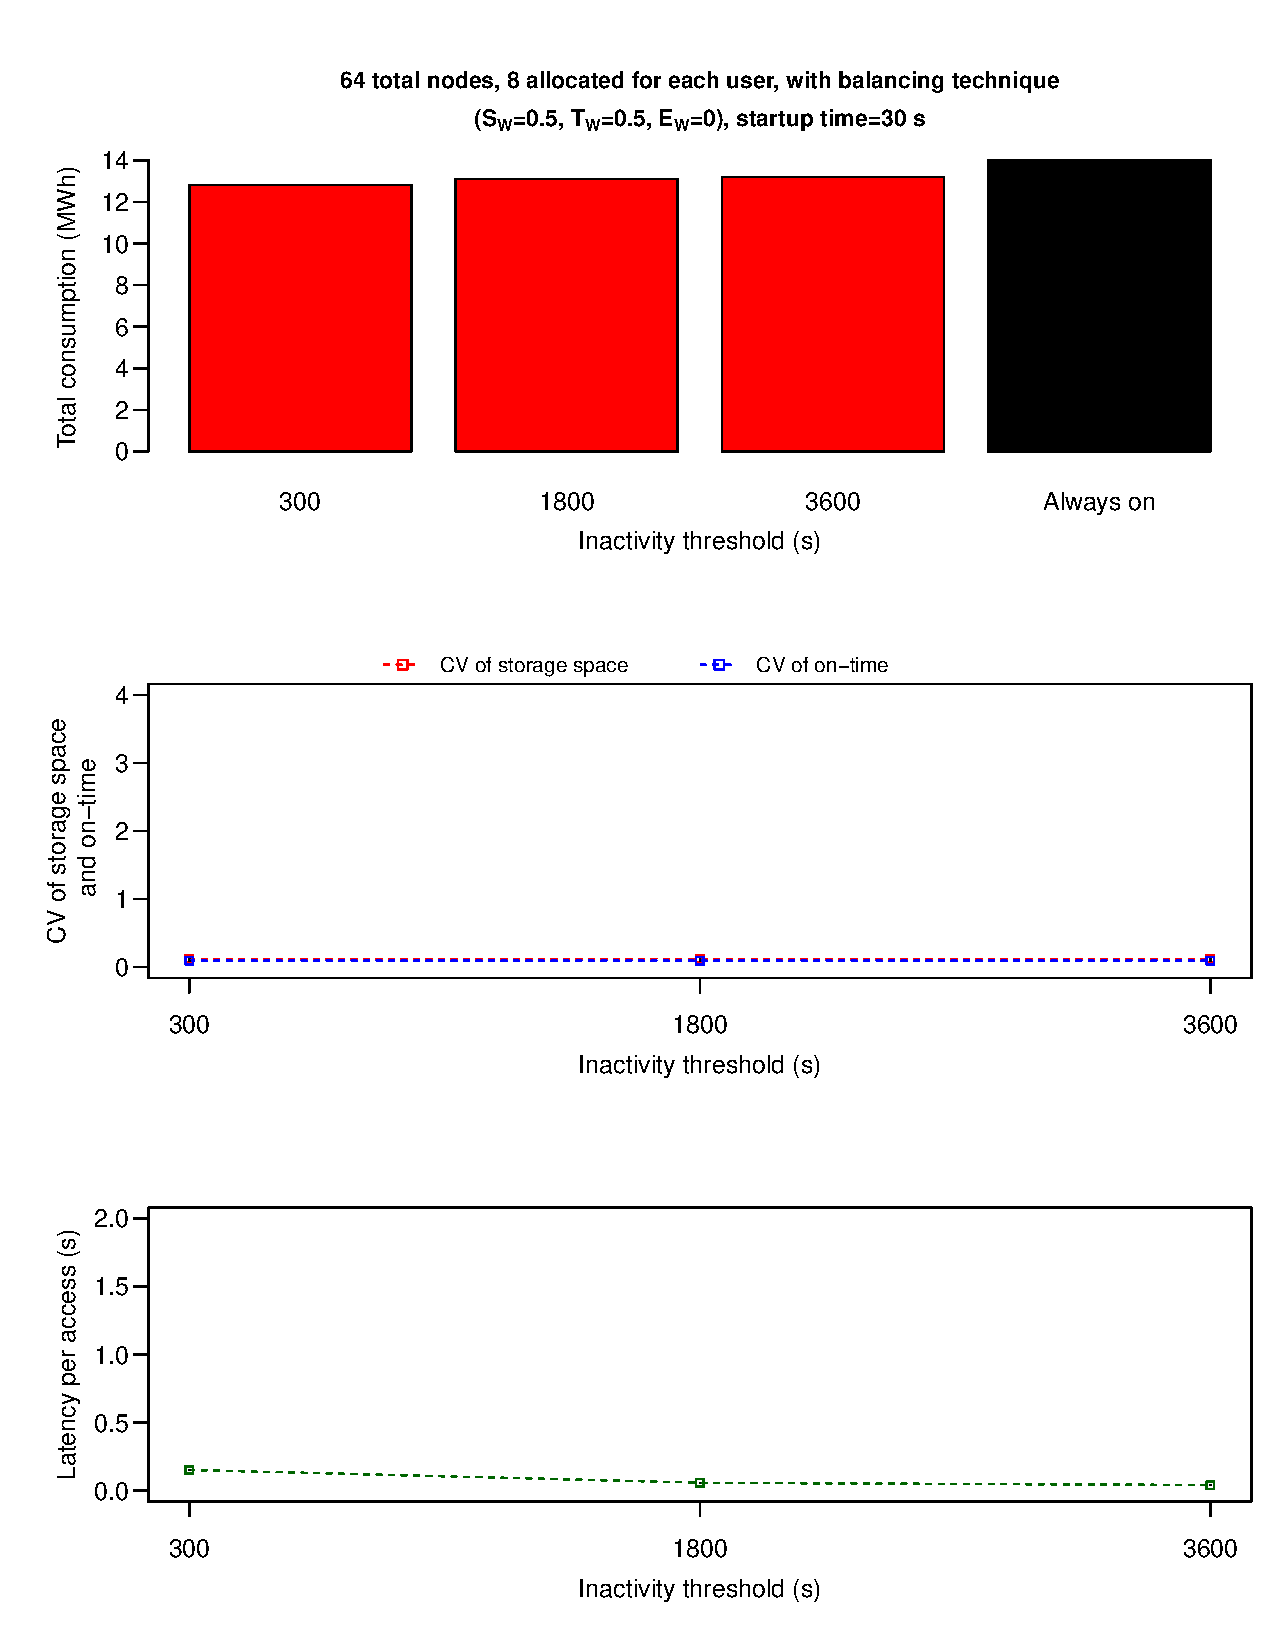
\includegraphics[width=\columnwidth,keepaspectratio]{FIG8.pdf}
\caption{The effect of varying the inactivity threshold (Fixed scheme - Google trace)}
\label{thirdresult}
\end{figure}

We also investigate how the total energy consumption, load balance and latency per access is affected by the changes in
the startup time and inactivity threshold. Figure~\ref{secondresult} shows the total energy consumption,
load balance and latency per access measurements while the startup time is varied between 30, 60 and 90 seconds. Similarly,
Figure~\ref{thirdresult} shows the total energy consumption, load balance and latency per access measurements while the
inactivity threshold is varied between 300, 1800 and 3600 seconds. As each technique is affected similarly by the changes
in the inactivity threshold and startup time, we only present results for the balancing technique with both storage space
and on-time balancing weights ($S_W$ and $T_W$) equal to 0.5 and energy consumption weight ($E_W$) equal to zero.

As we can see in both Figure~\ref{secondresult} and Figure~\ref{thirdresult}, changing the inactivity threshold or the
startup time has nearly no effect on the load balance. Changing the startup time does not affect the energy consumption
either. Figure~\ref{thirdresult} shows that increasing the inactivity threshold causes energy consumption to go up. When
the inactivity threshold is higher, it is less likely for a storage node to be turned-off for being idle longer
than this threshold. This causes the storage node to stay on for longer and consequently increases energy consumption.
Latency per access slightly increases as the startup time is increased. This is expected, since any access that is made
to a turned-off node will wait longer for that node to startup again. On the other hand, as the inactivity threshold is
increased, latency per access slightly decreases. In that case, the storage nodes are kept on for longer due to higher
inactivity threshold; which means that less storage system accesses will be made to a turned-off node.

\subsection{Dynamic Greedy Scheme}
In this section, we evaluate the Dynamic Greedy scheme and find out how effective it is in terms of energy consumption, 
load balance and latency per access. As discussed in Section~\ref{greedy}, \textit{evaluation points} and
\textit{control periods} are two important parameters of the Dynamic Greedy scheme. Dynamic Greedy scheme starts with
one of the four node allocation techniques we proposed (balancing, sequential, random or grouping) and changes between
these techniques at evaluation points, if necessary. We try to understand if the initial technique chosen has any effect
on the energy consumption, load balance or latency. We also analyze the effect of varying evaluation points and
control periods on the energy consumption, load balance and latency per access.

To start with, we test the Dynamic Greedy scheme with varying storage-space, on-time and energy consumption weights
($S_W$, $T_W$ and $E_W$) where the total number of storage nodes in the system is 64 and the number of nodes allocated
for each user is 8, as shown in Figure~\ref{fourthresult}. The evaluations are done every 2 days and the storage
accesses in the last 6 hours are checked. Each measurement is the average of five runs. Due to space considerations, we
show only the Hornet cluster evaluations of the Dynamic Greedy scheme, as other workloads have similar results.

\begin{figure}[!htbp]
\centering
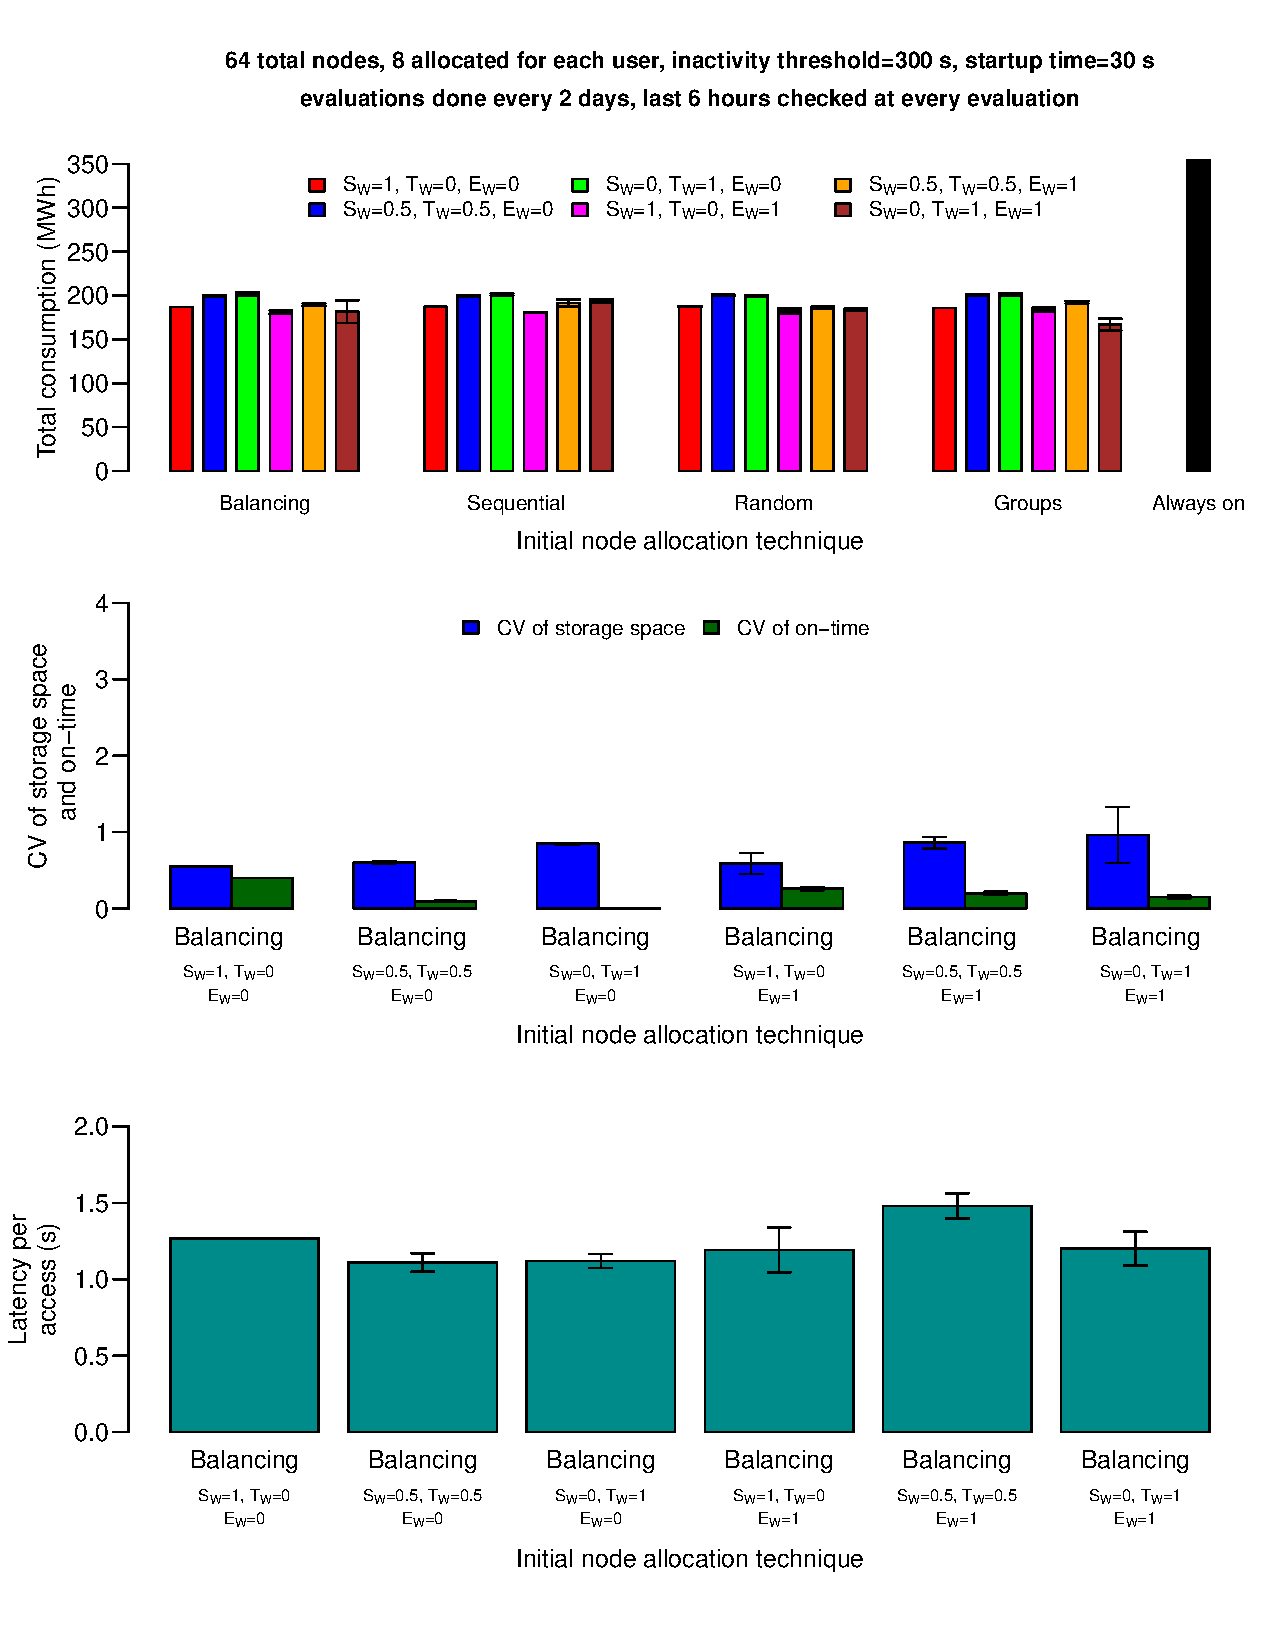
\includegraphics[width=\columnwidth,keepaspectratio]{FIG9.pdf}
\caption{Initial technique vs energy consumption, load balance and latency per access (Dynamic Greedy scheme - Hornet cluster)}
\label{fourthresult}
\end{figure}

Figure~\ref{fourthresult} shows that the Dynamic Greedy scheme saves a considerable amount of energy regardless of
which node allocation technique is chosen initially. The percentage of energy savings are between 43.4\% and 52\%
for varying storage space, on-time and energy weights. Regardless of which technique is initially chosen, we can
see that cases where the energy consumption weight ($E_W$) is set to one consume less energy compared to the cases
where the energy consumption weight is set to zero. Another observation we can make is that the cases where the
on-time balancing weight ($T_W$) is non-zero and energy consumption weight ($E_W$) is set to zero consume more
energy. In the Hornet cluster workload, storage system access lengths vary significantly. As a result,
while trying to balance the on-time across the storage nodes, it is more likely to transfer users from one node
to another. Storage space usage among the users vary as well, though not as much as the access lengths.

In the second sub-plot of Figure~\ref{fourthresult}, we can see how the CVs of storage space and
on-time change when the storage space, on-time and energy consumption weights are varied. Regardless of
which allocation technique is chosen initially (balancing, sequential, random or grouping) the CVs of the
storage space and on-time are similar. Therefore, we only show the results for cases where balancing technique
is the initially chosen technique. We can see that the CV of the storage space is the smallest when the storage space
balancing weight ($S_W$) is set to one, regardless of the energy consumption weight ($E_W$). As the on-time
balancing weight ($T_W$) is increased, the CV of the storage space increases as well. The same holds true
for the CV of the on-time. When the on-time balancing weight ($T_W$) is set to one, the CV of the on-time
is the smallest regardless of the energy consumption weight ($E_W$). As the storage space balancing
weight ($S_W$) is increased, the CV of the on-time increases as well.

We can see how latency per storage access changes with varying storage space, on-time and energy consumption
weights in the third sub-plot of Figure~\ref{fourthresult}. Again, as it does not matter which allocation technique
is initially chosen, we only show the results for cases where the balancing technique is the initially chosen
technique. The latency
measurements are almost the inverse of the energy consumption measurements in the first sub-plot of
Figure~\ref{fourthresult}. In the first sub-plot of Figure~\ref{fourthresult}, we have seen that when the energy
consumption weight ($E_W$) is set to one, the energy consumption goes down. This means that a storage access
will most likely be made on a turned-off node, increasing latency per access. We have also seen in the
first sub-plot of Figure~\ref{fourthresult} that when on-time balancing weight is non-zero and the energy
consumption weight ($E_W$) is set to zero, the energy savings are less. This will in turn
decrease the chance of an access to be made to a turned-off node, decreasing latency per access.

\begin{figure}[!htbp]
\centering
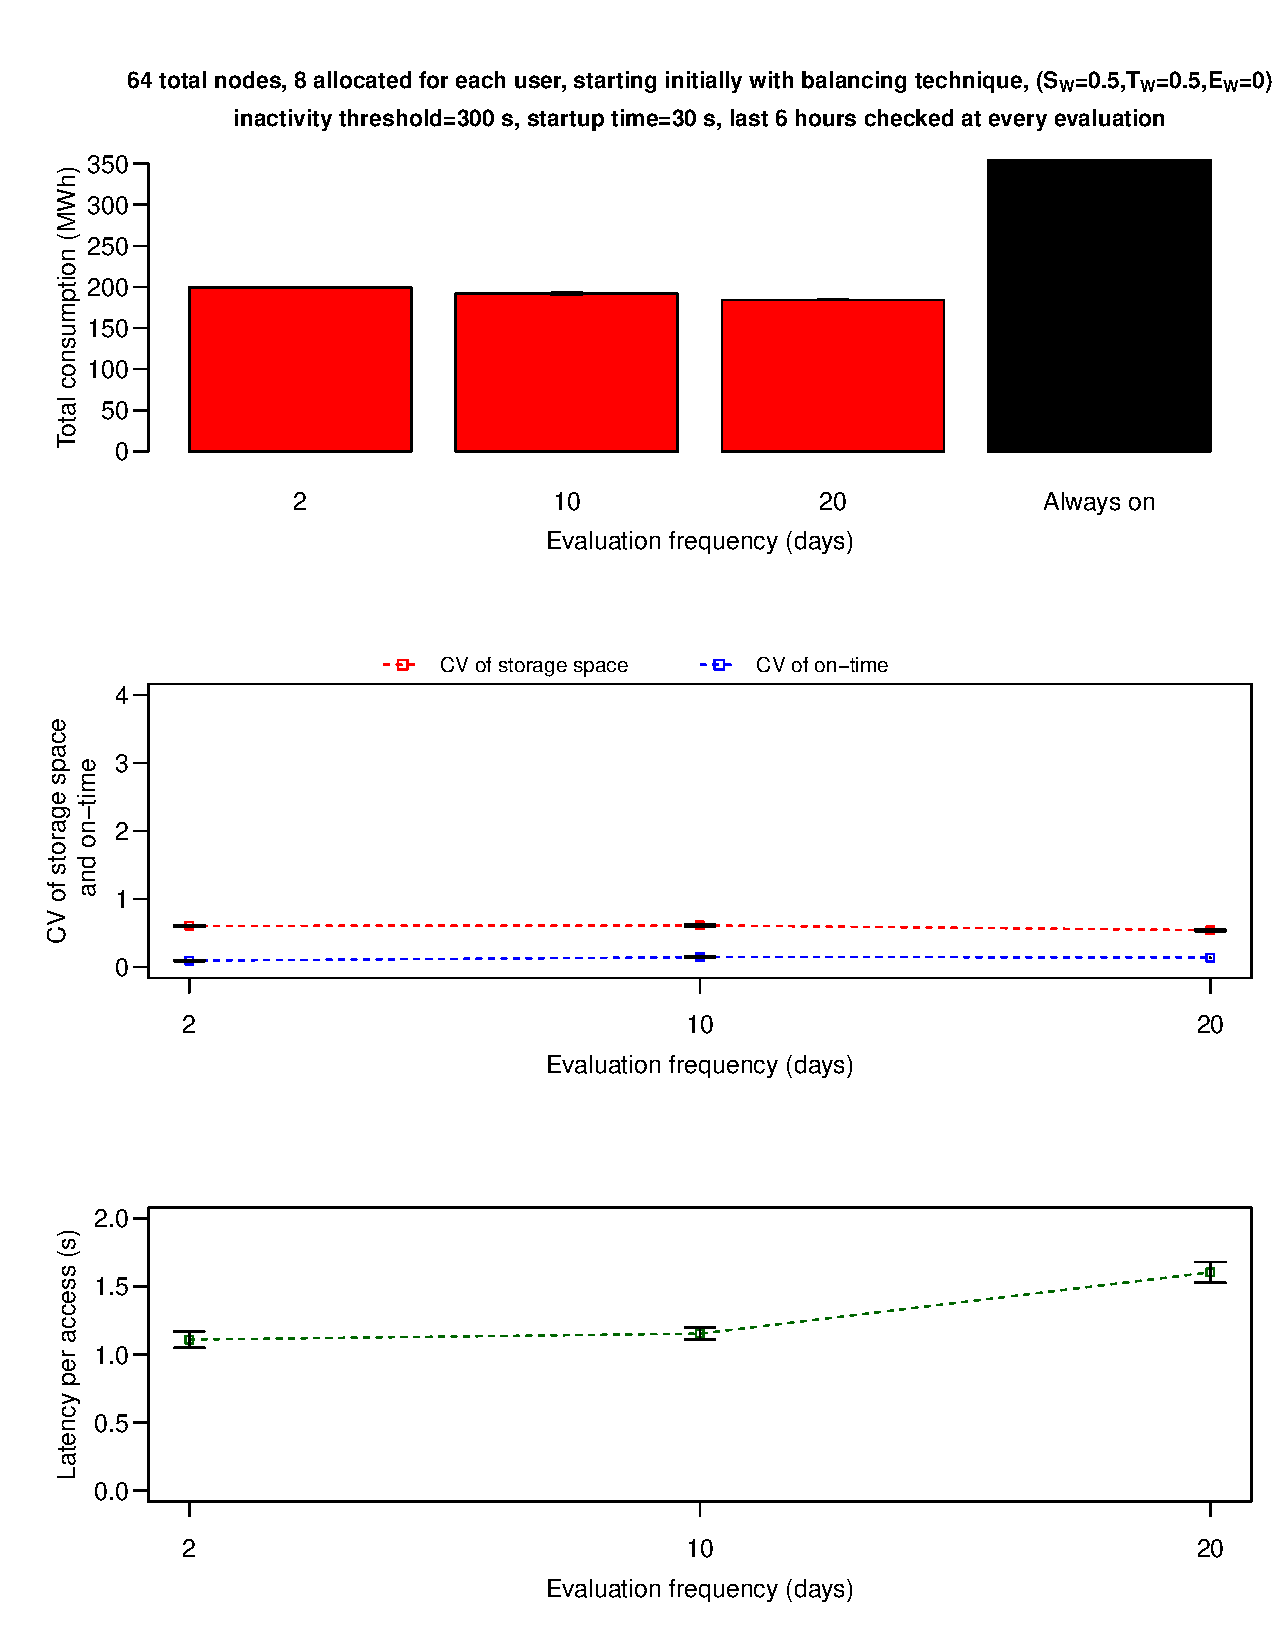
\includegraphics[width=\columnwidth,keepaspectratio]{FIG10.pdf}
\caption{The effect of varying the evaluation frequency (Dynamic Greedy scheme - Hornet cluster)}
\label{fifthresult}
\end{figure}

We now look at the effect of varying the evaluation frequency on the total energy consumption,
load balance and latency per access. The evaluation frequency is varied between 2, 10 and 20 days
and the control period is fixed at 6 hours. Since the initial allocation technique does not change
the results, we initially start with the balancing technique with both storage space and on-time
balancing weights ($S_W$ and $T_W$) set to 0.5 and energy consumption weight ($E_W$) set to zero.
As shown in Figure~\ref{fifthresult}, total energy consumption goes down as the evaluation frequency
becomes longer. When the evaluation frequency is longer, our algorithms have more knowledge about
the state of the storage system. Therefore, more intelligent decisions are made for reducing energy
consumption. We also see that the CVs of the storage space and on-time is almost not affected by
the evaluation frequency. In the third sub-plot of Figure~\ref{fifthresult}, we observe that latency
per access increases as the evaluation frequency becomes longer. This is expected, as longer evaluation
frequency reduces energy consumption by turning off storage nodes more often. 

\begin{figure}[!htbp]
\centering
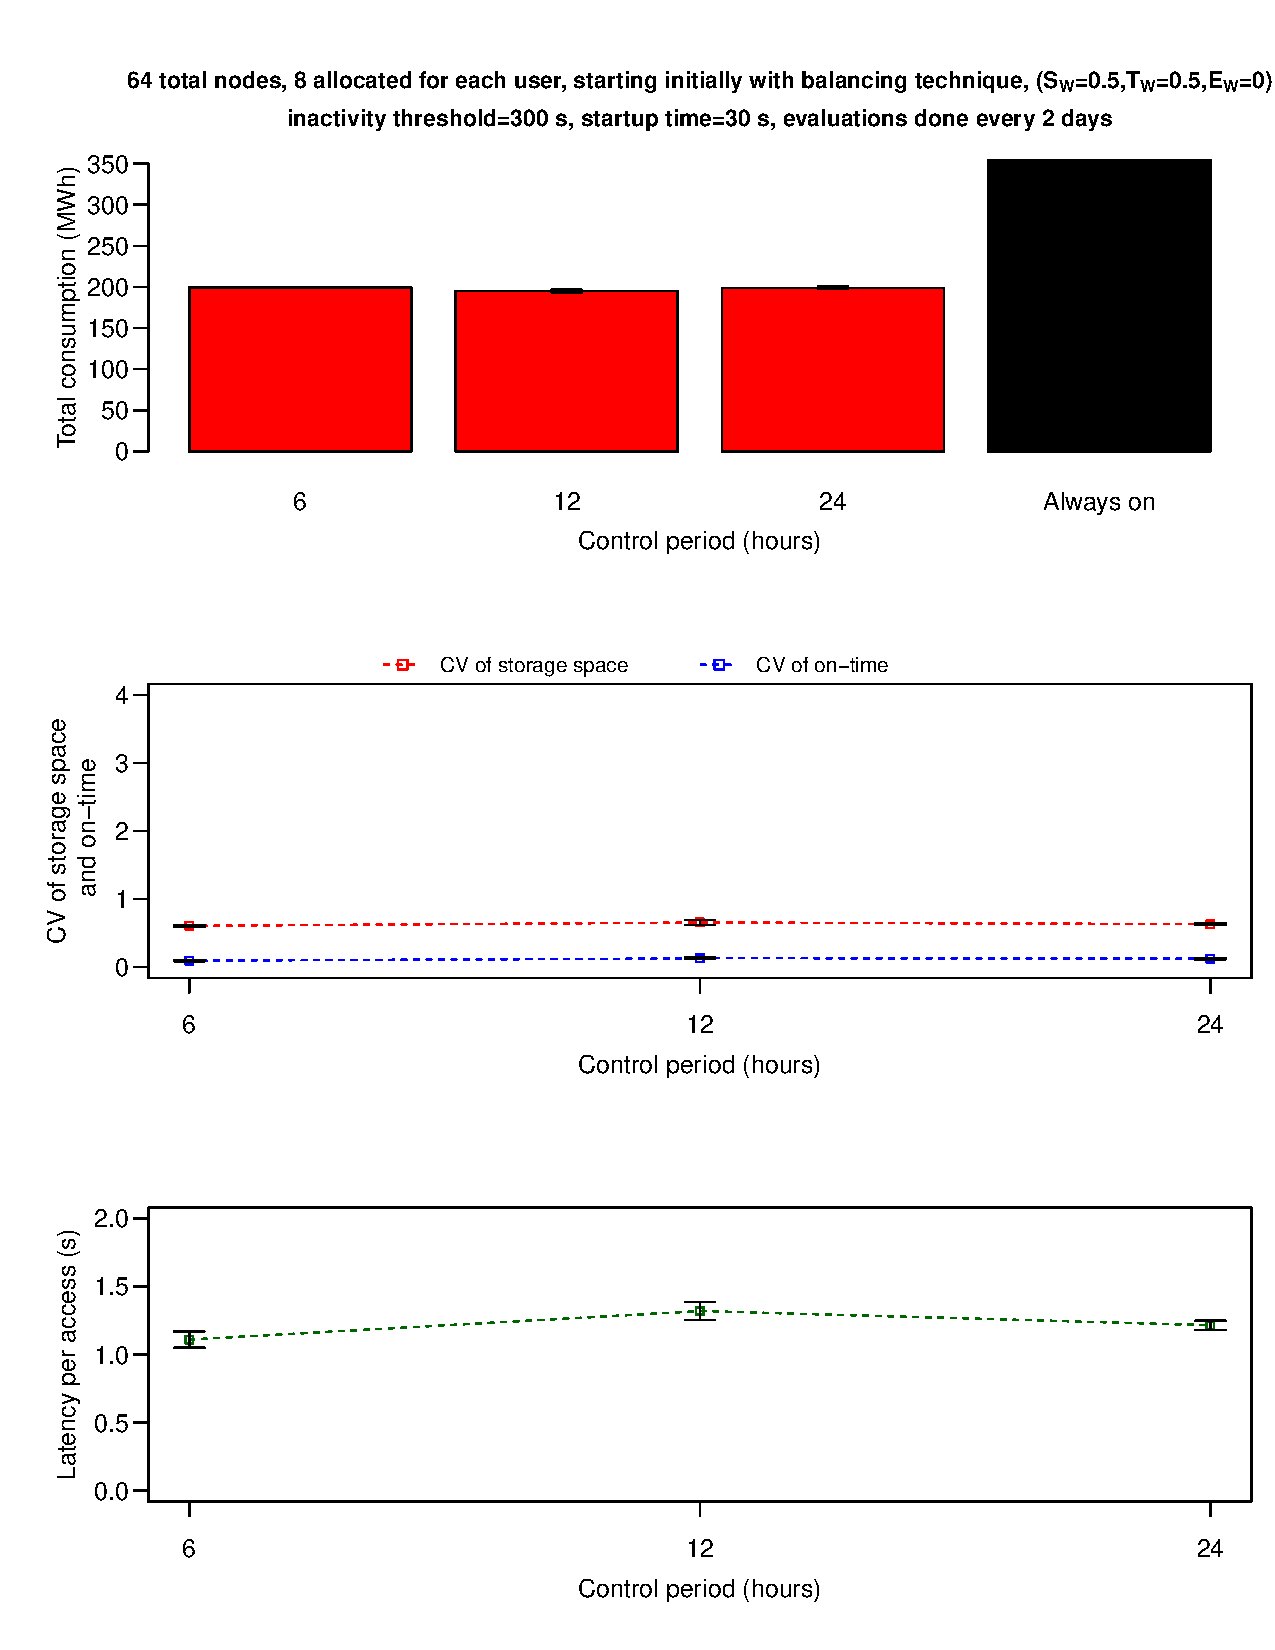
\includegraphics[width=\columnwidth,keepaspectratio]{FIG11.pdf}
\caption{The effect of varying the control period (Dynamic Greedy scheme - Hornet cluster)}
\label{sixthresult}
\end{figure}

Figure~\ref{sixthresult} shows the effect of varying the control period (between 6, 12 and 24 hours)
on the total energy consumption, load balance and latency per access. In this test case the evaluation
frequency is fixed at 2 days. The results in Figure~\ref{sixthresult} indicate that varying the control
period does not affect the total energy consumption, load balance or latency per access.

\subsection{Correlation-Based Scheme}
In this section, we evaluate the Correlation-Based scheme and find out how effective it is in terms of energy consumption,
load balance and latency per access. Correlation-Based scheme starts with one of the four node allocation
techniques (balancing, sequential, random or grouping) similar to the Dynamic Greedy scheme. Unlike the Dynamic
Greedy scheme, it checks the correlations between users at evaluation points and allocates the same storage
nodes for correlated users instead of changing the initial node allocation technique. As a matter of fact,
initial node allocation technique is used if only a user accesses the storage system for the first time.
During the following tests, we also try to understand if the initial technique chosen has any effect on the
energy consumption, load balance or latency per access.

Correlation-Based scheme also has \textit{evaluation point} and \textit{control period} parameters. We have
already shown the effect of varying these two parameters for the Dynamic Greedy scheme; therefore, we are not
repeating the same tests for Correlation-Based scheme. \textit{Similarity threshold} is a parameter that
is unique to the Correlation-Based scheme. We look at the effect of this parameter on the energy consumption,
load balance and latency per access as well.

To start with, we test the Correlation-Based scheme with different initial techniques, where the total number of
storage nodes in the system is 64 and the number of nodes allocated for each user is 8, as shown in 
Figure~\ref{seventhresult}. The evaluations are done every 2 days and the storage accesses in the last 6 hours
are checked. Each measurement is the average of five runs. Since energy consumption weight is not important
in Correlation-Based scheme, it is fixed at zero in this test case. Due to space considerations, we
show only the GRID5000 workload evaluations of the Correlation-Based scheme, as other workloads have similar
results.

\begin{figure}[!htbp]
\centering
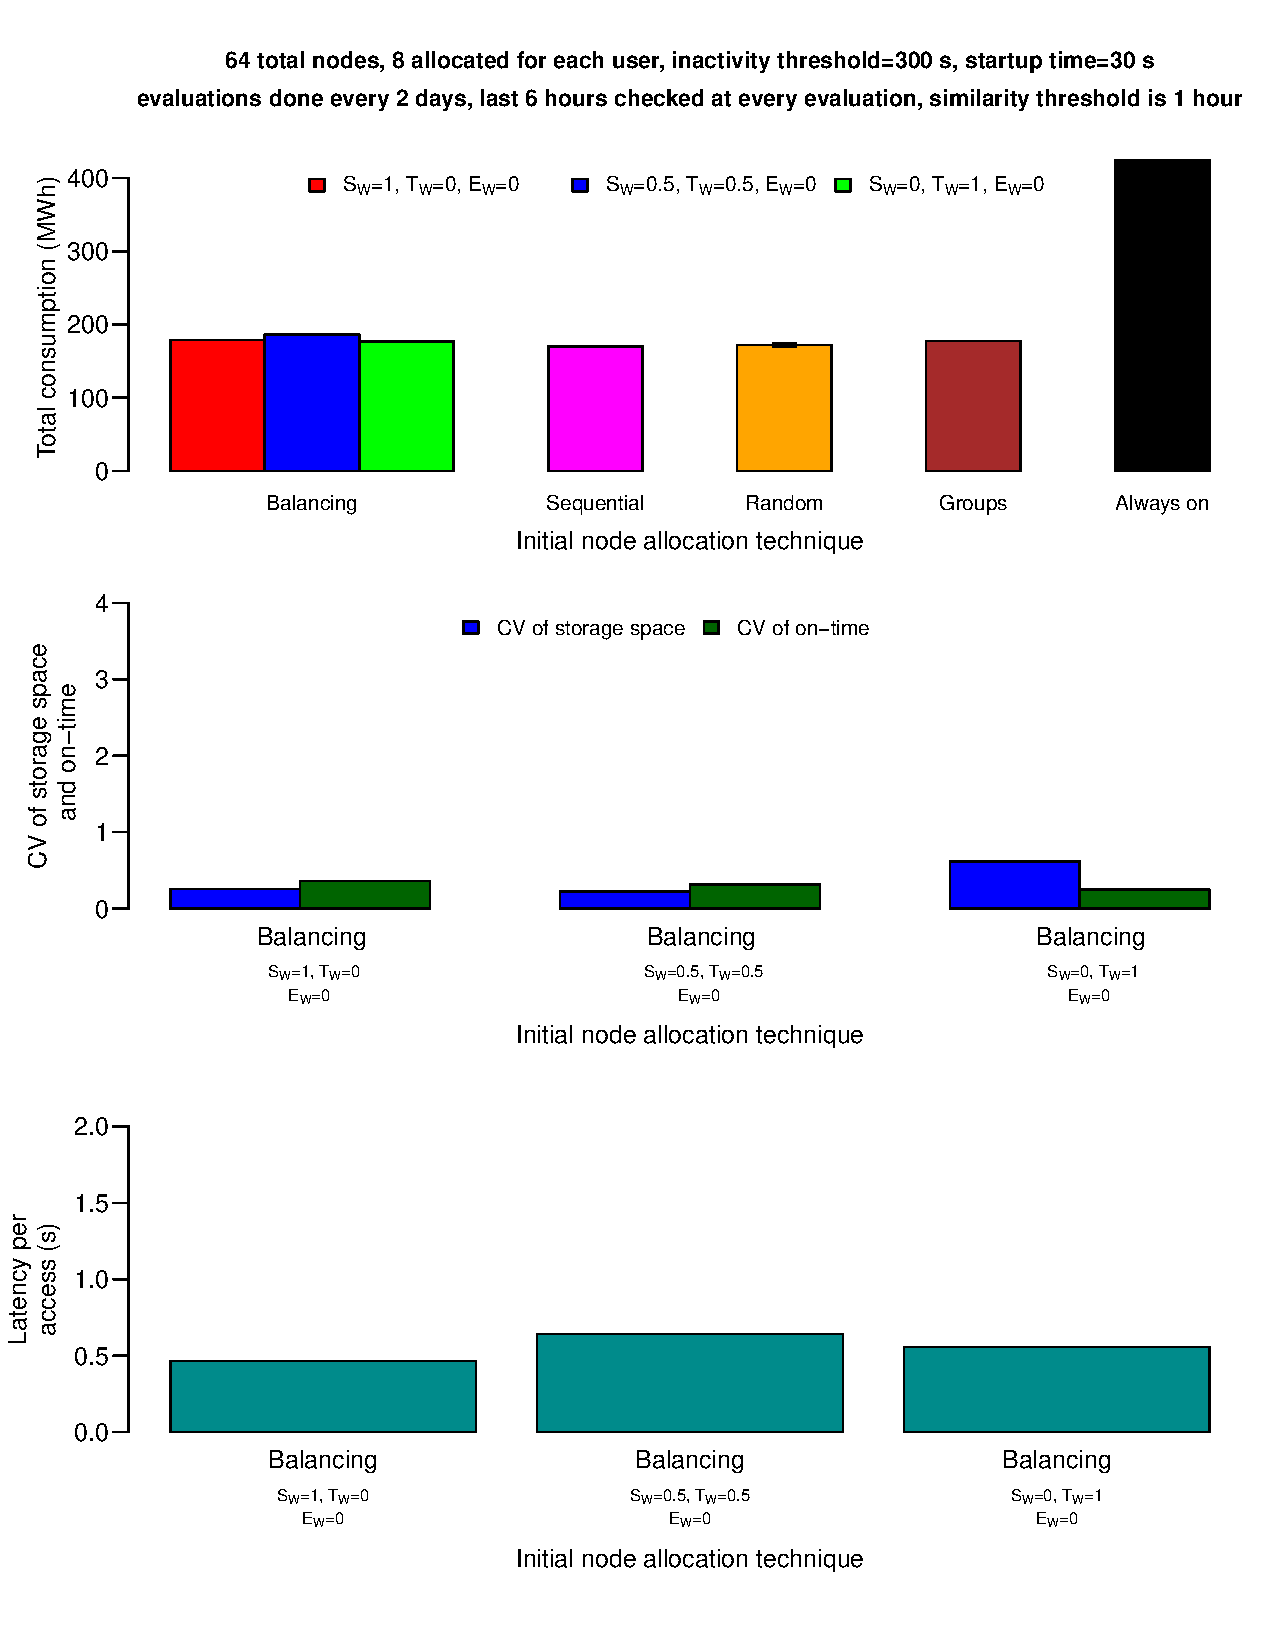
\includegraphics[width=\columnwidth,keepaspectratio]{FIG12.pdf}
\caption{Initial technique vs energy consumption, load balance and latency (Correlation-Based scheme -
 GRID5000 workload)}
\label{seventhresult}
\end{figure}

Figure~\ref{seventhresult} shows that Correlation-Based Scheme saves more than half of the energy consumed
in the stock case regardless of the initial node allocation technique. The percentage of energy savings
are as high as 60\%. We observe that the initial technique chosen does not have a significant effect on
the energy consumption.

The CVs of the storage space and on-time are shown in the second sub-plot of Figure~\ref{seventhresult}.
As the initial technique chosen for the Correlation-Based scheme does not really matter, we show
results for the balancing technique with varying storage-space and on-time balancing weights. As the
storage space balancing weight ($S_W$) is increased, the CV of the storage space
decreases. The same is true for on-time.

The third sub-plot in Figure~\ref{seventhresult} shows how latency per access is affected when the initial
technique is balancing with varying storage-space and on-time balancing weights. In GRID5000 workload, the
storage space usage of users are close to each other. Therefore balancing technique with storage-space
balancing weight set to one will not effect the node allocations as much as other techniques do. We observed
that GRID5000 workload havs accesses of varying lengths, particularly
until the first evaluation point. As a result, if both the storage space balancing and on-time weight are set
to 0.5, then the algorithm will not try to break already balanced storage-space distribution, while at the
same time trying to balance on-time. This will in turn result in more transfers and consequently more latency.
This feature of the GRID5000 workload is similar to that of Google trace in Figure~\ref{firstresult}, except
that Google trace had varying storage space usage among the users where access lenghts did not vary that much.

\begin{figure}[!htbp]
\centering
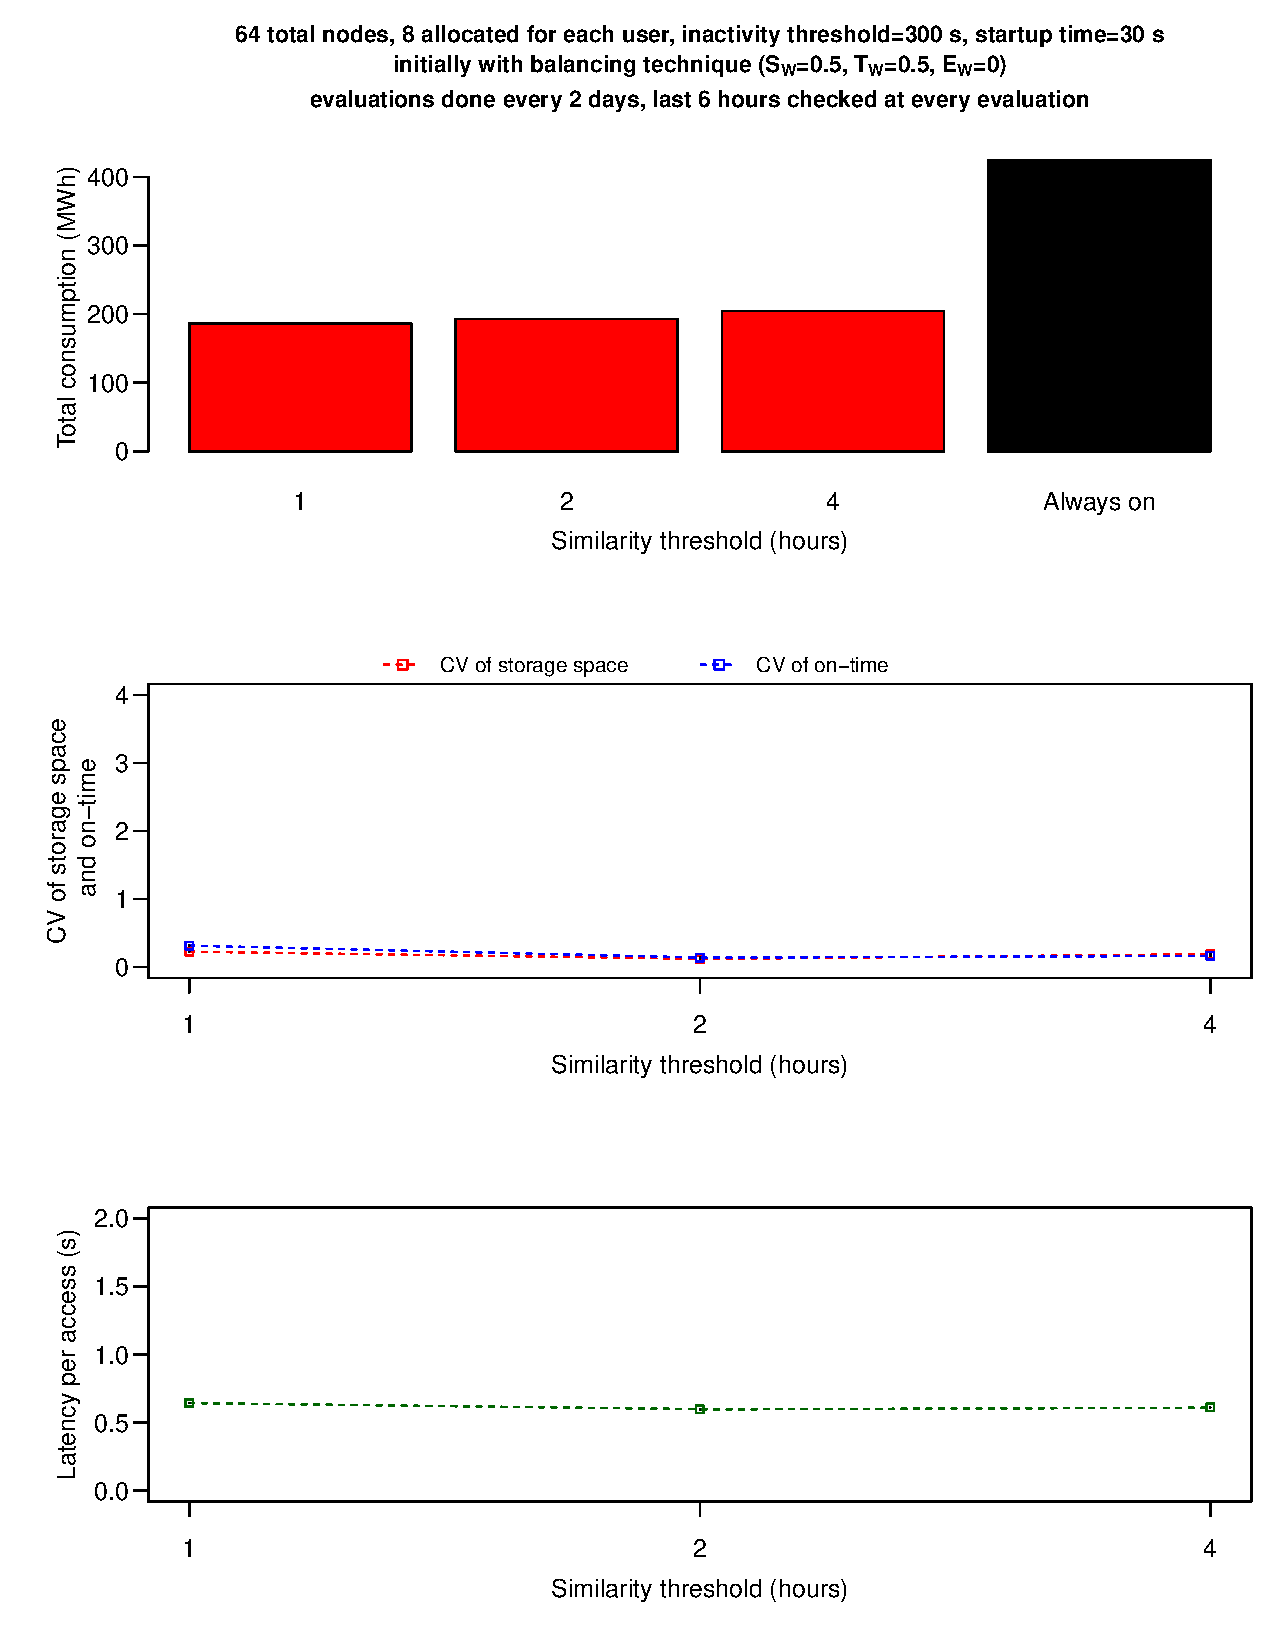
\includegraphics[width=\columnwidth,keepaspectratio]{FIG13.pdf}
\caption{The effect of varying the similarity threshold (Correlation-Based scheme - GRID5000 workload)}
\label{eightthresult}
\end{figure} 

Figure~\ref{eightthresult} shows the effect of varying the similarity threshold on the total energy
consumption, load balancing and latency per access. Evaluations are done every 2 days and the last 6 hours
are checked at every evaluation. Balancing technique with both storage space and on-time balancing
weights set to 0.5 is used initially. Similar to the inactivity threshold, varying the
similarity threshold has almost no effect on the standard devations of the storage space and on-time
or latency per access. When the similarity threshold is increased, total energy consumption
increases slightly. The higher the similarity threshold is, the less likely it is to find correlated
users. As a result, energy consumption goes up with higher similarity threshold.

\subsection{Validating Mathematical Model}
\label{validate_model}
We have validated the mathematical model presented in Section~\ref{model} against the
experimental results of our approach using data from Hornet HPC system. We can estimate the energy
consumption, load balancing and latency per access values for each workload
by using the mathematical model presented in Section~\ref{model}. We validate
the mathematical model using the subset of test parameters as shown in
Table~\ref{tbl:validate_params}.
For brevity, we show only the Hornet data, though the other workloads show similar results.
For the Hornet data that we show here for this validation, we have primarily used a Generalized
Extreme Value interjob arrival model - i.e.
$F(t) = e^{-g(t)},\ \ where\ \ g(t)\ \ =\ \ [{1 + (\frac{t - \mu}{\sigma}) * \xi}]^{\frac{-1}{\xi}}$
and $\xi,\ \ \mu$ and $\sigma$ are distribution parameters.

\begin{table}[!htbp]
 \begin{center}
  \begin{tabular}{|l|l|} \hline
Test Parameter & Values \\ \hline
Total number of nodes          & 64 \\ \hline
Number of nodes allocated        & 8 \\
for each user              & \\ \hline
Allocation methods           & Fixed, Dynamic Greedy, Correlation-Based \\ \hline
Low-energy mode             & Turn Off \\ \hline
Inactivity threshold          & 300 s \\ \hline
Startup time              & 30 s \\ \hline
Similarity threshold          & 3600 s \\ \hline
Storage space and on-time        & 0.5, 0.5, 0 \\
balancing weights            & \\ \hline
Power consumption per node       & 300 W \\ \hline
Workloads                        & Hornet \\ \hline
  \end{tabular}
 \end{center}
 \caption{Mathematical Model Validation Parameters}
 \label{tbl:validate_params}
\end{table}

Tables~\ref{tbl:validate_results_fixed},~\ref{tbl:validate_results_dynamic} and ~\ref{tbl:validate_results_corr} show
that the mathematical model we presented is able to estimate the test result parameters (CV of storage space, CV of on-time
, energy cost and latency per access) accurately in most
cases. The storage space usage of a user per storage node does not change over time; therefore, the chance of
estimating it accurately is high. Our model estimates on-time value and energy consumption of each storage node accurately
as well, as estimating them involves all of the parameters captured by our model except storage space usage.
Latency per access is highly dependent on the arrival rate of \textit{interarrivals} and our model does the best attempt to
capture these interarrivals in order to estimate the latency per access.

\begin{table}[!htbp]
 \begin{center}
 \resizebox{\textwidth}{!}{%
  \begin{tabular}{lcccccccc} \hline
\multicolumn{1}{|c}{} & \multicolumn{4}{c|}{Balancing} & \multicolumn{4}{c|}{Sequential}\\ \hline
\multicolumn{1}{|c}{} & \multicolumn{1}{|c}{Storage} & \multicolumn{1}{c}{On-time} & \multicolumn{1}{c}{Energy} & \multicolumn{1}{c|}{Latency per} & \multicolumn{1}{c}{Storage} & \multicolumn{1}{c}{On-time} & \multicolumn{1}{c}{Energy} & \multicolumn{1}{c|}{Latency per} \\
\multicolumn{1}{|c}{} & \multicolumn{1}{|c}{CV} & \multicolumn{1}{c}{CV} & \multicolumn{1}{c}{cost (MWh)} & \multicolumn{1}{c|}{access (s)} & \multicolumn{1}{c}{CV} & \multicolumn{1}{c}{CV} & \multicolumn{1}{c}{cost (MWh)} & \multicolumn{1}{c|}{access (s)} \\ \hline
\multicolumn{1}{|l|}{Simulation} & 0.539 & 0.312 & 195.65 & \multicolumn{1}{c|}{1.0348} & 0.757 & 0.382 & 181.01 & \multicolumn{1}{c|}{1.1833} \\ 
\multicolumn{1}{|l|}{Model} & 0.543 & 0.3145 & 195.62 & \multicolumn{1}{c|}{1.1657} & 0.7628 & 0.3849 & 180.93 & \multicolumn{1}{c|}{1.1669} \\
\multicolumn{1}{|l|}{Error} & 0.74\% & 0.80\% & 0.02\% & \multicolumn{1}{c|}{12.65\%} & 0.77\% & 0.76\% & 0.04\% & \multicolumn{1}{c|}{1.39\%} \\ \hline
& & & & & & & & \\ \hline
\multicolumn{1}{|c}{} & \multicolumn{4}{c|}{Random} & \multicolumn{4}{c|}{Groups}\\ \hline
\multicolumn{1}{|c}{} & \multicolumn{1}{|c}{Storage} & \multicolumn{1}{c}{On-time} & \multicolumn{1}{c}{Energy} & \multicolumn{1}{c|}{Latency per} & \multicolumn{1}{c}{Storage} & \multicolumn{1}{c}{On-time} & \multicolumn{1}{c}{Energy} & \multicolumn{1}{c|}{Latency per} \\
\multicolumn{1}{|c}{} & \multicolumn{1}{|c}{CV} & \multicolumn{1}{c}{CV} & \multicolumn{1}{c}{cost (MWh)} & \multicolumn{1}{c|}{access (s)} & \multicolumn{1}{c}{CV} & \multicolumn{1}{c}{CV} & \multicolumn{1}{c}{cost (MWh)} & \multicolumn{1}{c|}{access (s)} \\ \hline
\multicolumn{1}{|l|}{Simulation} & 0.9 & 0.394 & 179.81 & \multicolumn{1}{c|}{1.5673} & 1.129 & 0.351 & 183.78 & \multicolumn{1}{c|}{1.0367} \\ 
\multicolumn{1}{|l|}{Model} & 0.9069 & 0.3973 & 179.753 & \multicolumn{1}{c|}{1.2496} & 1.1381 & 0.3539 & 183.711 & \multicolumn{1}{c|}{1.0539} \\
\multicolumn{1}{|l|}{Error} & 0.77\% & 0.84\% & 0.03\% & \multicolumn{1}{c|}{20.27\%} & 0.81\% & 0.83\% & 0.04\% & \multicolumn{1}{c|}{1.66\%} \\ \hline
  \end{tabular}}
 \end{center}
 \caption{Mathematical Model Validation Results for Fixed Scheme}
 \label{tbl:validate_results_fixed}
\end{table}

\begin{table}[!htbp]
 \begin{center}
 \resizebox{\textwidth}{!}{%
  \begin{tabular}{lcccccccc} \hline
\multicolumn{1}{|c}{} & \multicolumn{4}{c|}{Starts with Balancing} & \multicolumn{4}{c|}{Starts with Sequential}\\ \hline
\multicolumn{1}{|c}{} & \multicolumn{1}{|c}{Storage} & \multicolumn{1}{c}{On-time} & \multicolumn{1}{c}{Energy} & \multicolumn{1}{c|}{Latency per} & \multicolumn{1}{c}{Storage} & \multicolumn{1}{c}{On-time} & \multicolumn{1}{c}{Energy} & \multicolumn{1}{c|}{Latency per} \\
\multicolumn{1}{|c}{} & \multicolumn{1}{|c}{CV} & \multicolumn{1}{c}{CV} & \multicolumn{1}{c}{cost (MWh)} & \multicolumn{1}{c|}{access (s)} & \multicolumn{1}{c}{CV} & \multicolumn{1}{c}{CV} & \multicolumn{1}{c}{cost (MWh)} & \multicolumn{1}{c|}{access (s)} \\ \hline
\multicolumn{1}{|l|}{Simulation} & 0.605 & 0.0932 & 199.36 & \multicolumn{1}{c|}{1.11008} & 0.6186 & 0.0956 & 199.273 & \multicolumn{1}{c|}{1.12687} \\
\multicolumn{1}{|l|}{Model} & 0.6031 & 0.1006 & 199.913 & \multicolumn{1}{c|}{1.0424} & 0.6142 & 0.1 & 200.254 & \multicolumn{1}{c|}{0.9944} \\
\multicolumn{1}{|l|}{Error} & 0.31\% & 7.94\% & 0.28\% & \multicolumn{1}{c|}{6.1\%} & 0.71\% & 4.6\% & 0.49\% & \multicolumn{1}{c|}{11.76\%} \\ \hline
& & & & & & & & \\ \hline
\multicolumn{1}{|c}{} & \multicolumn{4}{c|}{Starts with Random} & \multicolumn{4}{c|}{Starts with Groups}\\ \hline
\multicolumn{1}{|c}{} & \multicolumn{1}{|c}{Storage} & \multicolumn{1}{c}{On-time} & \multicolumn{1}{c}{Energy} & \multicolumn{1}{c|}{Latency per} & \multicolumn{1}{c}{Storage} & \multicolumn{1}{c}{On-time} & \multicolumn{1}{c}{Energy} & \multicolumn{1}{c|}{Latency per} \\
\multicolumn{1}{|c}{} & \multicolumn{1}{|c}{CV} & \multicolumn{1}{c}{CV} & \multicolumn{1}{c}{cost (MWh)} & \multicolumn{1}{c|}{access (s)} & \multicolumn{1}{c}{CV} & \multicolumn{1}{c}{CV} & \multicolumn{1}{c}{cost (MWh)} & \multicolumn{1}{c|}{access (s)} \\ \hline
\multicolumn{1}{|l|}{Simulation} & 0.614 & 0.0926 & 200.199 & \multicolumn{1}{c|}{1.14529} & 0.63 & 0.086 & 200.558 & \multicolumn{1}{c|}{1.09082} \\
\multicolumn{1}{|l|}{Model} & 0.6092 & 0.0923 & 199.577 & \multicolumn{1}{c|}{1.022} & 0.6382 & 0.08 & 201.176 & \multicolumn{1}{c|}{1.0311} \\
\multicolumn{1}{|l|}{Error} & 0.78\% & 0.32\% & 0.31\% & \multicolumn{1}{c|}{10.76\%} & 1.3\% & 6.98\% & 0.31\% & \multicolumn{1}{c|}{5.47\%} \\ \hline
  \end{tabular}}
 \end{center}
 \caption{Mathematical Model Validation Results for Dynamic Greedy Scheme}
 \label{tbl:validate_results_dynamic}
\end{table}

\begin{table}[!htbp]
 \begin{center}
 \resizebox{\textwidth}{!}{%
  \begin{tabular}{lcccccccc} \hline
\multicolumn{1}{|c}{} & \multicolumn{4}{c|}{Starts with Balancing} & \multicolumn{4}{c|}{Starts with Sequential}\\ \hline
\multicolumn{1}{|c}{} & \multicolumn{1}{|c}{Storage} & \multicolumn{1}{c}{On-time} & \multicolumn{1}{c}{Energy} & \multicolumn{1}{c|}{Latency per} & \multicolumn{1}{c}{Storage} & \multicolumn{1}{c}{On-time} & \multicolumn{1}{c}{Energy} & \multicolumn{1}{c|}{Latency per} \\
\multicolumn{1}{|c}{} & \multicolumn{1}{|c}{CV} & \multicolumn{1}{c}{CV} & \multicolumn{1}{c}{cost (MWh)} & \multicolumn{1}{c|}{access (s)} & \multicolumn{1}{c}{CV} & \multicolumn{1}{c}{CV} & \multicolumn{1}{c}{cost (MWh)} & \multicolumn{1}{c|}{access (s)} \\ \hline
\multicolumn{1}{|l|}{Simulation} & 2.059 & 0.35 & 120.842 & \multicolumn{1}{c|}{1.27998} & 2.108 & 0.671 & 105.857 & \multicolumn{1}{c|}{1.27017} \\
\multicolumn{1}{|l|}{Model} & 2.0755 & 0.3523 & 120.798 & \multicolumn{1}{c|}{1.5492} & 2.1244 & 0.676 & 105.826 & \multicolumn{1}{c|}{1.2532} \\
\multicolumn{1}{|l|}{Error} & 0.80\% & 0.66\% & 0.04\% & \multicolumn{1}{c|}{21.03\%} & 0.78\% & 0.75\% & 0.03\% & \multicolumn{1}{c|}{1.34\%} \\ \hline
& & & & & & & & \\ \hline
\multicolumn{1}{|c}{} & \multicolumn{4}{c|}{Starts with Random} & \multicolumn{4}{c|}{Starts with Groups}\\ \hline
\multicolumn{1}{|c}{} & \multicolumn{1}{|c}{Storage} & \multicolumn{1}{c}{On-time} & \multicolumn{1}{c}{Energy} & \multicolumn{1}{c|}{Latency per} & \multicolumn{1}{c}{Storage} & \multicolumn{1}{c}{On-time} & \multicolumn{1}{c}{Energy} & \multicolumn{1}{c|}{Latency per} \\
\multicolumn{1}{|c}{} & \multicolumn{1}{|c}{CV} & \multicolumn{1}{c}{CV} & \multicolumn{1}{c}{cost (MWh)} & \multicolumn{1}{c|}{access (s)} & \multicolumn{1}{c}{CV} & \multicolumn{1}{c}{CV} & \multicolumn{1}{c}{cost (MWh)} & \multicolumn{1}{c|}{access (s)} \\ \hline
\multicolumn{1}{|l|}{Simulation} & 2.056 & 0.638 & 103.395 & \multicolumn{1}{c|}{1.36857} & 2.052 & 0.835 & 107.887 & \multicolumn{1}{c|}{1.30135} \\
\multicolumn{1}{|l|}{Model} & 2.072 & 0.6427 & 103.381 & \multicolumn{1}{c|}{1.5413} & 2.0678 & 0.842 & 107.851 & \multicolumn{1}{c|}{1.249} \\
\multicolumn{1}{|l|}{Error} & 0.78\% & 0.74\% & 0.01\% & \multicolumn{1}{c|}{12.62\%} & 0.77\% & 0.84\% & 0.03\% & \multicolumn{1}{c|}{4.02\%} \\ \hline
  \end{tabular}}
 \end{center}
 \caption{Mathematical Model Validation Results for Correlation-Based Scheme}
 \label{tbl:validate_results_corr}
\end{table}

In this section, we first present experimental simulation results and
then validate the mathematical model presented in Section~\ref{model}.

\subsection{Experimental Setup}
In order to quantify the impact of our energy conservation methods,
we use various workloads that approximate usage in a cloud storage
system. The three workloads come from Google, the University of
Connecticut Hornet HPC system, and the GRID5000 platform. These workloads
are described in more detail below. The jobs in these workloads
are tied to users and each job is assumed to use the storage system equally.

\subsubsection{Workloads}
\paragraph{Google Trace}
The Google Trace is a log of jobs that are run in Google's cloud
system~\cite{clusterdata:Wilkes2011}. This trace has 29 days of data
collected from nearly 11,000 machines in May 2011 and it stores
detailed information (including storage space used) for each \textit{task},
\textit{job} and \textit{machine event}. We use the data from individual tasks in the
evaluations as each job comprises multiple tasks. Each task has a status
code indicating the current status of the task - such as submission, failure,
re-submission, completion etc. For our test purposes, we only consider tasks
that are submitted and completed successfully. The Google trace is a highly 
intensive workload, consisting of nearly 16 million tasks. We found the number
of users in this workload to be 100 (after unhashing the user names).

\paragraph{Hornet Cluster}
The Hornet Cluster~\cite{hornet} is a high end cluster at the University
of Connecticut consisting of 64 nodes where each node has 12 Intel Xeon X5650
Westmere cores, 48 GB of RAM and 500 GB of storage. Information about each
job executed on this cluster is recorded in the log files. For each job, the log files
provide the identifier of the user who submitted the job, in addition to the
submission and completion times. The log file comprises 25 months of data
collected between September 2011 and October 2013. While the Hornet cluster
is not a cloud system, it is representative of cluster jobs that may run on
a cloud compute system. The Hornet cluster workload includes about 145,000
jobs from 307 users.

\paragraph{GRID5000 Workload}
GRID5000 is a grid platform located in France comprising of nine separate computing
sites with a total of fifteen clusters available. Although a grid may not necessarily
be classified as a cloud platform, it has an architecture similar to a cloud system,
making GRID5000 a useful workload for our evaluations. GRID5000 workload~\cite{grid5000}
stores information about jobs submitted between May 2004 and November 2006. There is
no record of storage space usage in this workload.  Therefore, we randomly generated
that for each user. GRID5000 workload consists of nearly one million jobs from 645
users. 

\subsubsection{Test Parameters}
We test each workload with the parameters shown in Table~\ref{tbl:params}. We assume each storage
node consumes 300 Watts of power~\cite{DBLP:journals/computer/BianchiniR04}.

\begin{table}[!htbp]
 \begin{center}
  \begin{tabular}{|l|l|} \hline
Test Parameter & Values \\ \hline
Total number of nodes          & 64 \\ \hline
Number of nodes allocated        & 8 \\
for each user              & \\ \hline
Allocation methods           & Fixed, Dynamic Greedy, Correlation-Based \\ \hline
Low-energy mode             & Turn Off \\ \hline
Inactivity threshold          & 300, 1800, 3600 s \\ \hline
Startup time              & 30, 60, 90 s \\ \hline
Similarity threshold          & 3600, 7200, 14400 s \\ \hline
Storage space and on-time        & 0, 0.5, 1 \\
balancing weights            & \\ \hline
Power consumption per node       & 300 W \\ \hline
Workloads                        & Google, Hornet, GRID5000 \\ \hline
  \end{tabular}
 \end{center}
 \caption{Test Parameters}
 \label{tbl:params}
\end{table}

\subsection{Comparison of Energy Savings}
Before delving into detailed analysis of each proposed method, we first present a general comparison
of the proposed methods in terms of energy consumption as shown in Figure~\ref{bigresult}. This figure
shows the energy consumption of each workload in the Fixed scheme, Dynamic Greedy scheme, Correlation-Based
scheme and the stock case, where there is no energy saving mechanism in place (system always on). The total
number of storage nodes in the system is 64 and 8 nodes are allocated for each user. Additionally, the initial
technique is balancing with both storage space and on-time balancing weights ($S_W\ \ and\ \ T_W$) equal to 0.5
and energy consumption weight ($E_W$)
equal to one. For Dynamic Greedy and Correlation-Based schemes evaluations are done every 20 days and
the last 24 hours are checked at every evaluation. For the Correlation-Based scheme the similarity threshold 
is one hour.

\begin{figure}[!htbp]
\centering
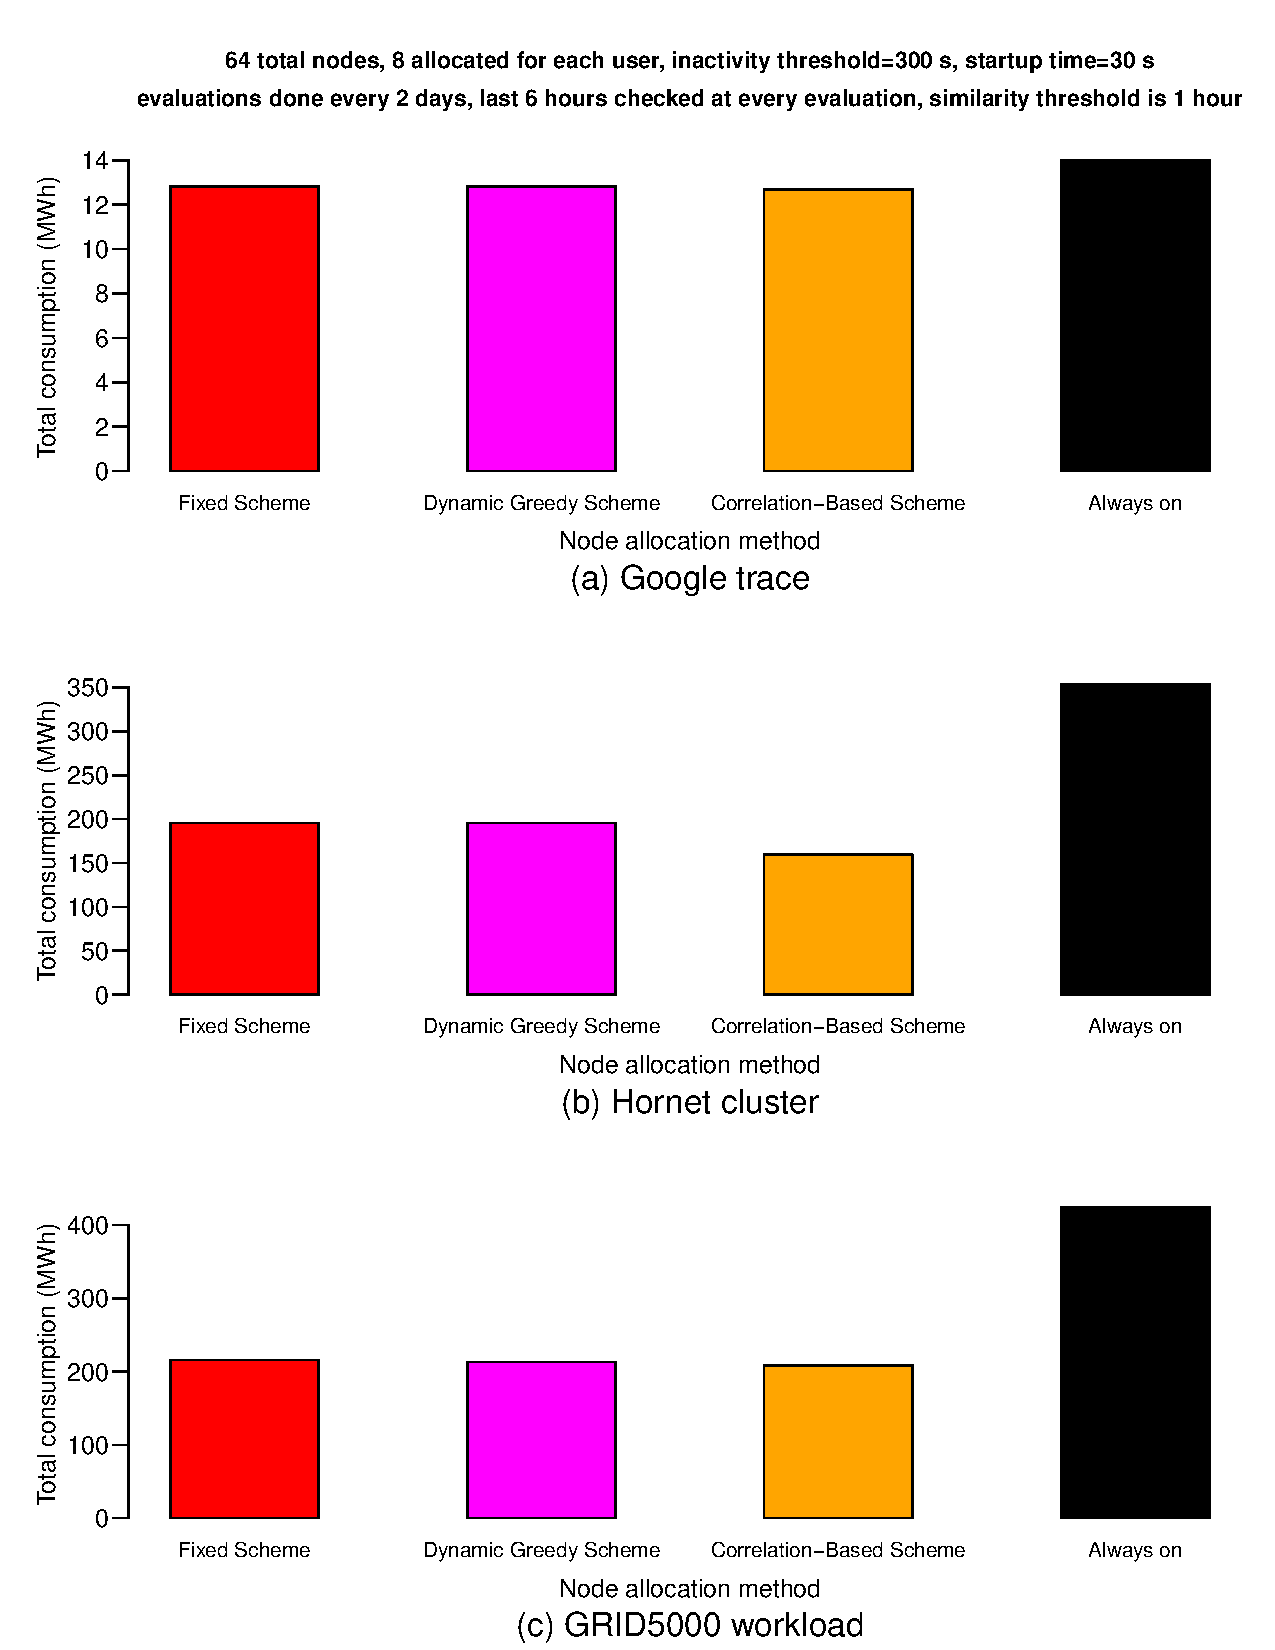
\includegraphics[width=\columnwidth,keepaspectratio]{FIG5.pdf}
\caption{Energy consumption comparison of methods}
\label{bigresult}
\end{figure}

Figure~\ref{bigresult} shows that, for the Google trace any of the methods would deliver the same amount
of energy savings and the percentage of energy savings is 8.4\% at its maximum. Google trace is a highly
I/O intensive workload and there are not many idle periods in the system. As a result, energy savings are
not significant. For Hornet cluster data and GRID5000 workload, we observe that all three workloads save
significant amount of energy. For both of these workloads, we see that Dynamic Greedy scheme does not
improve on energy consumption that much compared to the Fixed scheme. One of the main objectives of the
Dynamic Greedy scheme is to balance load across the storage system. As a result, balancing the load
across the system prevents further energy savings. Correlation-Based scheme provides slightly better energy
savings for GRID5000 workload and much better energy savings for Hornet cluster data. Hornet cluster is mostly
used by researchers working simultaneously on a project which potentially improves the correlation
between storage system users. For Hornet cluster data the energy savings are as high as 55\% and
for GRID5000 workload energy savings are as high as 50.9\%.

\subsection{Fixed Scheme}
We first evaluate the Fixed scheme, where one of the node allocation techniques (balancing, sequential,
random or groups) is chosen and kept active unless manually changed. We calculate the total
energy consumption, load balance and latency per access with 64 total nodes in the system,
where 8 nodes are allocated for each user. Figure~\ref{firstresult} shows how energy consumption, load balance
and latency per access change with each node allocation technique. \textit{Random} node allocation technique is
executed five times and the average result is reported, as it can yield to a different result
at each run. Due to space considerations, we show only the Google trace evaluations of the Fixed scheme,
as other workloads have similar results. 
 
\begin{figure}[!htbp]
\centering
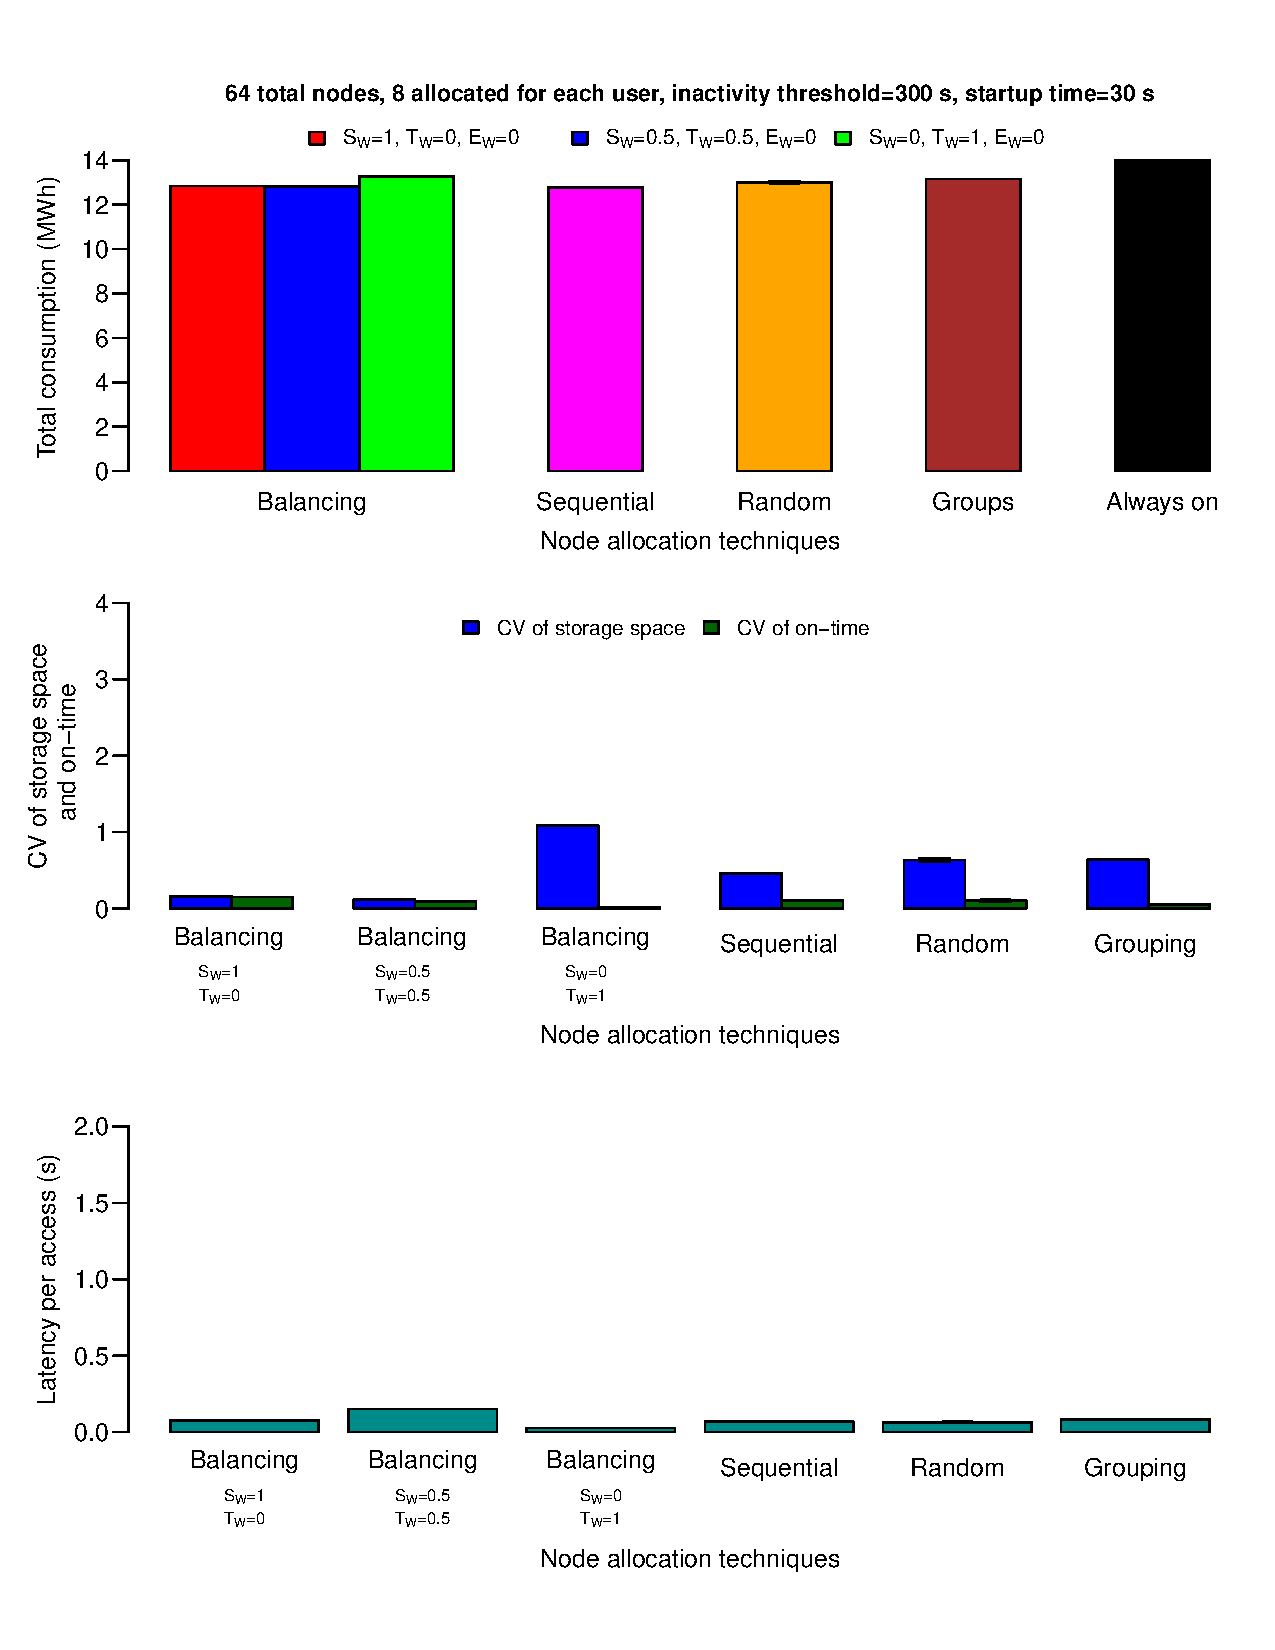
\includegraphics[width=\columnwidth,keepaspectratio]{FIG6.pdf}
\caption{Allocation technique vs energy consumption, load balance and latency per access (Fixed scheme - Google trace)}
\label{firstresult}
\end{figure}

As seen in Figure~\ref{firstresult}, each node allocation technique saves some amount of energy
compared to the stock case where there is no energy saving technique in place (system always on).
The percentage of savings is around 8.4\% for the Google trace. Google trace is highly intensive and as a
result, there are not that many idle periods in this workload. Therefore, energy savings are limited in
such a busy workload.
The amount of energy savings does not
vary much with different techniques. Balancing technique with on-time balancing weight ($T_W$) set to
one consumes slightly more energy compared to other techniques. The primary objective of balancing technique
with on-time balancing weight set to one is to balance the on-time of nodes across the storage system. We found
from the Google trace that majority of the storage system accesses are in the range of couple hundred seconds.
Google trace workload is already balanced initially in terms of node on-time; therefore, balancing technique
with on-time balancing weight set to one does not change the node allocations as much as other techniques do,
resulting in higher energy consumption.

However, the techniques do differ considerably in terms of balancing storage space and on-time. Second sub-plot in
Figure~\ref{firstresult} shows how the coefficient of variation (CV) of storage space and on-time across the storage nodes
vary with different node allocation techniques. As shown in the second sub-plot of Figure~\ref{firstresult}, the
balancing technique with non-zero storage space balancing weight ($S_W$) has smaller CV
of storage space across the storage nodes. Other techniques do not perform that well as their primary objective
is not to balance storage space across the storage nodes.

The balancing technique also performs well for balancing on-time of the storage nodes, as shown in the second sub-plot
of Figure~\ref{firstresult}. Balancing technique with time balancing weight ($T_W$) set to one has the smallest CV
of on-time across the storage nodes as expected.

The third sub-plot in Figure~\ref{firstresult} shows how the latency per access changes with each node allocation technique.
As we have mentioned previously, balancing technique with on-time balancing weight set to one does not change the node
allocations as much as other techniques do. As a result, that technique has the smallest latency per access. On the
other hand, balancing technique with both storage and on-time balancing weight set to 0.5 has the highest energy savings
compared to other techniques; increasing its latency per access. In general, we can see that all techniques have very
close latency per access values, usually around 0.1 seconds. 

\begin{figure}[!htbp]
\centering
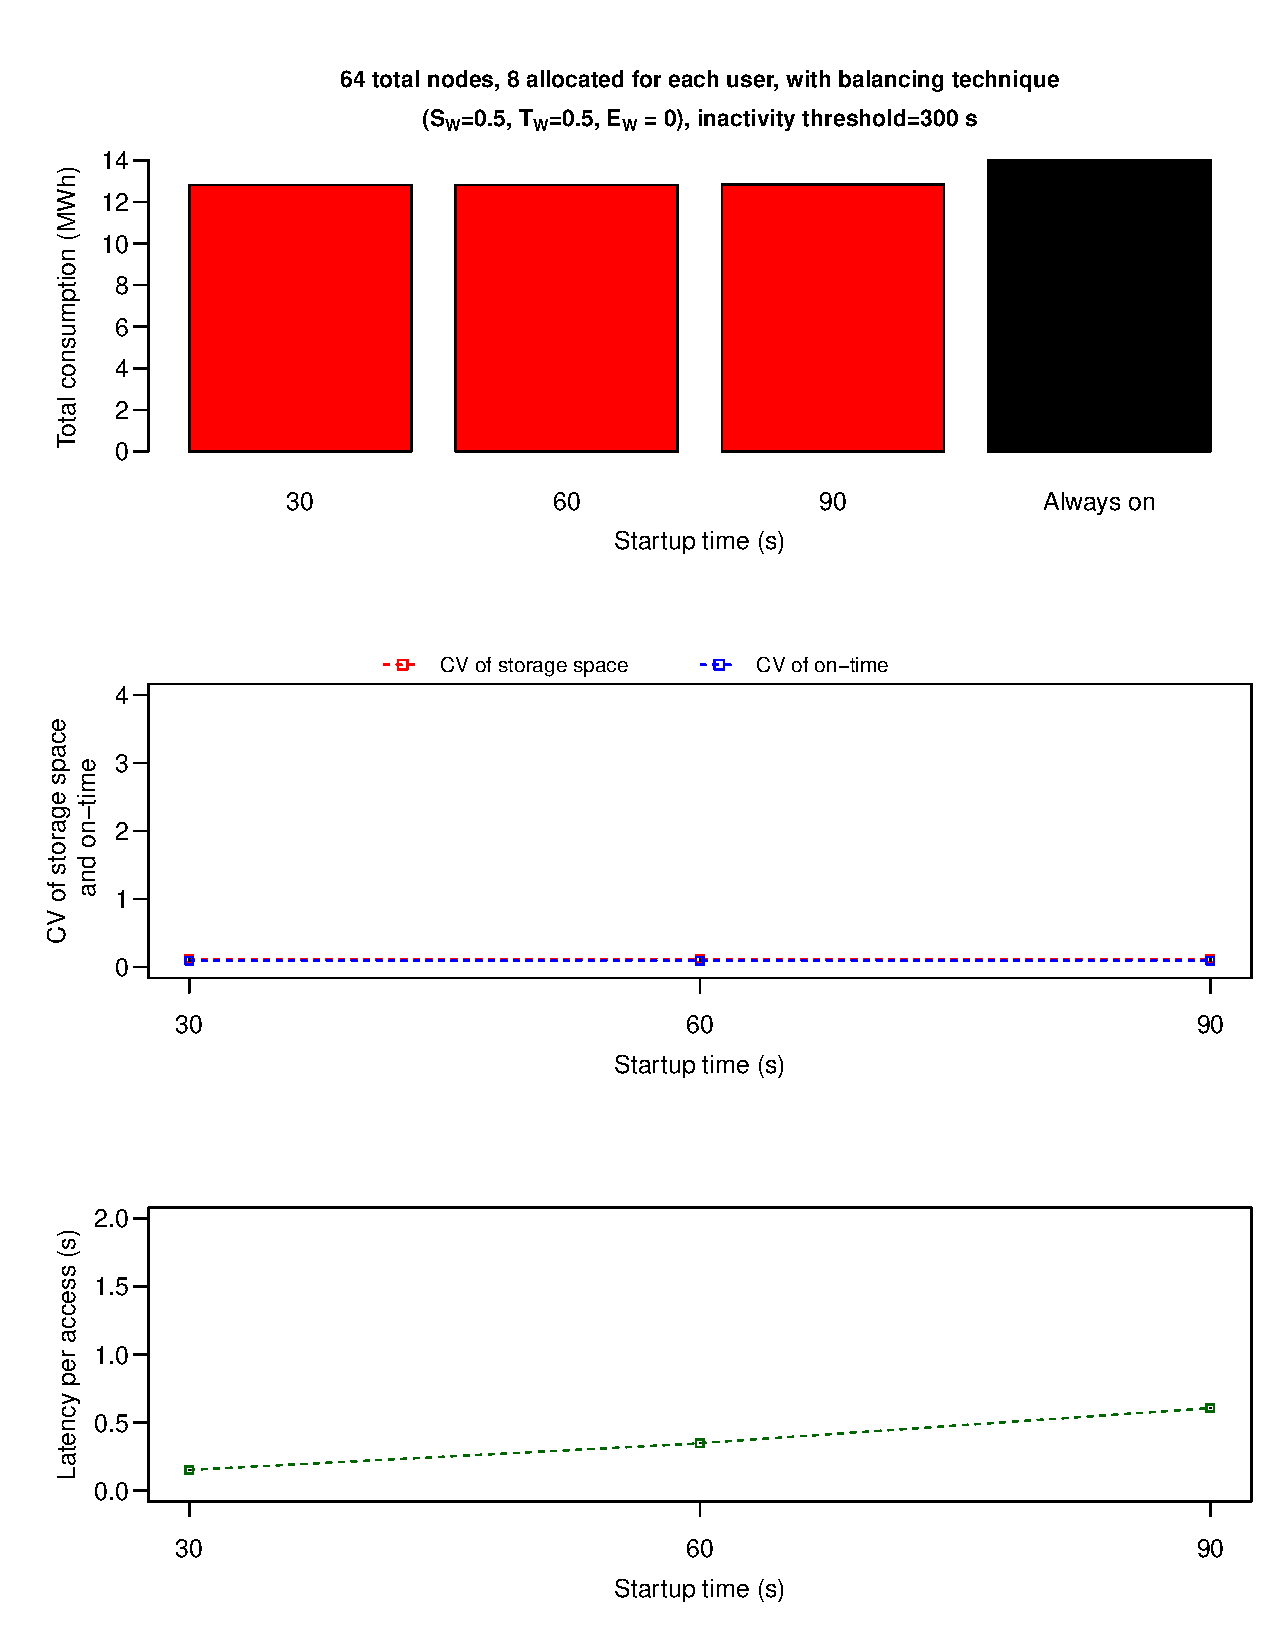
\includegraphics[width=\columnwidth,keepaspectratio]{FIG7.pdf}
\caption{The effect of varying the startup time (Fixed scheme - Google trace)}
\label{secondresult}
\end{figure}

\begin{figure}[!htbp]
\centering
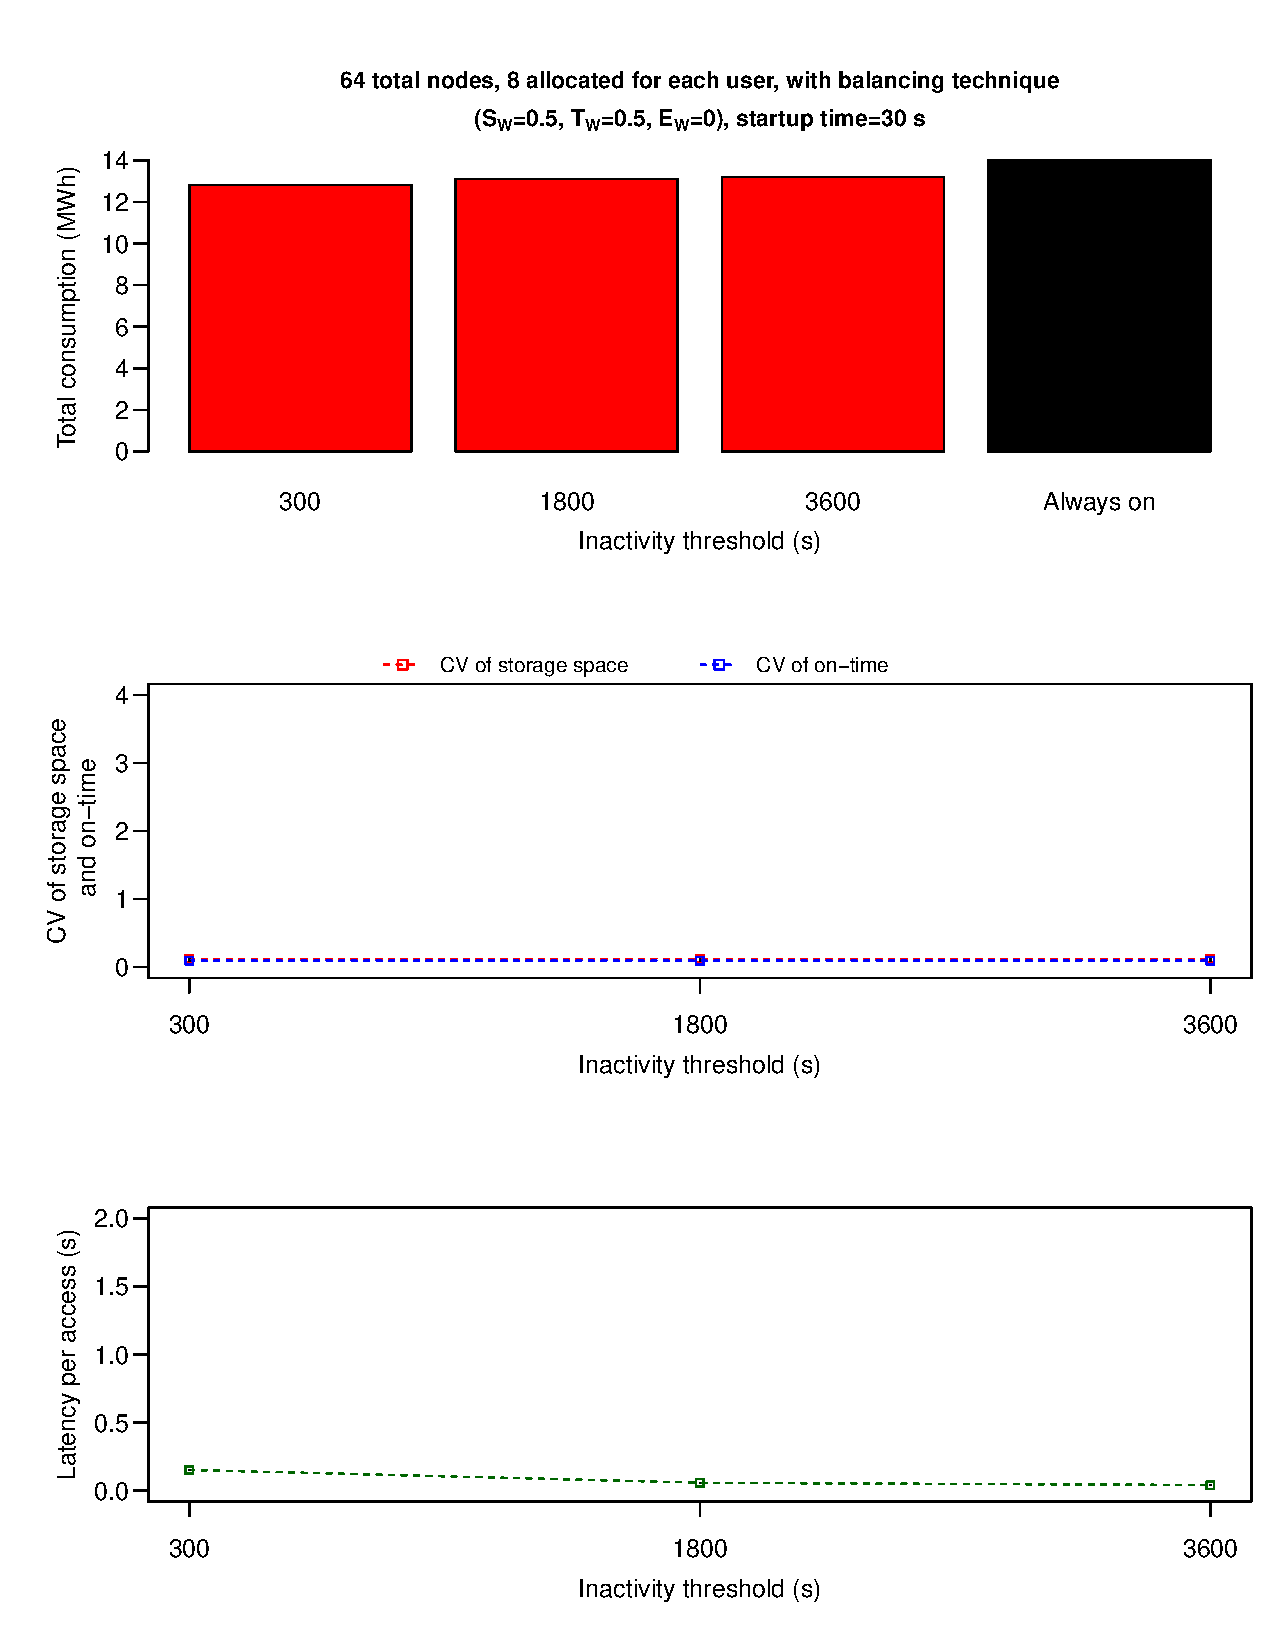
\includegraphics[width=\columnwidth,keepaspectratio]{FIG8.pdf}
\caption{The effect of varying the inactivity threshold (Fixed scheme - Google trace)}
\label{thirdresult}
\end{figure}

We also investigate how the total energy consumption, load balance and latency per access is affected by the changes in
the startup time and inactivity threshold. Figure~\ref{secondresult} shows the total energy consumption,
load balance and latency per access measurements while the startup time is varied between 30, 60 and 90 seconds. Similarly,
Figure~\ref{thirdresult} shows the total energy consumption, load balance and latency per access measurements while the
inactivity threshold is varied between 300, 1800 and 3600 seconds. As each technique is affected similarly by the changes
in the inactivity threshold and startup time, we only present results for the balancing technique with both storage space
and on-time balancing weights ($S_W$ and $T_W$) equal to 0.5 and energy consumption weight ($E_W$) equal to zero.

As we can see in both Figure~\ref{secondresult} and Figure~\ref{thirdresult}, changing the inactivity threshold or the
startup time has nearly no effect on the load balance. Changing the startup time does not affect the energy consumption
either. Figure~\ref{thirdresult} shows that increasing the inactivity threshold causes energy consumption to go up. When
the inactivity threshold is higher, it is less likely for a storage node to be turned-off for being idle longer
than this threshold. This causes the storage node to stay on for longer and consequently increases energy consumption.
Latency per access slightly increases as the startup time is increased. This is expected, since any access that is made
to a turned-off node will wait longer for that node to startup again. On the other hand, as the inactivity threshold is
increased, latency per access slightly decreases. In that case, the storage nodes are kept on for longer due to higher
inactivity threshold; which means that less storage system accesses will be made to a turned-off node.

\subsection{Dynamic Greedy Scheme}
In this section, we evaluate the Dynamic Greedy scheme and find out how effective it is in terms of energy consumption, 
load balance and latency per access. As discussed in Section~\ref{greedy}, \textit{evaluation points} and
\textit{control periods} are two important parameters of the Dynamic Greedy scheme. Dynamic Greedy scheme starts with
one of the four node allocation techniques we proposed (balancing, sequential, random or grouping) and changes between
these techniques at evaluation points, if necessary. We try to understand if the initial technique chosen has any effect
on the energy consumption, load balance or latency. We also analyze the effect of varying evaluation points and
control periods on the energy consumption, load balance and latency per access.

To start with, we test the Dynamic Greedy scheme with varying storage-space, on-time and energy consumption weights
($S_W$, $T_W$ and $E_W$) where the total number of storage nodes in the system is 64 and the number of nodes allocated
for each user is 8, as shown in Figure~\ref{fourthresult}. The evaluations are done every 2 days and the storage
accesses in the last 6 hours are checked. Each measurement is the average of five runs. Due to space considerations, we
show only the Hornet cluster evaluations of the Dynamic Greedy scheme, as other workloads have similar results.

\begin{figure}[!htbp]
\centering
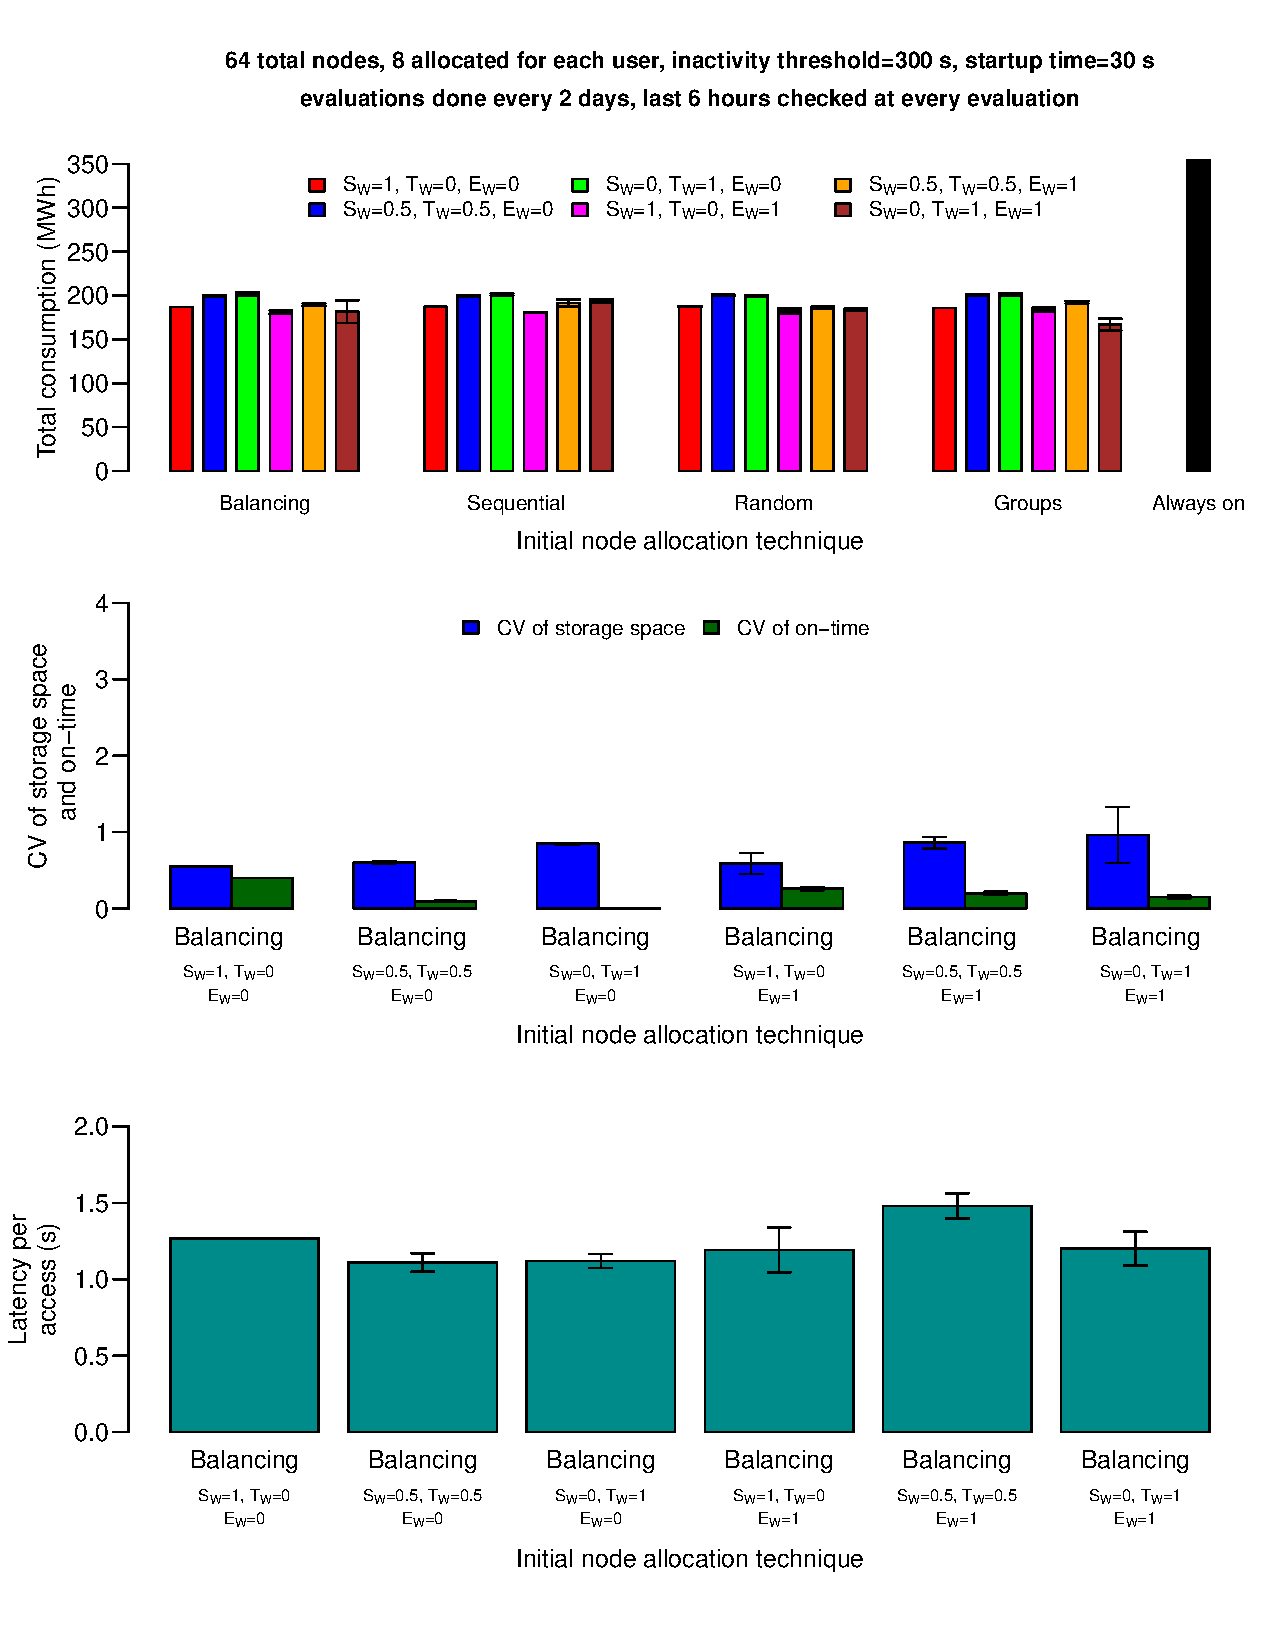
\includegraphics[width=\columnwidth,keepaspectratio]{FIG9.pdf}
\caption{Initial technique vs energy consumption, load balance and latency per access (Dynamic Greedy scheme - Hornet cluster)}
\label{fourthresult}
\end{figure}

Figure~\ref{fourthresult} shows that the Dynamic Greedy scheme saves a considerable amount of energy regardless of
which node allocation technique is chosen initially. The percentage of energy savings are between 43.4\% and 52\%
for varying storage space, on-time and energy weights. Regardless of which technique is initially chosen, we can
see that cases where the energy consumption weight ($E_W$) is set to one consume less energy compared to the cases
where the energy consumption weight is set to zero. Another observation we can make is that the cases where the
on-time balancing weight ($T_W$) is non-zero and energy consumption weight ($E_W$) is set to zero consume more
energy. In the Hornet cluster workload, storage system access lengths vary significantly. As a result,
while trying to balance the on-time across the storage nodes, it is more likely to transfer users from one node
to another. Storage space usage among the users vary as well, though not as much as the access lengths.

In the second sub-plot of Figure~\ref{fourthresult}, we can see how the CVs of storage space and
on-time change when the storage space, on-time and energy consumption weights are varied. Regardless of
which allocation technique is chosen initially (balancing, sequential, random or grouping) the CVs of the
storage space and on-time are similar. Therefore, we only show the results for cases where balancing technique
is the initially chosen technique. We can see that the CV of the storage space is the smallest when the storage space
balancing weight ($S_W$) is set to one, regardless of the energy consumption weight ($E_W$). As the on-time
balancing weight ($T_W$) is increased, the CV of the storage space increases as well. The same holds true
for the CV of the on-time. When the on-time balancing weight ($T_W$) is set to one, the CV of the on-time
is the smallest regardless of the energy consumption weight ($E_W$). As the storage space balancing
weight ($S_W$) is increased, the CV of the on-time increases as well.

We can see how latency per storage access changes with varying storage space, on-time and energy consumption
weights in the third sub-plot of Figure~\ref{fourthresult}. Again, as it does not matter which allocation technique
is initially chosen, we only show the results for cases where the balancing technique is the initially chosen
technique. The latency
measurements are almost the inverse of the energy consumption measurements in the first sub-plot of
Figure~\ref{fourthresult}. In the first sub-plot of Figure~\ref{fourthresult}, we have seen that when the energy
consumption weight ($E_W$) is set to one, the energy consumption goes down. This means that a storage access
will most likely be made on a turned-off node, increasing latency per access. We have also seen in the
first sub-plot of Figure~\ref{fourthresult} that when on-time balancing weight is non-zero and the energy
consumption weight ($E_W$) is set to zero, the energy savings are less. This will in turn
decrease the chance of an access to be made to a turned-off node, decreasing latency per access.

\begin{figure}[!htbp]
\centering
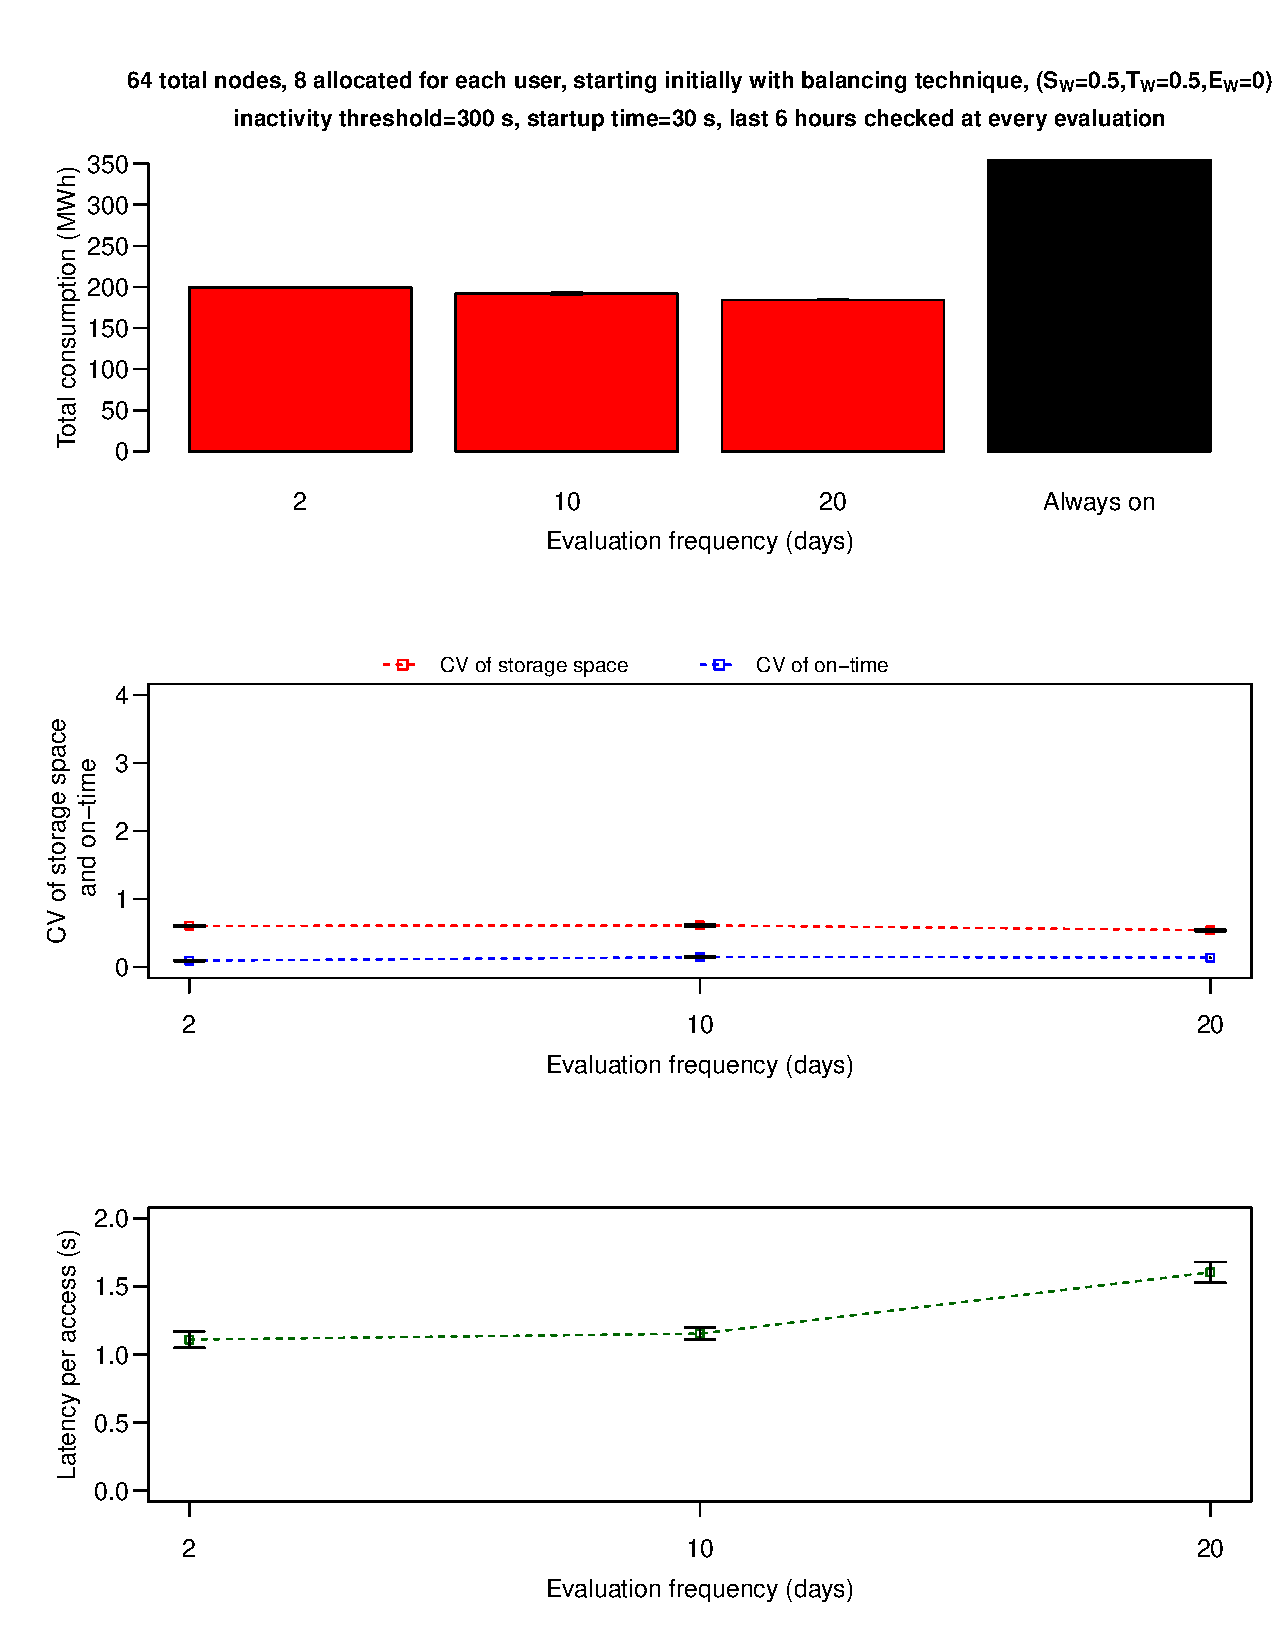
\includegraphics[width=\columnwidth,keepaspectratio]{FIG10.pdf}
\caption{The effect of varying the evaluation frequency (Dynamic Greedy scheme - Hornet cluster)}
\label{fifthresult}
\end{figure}

We now look at the effect of varying the evaluation frequency on the total energy consumption,
load balance and latency per access. The evaluation frequency is varied between 2, 10 and 20 days
and the control period is fixed at 6 hours. Since the initial allocation technique does not change
the results, we initially start with the balancing technique with both storage space and on-time
balancing weights ($S_W$ and $T_W$) set to 0.5 and energy consumption weight ($E_W$) set to zero.
As shown in Figure~\ref{fifthresult}, total energy consumption goes down as the evaluation frequency
becomes longer. When the evaluation frequency is longer, our algorithms have more knowledge about
the state of the storage system. Therefore, more intelligent decisions are made for reducing energy
consumption. We also see that the CVs of the storage space and on-time is almost not affected by
the evaluation frequency. In the third sub-plot of Figure~\ref{fifthresult}, we observe that latency
per access increases as the evaluation frequency becomes longer. This is expected, as longer evaluation
frequency reduces energy consumption by turning off storage nodes more often. 

\begin{figure}[!htbp]
\centering
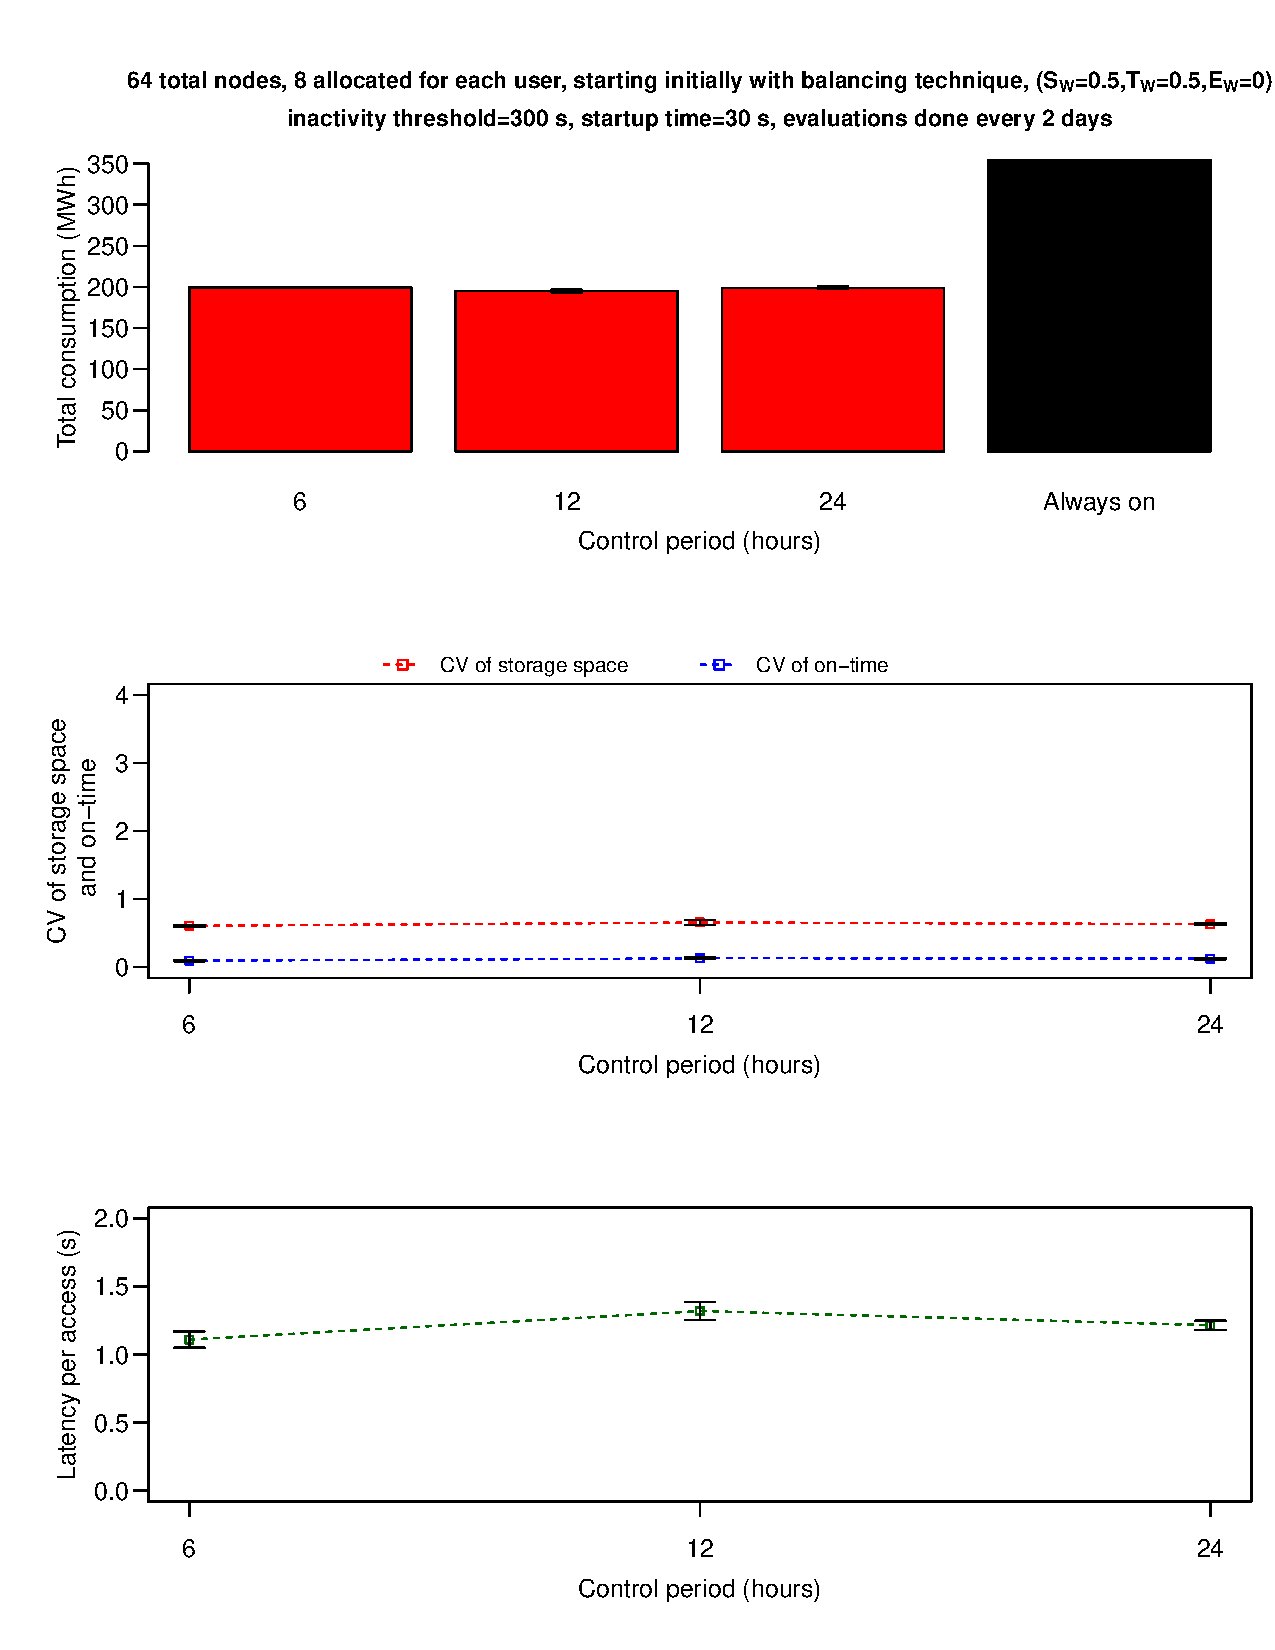
\includegraphics[width=\columnwidth,keepaspectratio]{FIG11.pdf}
\caption{The effect of varying the control period (Dynamic Greedy scheme - Hornet cluster)}
\label{sixthresult}
\end{figure}

Figure~\ref{sixthresult} shows the effect of varying the control period (between 6, 12 and 24 hours)
on the total energy consumption, load balance and latency per access. In this test case the evaluation
frequency is fixed at 2 days. The results in Figure~\ref{sixthresult} indicate that varying the control
period does not affect the total energy consumption, load balance or latency per access.

\subsection{Correlation-Based Scheme}
In this section, we evaluate the Correlation-Based scheme and find out how effective it is in terms of energy consumption,
load balance and latency per access. Correlation-Based scheme starts with one of the four node allocation
techniques (balancing, sequential, random or grouping) similar to the Dynamic Greedy scheme. Unlike the Dynamic
Greedy scheme, it checks the correlations between users at evaluation points and allocates the same storage
nodes for correlated users instead of changing the initial node allocation technique. As a matter of fact,
initial node allocation technique is used if only a user accesses the storage system for the first time.
During the following tests, we also try to understand if the initial technique chosen has any effect on the
energy consumption, load balance or latency per access.

Correlation-Based scheme also has \textit{evaluation point} and \textit{control period} parameters. We have
already shown the effect of varying these two parameters for the Dynamic Greedy scheme; therefore, we are not
repeating the same tests for Correlation-Based scheme. \textit{Similarity threshold} is a parameter that
is unique to the Correlation-Based scheme. We look at the effect of this parameter on the energy consumption,
load balance and latency per access as well.

To start with, we test the Correlation-Based scheme with different initial techniques, where the total number of
storage nodes in the system is 64 and the number of nodes allocated for each user is 8, as shown in 
Figure~\ref{seventhresult}. The evaluations are done every 2 days and the storage accesses in the last 6 hours
are checked. Each measurement is the average of five runs. Since energy consumption weight is not important
in Correlation-Based scheme, it is fixed at zero in this test case. Due to space considerations, we
show only the GRID5000 workload evaluations of the Correlation-Based scheme, as other workloads have similar
results.

\begin{figure}[!htbp]
\centering
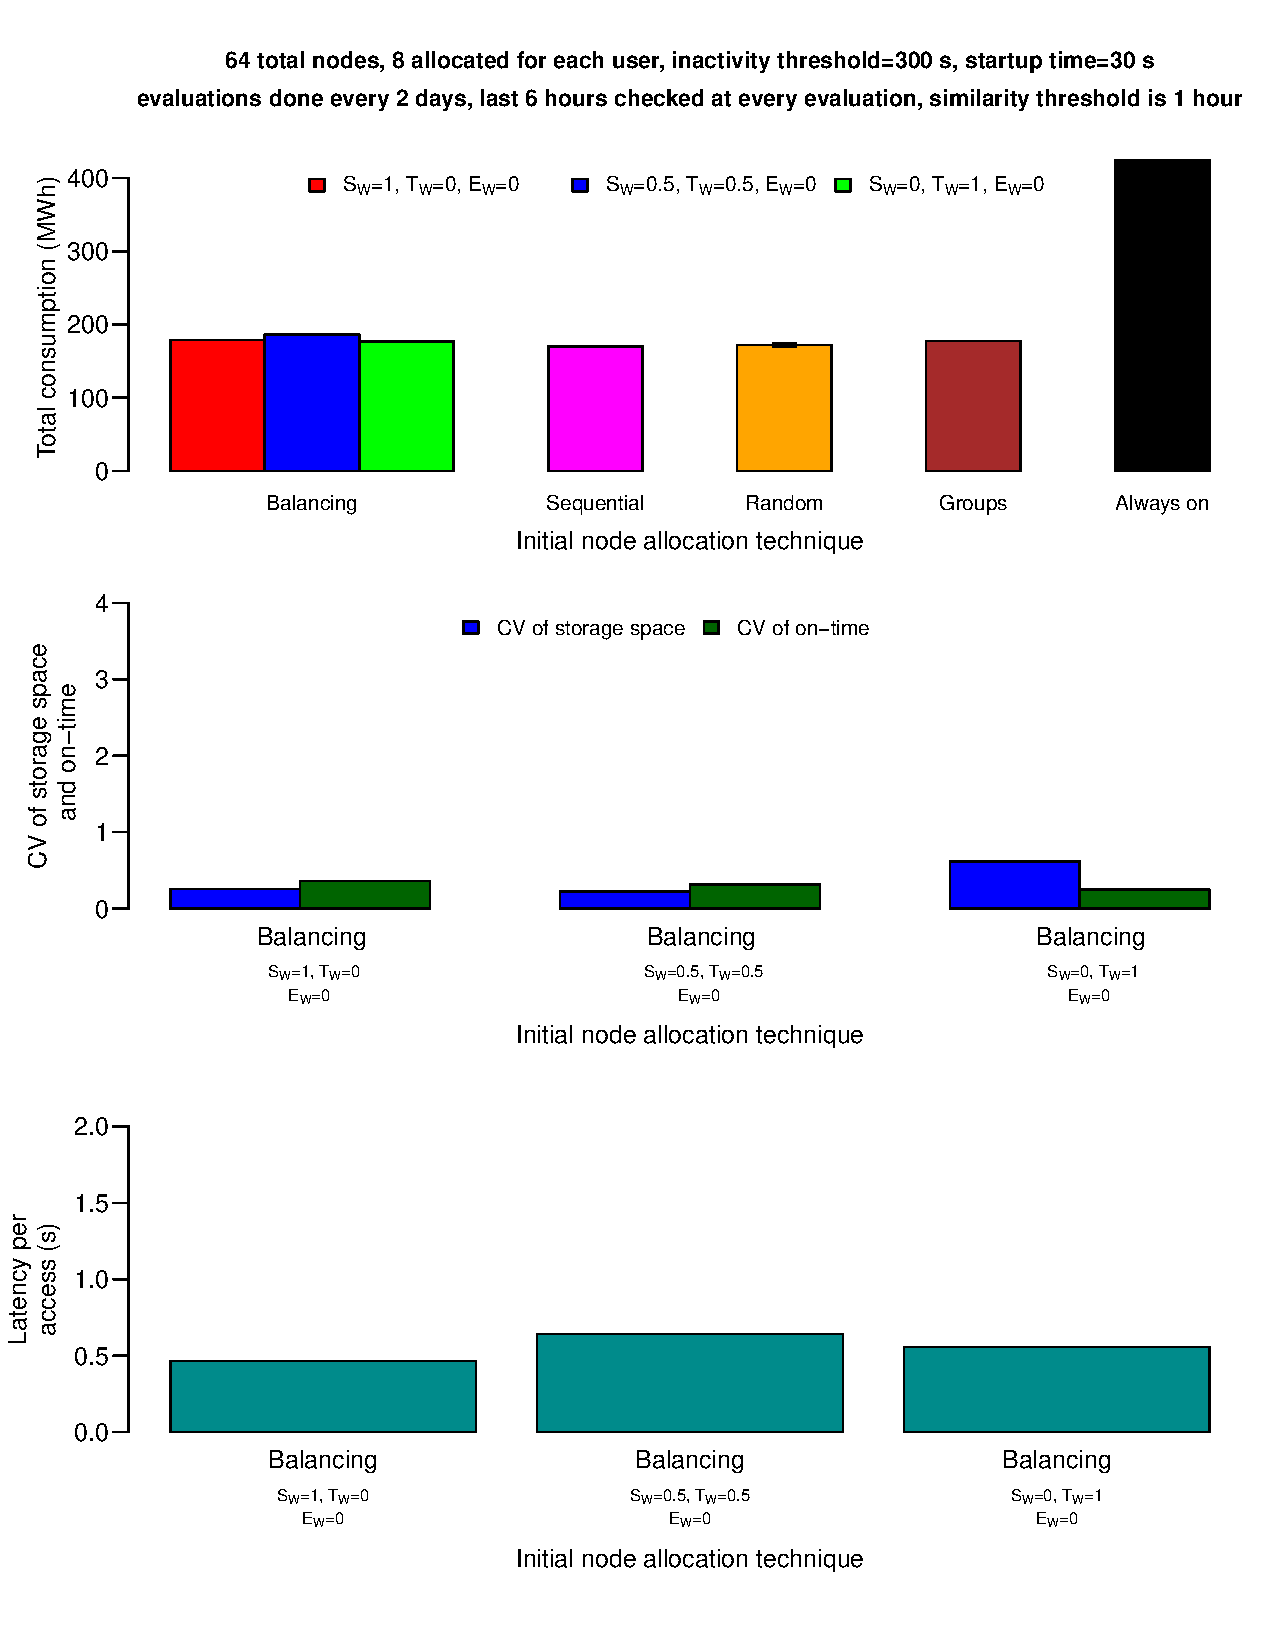
\includegraphics[width=\columnwidth,keepaspectratio]{FIG12.pdf}
\caption{Initial technique vs energy consumption, load balance and latency (Correlation-Based scheme -
 GRID5000 workload)}
\label{seventhresult}
\end{figure}

Figure~\ref{seventhresult} shows that Correlation-Based Scheme saves more than half of the energy consumed
in the stock case regardless of the initial node allocation technique. The percentage of energy savings
are as high as 60\%. We observe that the initial technique chosen does not have a significant effect on
the energy consumption.

The CVs of the storage space and on-time are shown in the second sub-plot of Figure~\ref{seventhresult}.
As the initial technique chosen for the Correlation-Based scheme does not really matter, we show
results for the balancing technique with varying storage-space and on-time balancing weights. As the
storage space balancing weight ($S_W$) is increased, the CV of the storage space
decreases. The same is true for on-time.

The third sub-plot in Figure~\ref{seventhresult} shows how latency per access is affected when the initial
technique is balancing with varying storage-space and on-time balancing weights. In GRID5000 workload, the
storage space usage of users are close to each other. Therefore balancing technique with storage-space
balancing weight set to one will not effect the node allocations as much as other techniques do. We observed
that GRID5000 workload havs accesses of varying lengths, particularly
until the first evaluation point. As a result, if both the storage space balancing and on-time weight are set
to 0.5, then the algorithm will not try to break already balanced storage-space distribution, while at the
same time trying to balance on-time. This will in turn result in more transfers and consequently more latency.
This feature of the GRID5000 workload is similar to that of Google trace in Figure~\ref{firstresult}, except
that Google trace had varying storage space usage among the users where access lenghts did not vary that much.

\begin{figure}[!htbp]
\centering
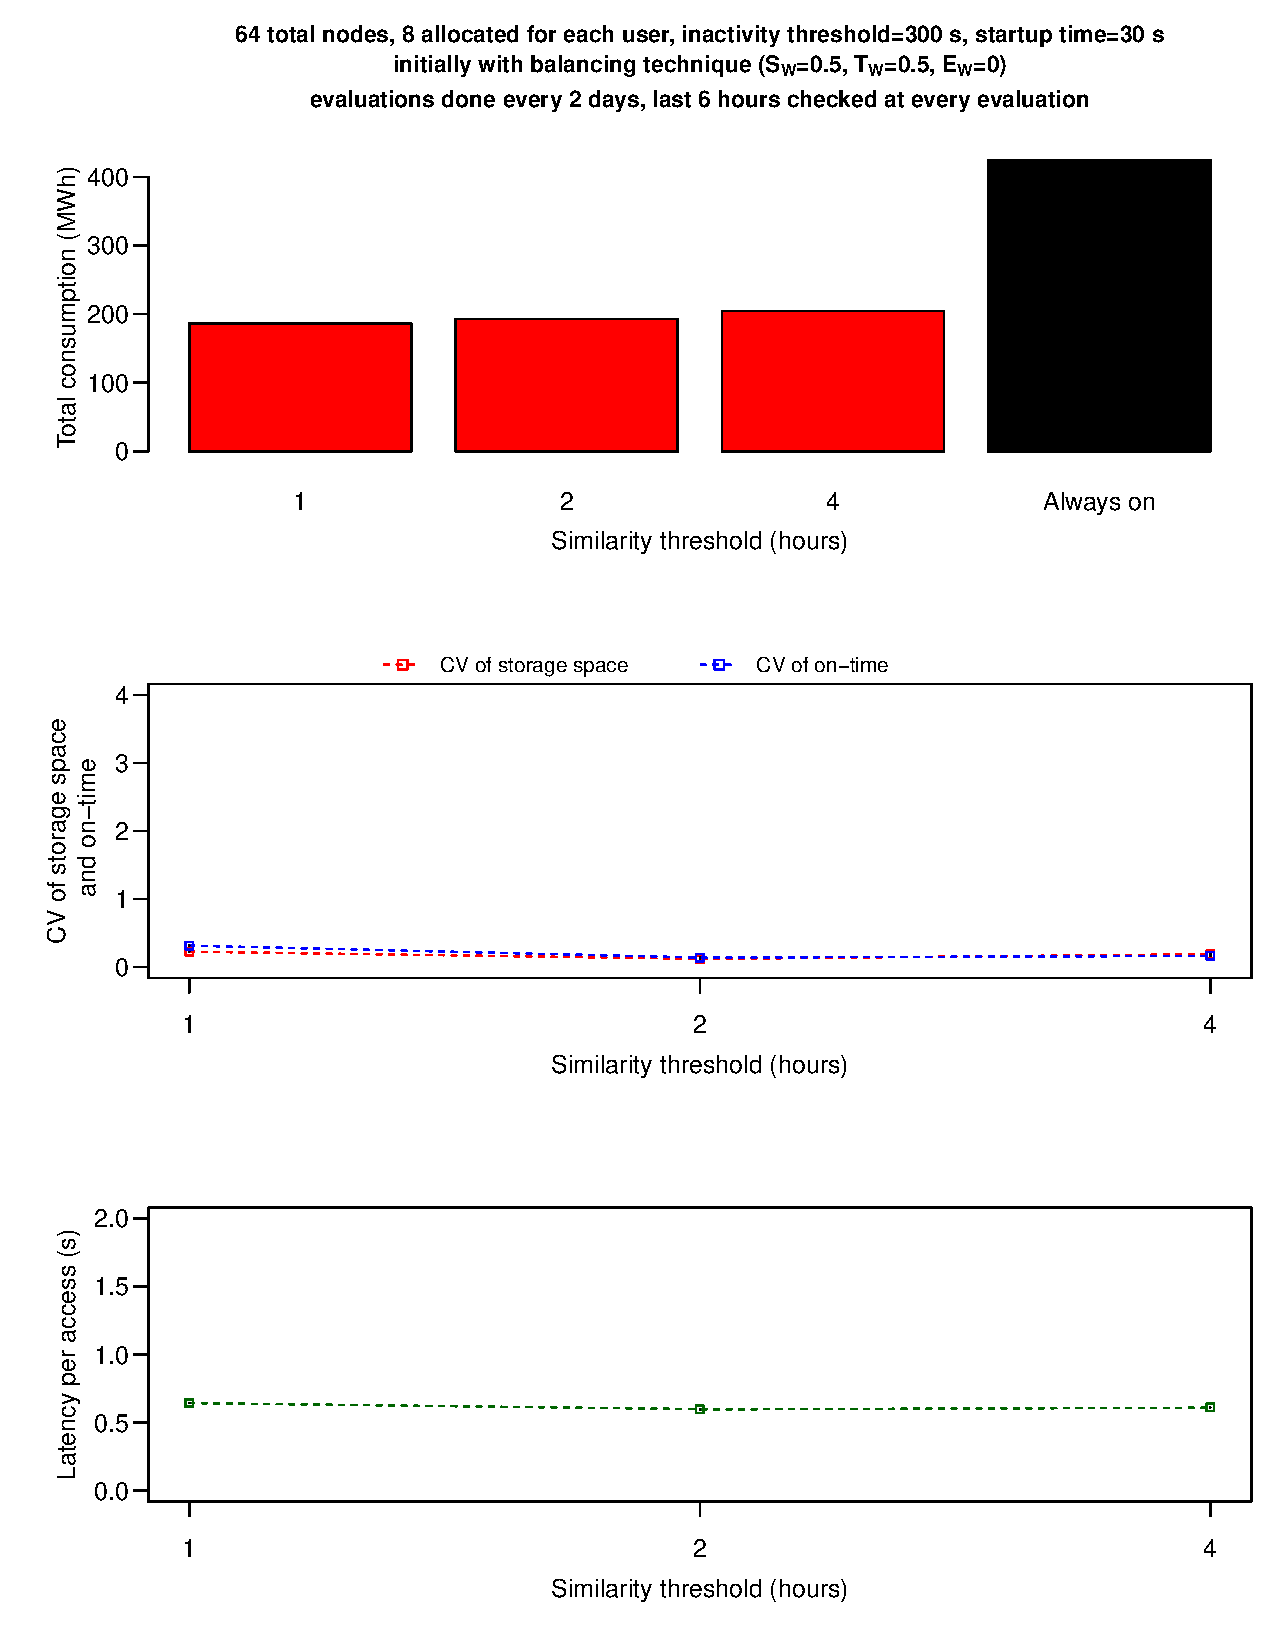
\includegraphics[width=\columnwidth,keepaspectratio]{FIG13.pdf}
\caption{The effect of varying the similarity threshold (Correlation-Based scheme - GRID5000 workload)}
\label{eightthresult}
\end{figure} 

Figure~\ref{eightthresult} shows the effect of varying the similarity threshold on the total energy
consumption, load balancing and latency per access. Evaluations are done every 2 days and the last 6 hours
are checked at every evaluation. Balancing technique with both storage space and on-time balancing
weights set to 0.5 is used initially. Similar to the inactivity threshold, varying the
similarity threshold has almost no effect on the standard devations of the storage space and on-time
or latency per access. When the similarity threshold is increased, total energy consumption
increases slightly. The higher the similarity threshold is, the less likely it is to find correlated
users. As a result, energy consumption goes up with higher similarity threshold.

\subsection{Validating Mathematical Model}
\label{validate_model}
We have validated the mathematical model presented in Section~\ref{model} against the
experimental results of our approach using data from Hornet HPC system. We can estimate the energy
consumption, load balancing and latency per access values for each workload
by using the mathematical model presented in Section~\ref{model}. We validate
the mathematical model using the subset of test parameters as shown in
Table~\ref{tbl:validate_params}.
For brevity, we show only the Hornet data, though the other workloads show similar results.
For the Hornet data that we show here for this validation, we have primarily used a Generalized
Extreme Value interjob arrival model - i.e.
$F(t) = e^{-g(t)},\ \ where\ \ g(t)\ \ =\ \ [{1 + (\frac{t - \mu}{\sigma}) * \xi}]^{\frac{-1}{\xi}}$
and $\xi,\ \ \mu$ and $\sigma$ are distribution parameters.

\begin{table}[!htbp]
 \begin{center}
  \begin{tabular}{|l|l|} \hline
Test Parameter & Values \\ \hline
Total number of nodes          & 64 \\ \hline
Number of nodes allocated        & 8 \\
for each user              & \\ \hline
Allocation methods           & Fixed, Dynamic Greedy, Correlation-Based \\ \hline
Low-energy mode             & Turn Off \\ \hline
Inactivity threshold          & 300 s \\ \hline
Startup time              & 30 s \\ \hline
Similarity threshold          & 3600 s \\ \hline
Storage space and on-time        & 0.5, 0.5, 0 \\
balancing weights            & \\ \hline
Power consumption per node       & 300 W \\ \hline
Workloads                        & Hornet \\ \hline
  \end{tabular}
 \end{center}
 \caption{Mathematical Model Validation Parameters}
 \label{tbl:validate_params}
\end{table}

Tables~\ref{tbl:validate_results_fixed},~\ref{tbl:validate_results_dynamic} and ~\ref{tbl:validate_results_corr} show
that the mathematical model we presented is able to estimate the test result parameters (CV of storage space, CV of on-time
, energy cost and latency per access) accurately in most
cases. The storage space usage of a user per storage node does not change over time; therefore, the chance of
estimating it accurately is high. Our model estimates on-time value and energy consumption of each storage node accurately
as well, as estimating them involves all of the parameters captured by our model except storage space usage.
Latency per access is highly dependent on the arrival rate of \textit{interarrivals} and our model does the best attempt to
capture these interarrivals in order to estimate the latency per access.

\begin{table}[!htbp]
 \begin{center}
 \resizebox{\textwidth}{!}{%
  \begin{tabular}{lcccccccc} \hline
\multicolumn{1}{|c}{} & \multicolumn{4}{c|}{Balancing} & \multicolumn{4}{c|}{Sequential}\\ \hline
\multicolumn{1}{|c}{} & \multicolumn{1}{|c}{Storage} & \multicolumn{1}{c}{On-time} & \multicolumn{1}{c}{Energy} & \multicolumn{1}{c|}{Latency per} & \multicolumn{1}{c}{Storage} & \multicolumn{1}{c}{On-time} & \multicolumn{1}{c}{Energy} & \multicolumn{1}{c|}{Latency per} \\
\multicolumn{1}{|c}{} & \multicolumn{1}{|c}{CV} & \multicolumn{1}{c}{CV} & \multicolumn{1}{c}{cost (MWh)} & \multicolumn{1}{c|}{access (s)} & \multicolumn{1}{c}{CV} & \multicolumn{1}{c}{CV} & \multicolumn{1}{c}{cost (MWh)} & \multicolumn{1}{c|}{access (s)} \\ \hline
\multicolumn{1}{|l|}{Simulation} & 0.539 & 0.312 & 195.65 & \multicolumn{1}{c|}{1.0348} & 0.757 & 0.382 & 181.01 & \multicolumn{1}{c|}{1.1833} \\ 
\multicolumn{1}{|l|}{Model} & 0.543 & 0.3145 & 195.62 & \multicolumn{1}{c|}{1.1657} & 0.7628 & 0.3849 & 180.93 & \multicolumn{1}{c|}{1.1669} \\
\multicolumn{1}{|l|}{Error} & 0.74\% & 0.80\% & 0.02\% & \multicolumn{1}{c|}{12.65\%} & 0.77\% & 0.76\% & 0.04\% & \multicolumn{1}{c|}{1.39\%} \\ \hline
& & & & & & & & \\ \hline
\multicolumn{1}{|c}{} & \multicolumn{4}{c|}{Random} & \multicolumn{4}{c|}{Groups}\\ \hline
\multicolumn{1}{|c}{} & \multicolumn{1}{|c}{Storage} & \multicolumn{1}{c}{On-time} & \multicolumn{1}{c}{Energy} & \multicolumn{1}{c|}{Latency per} & \multicolumn{1}{c}{Storage} & \multicolumn{1}{c}{On-time} & \multicolumn{1}{c}{Energy} & \multicolumn{1}{c|}{Latency per} \\
\multicolumn{1}{|c}{} & \multicolumn{1}{|c}{CV} & \multicolumn{1}{c}{CV} & \multicolumn{1}{c}{cost (MWh)} & \multicolumn{1}{c|}{access (s)} & \multicolumn{1}{c}{CV} & \multicolumn{1}{c}{CV} & \multicolumn{1}{c}{cost (MWh)} & \multicolumn{1}{c|}{access (s)} \\ \hline
\multicolumn{1}{|l|}{Simulation} & 0.9 & 0.394 & 179.81 & \multicolumn{1}{c|}{1.5673} & 1.129 & 0.351 & 183.78 & \multicolumn{1}{c|}{1.0367} \\ 
\multicolumn{1}{|l|}{Model} & 0.9069 & 0.3973 & 179.753 & \multicolumn{1}{c|}{1.2496} & 1.1381 & 0.3539 & 183.711 & \multicolumn{1}{c|}{1.0539} \\
\multicolumn{1}{|l|}{Error} & 0.77\% & 0.84\% & 0.03\% & \multicolumn{1}{c|}{20.27\%} & 0.81\% & 0.83\% & 0.04\% & \multicolumn{1}{c|}{1.66\%} \\ \hline
  \end{tabular}}
 \end{center}
 \caption{Mathematical Model Validation Results for Fixed Scheme}
 \label{tbl:validate_results_fixed}
\end{table}

\begin{table}[!htbp]
 \begin{center}
 \resizebox{\textwidth}{!}{%
  \begin{tabular}{lcccccccc} \hline
\multicolumn{1}{|c}{} & \multicolumn{4}{c|}{Starts with Balancing} & \multicolumn{4}{c|}{Starts with Sequential}\\ \hline
\multicolumn{1}{|c}{} & \multicolumn{1}{|c}{Storage} & \multicolumn{1}{c}{On-time} & \multicolumn{1}{c}{Energy} & \multicolumn{1}{c|}{Latency per} & \multicolumn{1}{c}{Storage} & \multicolumn{1}{c}{On-time} & \multicolumn{1}{c}{Energy} & \multicolumn{1}{c|}{Latency per} \\
\multicolumn{1}{|c}{} & \multicolumn{1}{|c}{CV} & \multicolumn{1}{c}{CV} & \multicolumn{1}{c}{cost (MWh)} & \multicolumn{1}{c|}{access (s)} & \multicolumn{1}{c}{CV} & \multicolumn{1}{c}{CV} & \multicolumn{1}{c}{cost (MWh)} & \multicolumn{1}{c|}{access (s)} \\ \hline
\multicolumn{1}{|l|}{Simulation} & 0.605 & 0.0932 & 199.36 & \multicolumn{1}{c|}{1.11008} & 0.6186 & 0.0956 & 199.273 & \multicolumn{1}{c|}{1.12687} \\
\multicolumn{1}{|l|}{Model} & 0.6031 & 0.1006 & 199.913 & \multicolumn{1}{c|}{1.0424} & 0.6142 & 0.1 & 200.254 & \multicolumn{1}{c|}{0.9944} \\
\multicolumn{1}{|l|}{Error} & 0.31\% & 7.94\% & 0.28\% & \multicolumn{1}{c|}{6.1\%} & 0.71\% & 4.6\% & 0.49\% & \multicolumn{1}{c|}{11.76\%} \\ \hline
& & & & & & & & \\ \hline
\multicolumn{1}{|c}{} & \multicolumn{4}{c|}{Starts with Random} & \multicolumn{4}{c|}{Starts with Groups}\\ \hline
\multicolumn{1}{|c}{} & \multicolumn{1}{|c}{Storage} & \multicolumn{1}{c}{On-time} & \multicolumn{1}{c}{Energy} & \multicolumn{1}{c|}{Latency per} & \multicolumn{1}{c}{Storage} & \multicolumn{1}{c}{On-time} & \multicolumn{1}{c}{Energy} & \multicolumn{1}{c|}{Latency per} \\
\multicolumn{1}{|c}{} & \multicolumn{1}{|c}{CV} & \multicolumn{1}{c}{CV} & \multicolumn{1}{c}{cost (MWh)} & \multicolumn{1}{c|}{access (s)} & \multicolumn{1}{c}{CV} & \multicolumn{1}{c}{CV} & \multicolumn{1}{c}{cost (MWh)} & \multicolumn{1}{c|}{access (s)} \\ \hline
\multicolumn{1}{|l|}{Simulation} & 0.614 & 0.0926 & 200.199 & \multicolumn{1}{c|}{1.14529} & 0.63 & 0.086 & 200.558 & \multicolumn{1}{c|}{1.09082} \\
\multicolumn{1}{|l|}{Model} & 0.6092 & 0.0923 & 199.577 & \multicolumn{1}{c|}{1.022} & 0.6382 & 0.08 & 201.176 & \multicolumn{1}{c|}{1.0311} \\
\multicolumn{1}{|l|}{Error} & 0.78\% & 0.32\% & 0.31\% & \multicolumn{1}{c|}{10.76\%} & 1.3\% & 6.98\% & 0.31\% & \multicolumn{1}{c|}{5.47\%} \\ \hline
  \end{tabular}}
 \end{center}
 \caption{Mathematical Model Validation Results for Dynamic Greedy Scheme}
 \label{tbl:validate_results_dynamic}
\end{table}

\begin{table}[!htbp]
 \begin{center}
 \resizebox{\textwidth}{!}{%
  \begin{tabular}{lcccccccc} \hline
\multicolumn{1}{|c}{} & \multicolumn{4}{c|}{Starts with Balancing} & \multicolumn{4}{c|}{Starts with Sequential}\\ \hline
\multicolumn{1}{|c}{} & \multicolumn{1}{|c}{Storage} & \multicolumn{1}{c}{On-time} & \multicolumn{1}{c}{Energy} & \multicolumn{1}{c|}{Latency per} & \multicolumn{1}{c}{Storage} & \multicolumn{1}{c}{On-time} & \multicolumn{1}{c}{Energy} & \multicolumn{1}{c|}{Latency per} \\
\multicolumn{1}{|c}{} & \multicolumn{1}{|c}{CV} & \multicolumn{1}{c}{CV} & \multicolumn{1}{c}{cost (MWh)} & \multicolumn{1}{c|}{access (s)} & \multicolumn{1}{c}{CV} & \multicolumn{1}{c}{CV} & \multicolumn{1}{c}{cost (MWh)} & \multicolumn{1}{c|}{access (s)} \\ \hline
\multicolumn{1}{|l|}{Simulation} & 2.059 & 0.35 & 120.842 & \multicolumn{1}{c|}{1.27998} & 2.108 & 0.671 & 105.857 & \multicolumn{1}{c|}{1.27017} \\
\multicolumn{1}{|l|}{Model} & 2.0755 & 0.3523 & 120.798 & \multicolumn{1}{c|}{1.5492} & 2.1244 & 0.676 & 105.826 & \multicolumn{1}{c|}{1.2532} \\
\multicolumn{1}{|l|}{Error} & 0.80\% & 0.66\% & 0.04\% & \multicolumn{1}{c|}{21.03\%} & 0.78\% & 0.75\% & 0.03\% & \multicolumn{1}{c|}{1.34\%} \\ \hline
& & & & & & & & \\ \hline
\multicolumn{1}{|c}{} & \multicolumn{4}{c|}{Starts with Random} & \multicolumn{4}{c|}{Starts with Groups}\\ \hline
\multicolumn{1}{|c}{} & \multicolumn{1}{|c}{Storage} & \multicolumn{1}{c}{On-time} & \multicolumn{1}{c}{Energy} & \multicolumn{1}{c|}{Latency per} & \multicolumn{1}{c}{Storage} & \multicolumn{1}{c}{On-time} & \multicolumn{1}{c}{Energy} & \multicolumn{1}{c|}{Latency per} \\
\multicolumn{1}{|c}{} & \multicolumn{1}{|c}{CV} & \multicolumn{1}{c}{CV} & \multicolumn{1}{c}{cost (MWh)} & \multicolumn{1}{c|}{access (s)} & \multicolumn{1}{c}{CV} & \multicolumn{1}{c}{CV} & \multicolumn{1}{c}{cost (MWh)} & \multicolumn{1}{c|}{access (s)} \\ \hline
\multicolumn{1}{|l|}{Simulation} & 2.056 & 0.638 & 103.395 & \multicolumn{1}{c|}{1.36857} & 2.052 & 0.835 & 107.887 & \multicolumn{1}{c|}{1.30135} \\
\multicolumn{1}{|l|}{Model} & 2.072 & 0.6427 & 103.381 & \multicolumn{1}{c|}{1.5413} & 2.0678 & 0.842 & 107.851 & \multicolumn{1}{c|}{1.249} \\
\multicolumn{1}{|l|}{Error} & 0.78\% & 0.74\% & 0.01\% & \multicolumn{1}{c|}{12.62\%} & 0.77\% & 0.84\% & 0.03\% & \multicolumn{1}{c|}{4.02\%} \\ \hline
  \end{tabular}}
 \end{center}
 \caption{Mathematical Model Validation Results for Correlation-Based Scheme}
 \label{tbl:validate_results_corr}
\end{table}

\section{Conclusion}
\label{conclusion}
%%In this work, we presented three different energy-aware node allocation
methods that take advantage of storage network incasting and exploit user
metadata for allocating cloud storage system resources for each user, while
adhering to load-balancing parameters on demand. We also presented a mathematical
model to estimate the outcome of the proposed methods and showed that the estimations
of this model closely match with the simulation results. Each method has been
evaluated both theoretically and through simulation-based tests using real-world
workloads. Theoretical analysis results show that our proposed methods
can provide 2-approximation solutions for minimizing energy consumption
and balancing system load (storage space usage or on-time). Simulation-based
tests show that the energy savings are as high as 60\%. The simulation-based 
tests further show that as the storage system moves from the Fixed scheme to
Dynamic Greedy scheme and then to Correlation-Based scheme, energy savings, latency
per access and coefficient of variation of the storage space and on-time increase. Therefore,
these schemes can be implemented in a cloud storage system depending on parameters
of importance (energy consumption, latency or load balancing). As an example, in
a storage system where energy consumption is the primary concern, Correlation-Based
scheme can be used. Similarly, in a storage system where load balancing and energy consumption
are equally important, Dynamic Greedy scheme can be used. We should also point
out that the latency per access values for any of the methods we proposed were
usually less than a second, which should be acceptable for most of the cloud
storage applications.

Our methods are different from related studies as we classify and place users; rather
than classifying and placing data. Additionally,
the methods we propose take load-balancing and data transfer costs into account,
which is not included in many related studies. We also have a lightweight algorithm
to predict future which is another concept that is missing in related studies, as
they mostly try to predict future reactively by monitoring the system with complex
mechanisms and possibly introducing overhead as a result of this.

The methods we presented in this work can be implemented in any type of general
storage system; including archival and parallel HPC storage systems. We evaluated
these methods with theoretical and simulation-based evaluations. A more insightful
evaluation of these methods can be conducted on a real cloud storage system. The
proposed methods were tested with up to 64 storage nodes, where 8 storage nodes at
maximum were allocated per user. Additionally, the workloads we used had at most
645 users. In a real implementation these numbers might be different; therefore,
further evaluation in a real storage system with different workloads would be also
helpful in this respect. Moreover, we assumed that the low-energy mode for a
storage node is turning it off completely. We are aware that modern disks support
various operating modes with different power requirements; therefore, it would be
interesting to evaluate our methods with disks supporting multiple operating modes.
Future research directions also include implementing the proposed methods with various
types of user-metadata other than the ones used in this work (system usage patterns,
user identifiers etc.) and to investigate the effectiveness of the proposed methods
in a storage system with mechanisms already preventing incasting.

In this work, we presented three different energy-aware node allocation
methods that take advantage of storage network incasting and exploit user
metadata for allocating cloud storage system resources for each user, while
adhering to load-balancing parameters on demand. We also presented a mathematical
model to estimate the outcome of the proposed methods and showed that the estimations
of this model closely match with the simulation results. Each method has been
evaluated both theoretically and through simulation-based tests using real-world
workloads. Theoretical analysis results show that our proposed methods
can provide 2-approximation solutions for minimizing energy consumption
and balancing system load (storage space usage or on-time). Simulation-based
tests show that the energy savings are as high as 60\%. The simulation-based 
tests further show that as the storage system moves from the Fixed scheme to
Dynamic Greedy scheme and then to Correlation-Based scheme, energy savings, latency
per access and coefficient of variation of the storage space and on-time increase. Therefore,
these schemes can be implemented in a cloud storage system depending on parameters
of importance (energy consumption, latency or load balancing). As an example, in
a storage system where energy consumption is the primary concern, Correlation-Based
scheme can be used. Similarly, in a storage system where load balancing and energy consumption
are equally important, Dynamic Greedy scheme can be used. We should also point
out that the latency per access values for any of the methods we proposed were
usually less than a second, which should be acceptable for most of the cloud
storage applications.

Our methods are different from related studies as we classify and place users; rather
than classifying and placing data. Additionally,
the methods we propose take load-balancing and data transfer costs into account,
which is not included in many related studies. We also have a lightweight algorithm
to predict future which is another concept that is missing in related studies, as
they mostly try to predict future reactively by monitoring the system with complex
mechanisms and possibly introducing overhead as a result of this.

The methods we presented in this work can be implemented in any type of general
storage system; including archival and parallel HPC storage systems. We evaluated
these methods with theoretical and simulation-based evaluations. A more insightful
evaluation of these methods can be conducted on a real cloud storage system. The
proposed methods were tested with up to 64 storage nodes, where 8 storage nodes at
maximum were allocated per user. Additionally, the workloads we used had at most
645 users. In a real implementation these numbers might be different; therefore,
further evaluation in a real storage system with different workloads would be also
helpful in this respect. Moreover, we assumed that the low-energy mode for a
storage node is turning it off completely. We are aware that modern disks support
various operating modes with different power requirements; therefore, it would be
interesting to evaluate our methods with disks supporting multiple operating modes.
Future research directions also include implementing the proposed methods with various
types of user-metadata other than the ones used in this work (system usage patterns,
user identifiers etc.) and to investigate the effectiveness of the proposed methods
in a storage system with mechanisms already preventing incasting.

\section{Acknowledgement}
\label{ack}
%%This work was supported in part by a NSF High End Computing University
Research Activity grant (award number CCF-0937879). Any opinions,
findings and conclusions or recommendations expressed in this material
are those of the authors and do not necessarily reflect those of the
NSF. The authors would also like to thank the valuable assistance of staff
at the UConn Booth Engineering Center for Advanced Technologies in
providing access to cluster resources which facilitated this research.

This work was supported in part by a NSF High End Computing University
Research Activity grant (award number CCF-0937879). Any opinions,
findings and conclusions or recommendations expressed in this material
are those of the authors and do not necessarily reflect those of the
NSF. The authors would also like to thank the valuable assistance of staff
at the UConn Booth Engineering Center for Advanced Technologies in
providing access to cluster resources which facilitated this research.

%%\section{}
%%\label{}

%% The Appendices part is started with the command \appendix;
%% appendix  are then done as normal 
%% \appendix

%% \section{}
%% \label{}

%% If you have bibdatabase file and want bibtex to generate the
%% bibitems, please use
%%
%%\bibliographystyle{elsarticle-num} 
%%\bibliography{storage,parallel,energy,macros}

%% else use the following coding to input the bibitems directly in the
%% TeX file.

%%\begin{thebibliography}{00}

%% \bibitem{label}
%% Text of bibliographic item

%%\bibitem{}

%%\end{thebibliography}
\begin{thebibliography}{10}
\expandafter\ifx\csname url\endcsname\relax
  \def\url#1{\texttt{#1}}\fi
\expandafter\ifx\csname urlprefix\endcsname\relax\def\urlprefix{URL }\fi
\expandafter\ifx\csname href\endcsname\relax
  \def\href#1#2{#2} \def\path#1{#1}\fi

\bibitem{googlece}
{Google Cloud Platform}, https://cloud.google.com/compute/.

\bibitem{aws}
{Amazon Web Services}, http://aws.amazon.com/.

\bibitem{azure}
{Microsoft Azure Cloud Computing Platform}, http://azure.microsoft.com/.

\bibitem{Kaushik:2010:LSE:1851476.1851523}
R.~T. Kaushik, L.~Cherkasova, R.~Campbell, K.~Nahrstedt,
  \href{http://doi.acm.org/10.1145/1851476.1851523}{Lightning: Self-adaptive,
  energy-conserving, multi-zoned, commodity green cloud storage system}, in:
  Proceedings of the 19th ACM International Symposium on High Performance
  Distributed Computing, HPDC '10, ACM, New York, NY, USA, 2010, pp. 332--335.
\newblock \href {http://dx.doi.org/10.1145/1851476.1851523}
  {\path{doi:10.1145/1851476.1851523}}.
\newline\urlprefix\url{http://doi.acm.org/10.1145/1851476.1851523}

\bibitem{koomey2011growth}
J.~Koomey, Growth in data center electricity use 2005 to 2010.

\bibitem{Harnik:2009:LPM:1586640.1587438}
D.~Harnik, D.~Naor, I.~Segall,
  \href{http://dx.doi.org/10.1109/IPDPS.2009.5161231}{Low power mode in cloud
  storage systems}, in: Proceedings of the 2009 IEEE International Symposium on
  Parallel\&Distributed Processing, IPDPS '09, IEEE Computer Society,
  Washington, DC, USA, 2009, pp. 1--8.
\newblock \href {http://dx.doi.org/10.1109/IPDPS.2009.5161231}
  {\path{doi:10.1109/IPDPS.2009.5161231}}.
\newline\urlprefix\url{http://dx.doi.org/10.1109/IPDPS.2009.5161231}

\bibitem{Kim:2011:EPD:1951365.1951378}
J.~Kim, D.~Rotem, \href{http://doi.acm.org/10.1145/1951365.1951378}{Energy
  proportionality for disk storage using replication}, in: Proceedings of the
  14th International Conference on Extending Database Technology, EDBT/ICDT
  '11, ACM, New York, NY, USA, 2011, pp. 81--92.
\newblock \href {http://dx.doi.org/10.1145/1951365.1951378}
  {\path{doi:10.1145/1951365.1951378}}.
\newline\urlprefix\url{http://doi.acm.org/10.1145/1951365.1951378}

\bibitem{netapp_power}
L.~Freeman, {Reducing Data Center Power Consumption Through Efficient Storage},
  Tech. rep., NetApp, Inc. (2009).

\bibitem{Miller93}
E.~L. Miller, R.~H. Katz, {An Analysis of File Migration in a Unix
  Supercomputing Environment}, in: USENIX---Winter 1993, 1993.

\bibitem{Kaushik:2010:GTE:1924920.1924927}
R.~T. Kaushik, M.~Bhandarkar,
  \href{http://dl.acm.org/citation.cfm?id=1924920.1924927}{Greenhdfs: Towards
  an energy-conserving, storage-efficient, hybrid hadoop compute cluster}, in:
  Proceedings of the 2010 International Conference on Power Aware Computing and
  Systems, HotPower'10, USENIX Association, Berkeley, CA, USA, 2010, pp. 1--9.
\newline\urlprefix\url{http://dl.acm.org/citation.cfm?id=1924920.1924927}

\bibitem{Narayanan:2008:WOP:1416944.1416949}
D.~Narayanan, A.~Donnelly, A.~Rowstron,
  \href{http://doi.acm.org/10.1145/1416944.1416949}{Write off-loading:
  Practical power management for enterprise storage}, Trans. Storage 4~(3)
  (2008) 10:1--10:23.
\newblock \href {http://dx.doi.org/10.1145/1416944.1416949}
  {\path{doi:10.1145/1416944.1416949}}.
\newline\urlprefix\url{http://doi.acm.org/10.1145/1416944.1416949}

\bibitem{Nagle:2004:PAS:1048933.1049998}
D.~Nagle, D.~Serenyi, A.~Matthews,
  \href{http://dx.doi.org/10.1109/SC.2004.57}{The panasas activescale storage
  cluster: Delivering scalable high bandwidth storage}, in: Proceedings of the
  2004 ACM/IEEE Conference on Supercomputing, SC '04, IEEE Computer Society,
  Washington, DC, USA, 2004, pp. 53--.
\newblock \href {http://dx.doi.org/10.1109/SC.2004.57}
  {\path{doi:10.1109/SC.2004.57}}.
\newline\urlprefix\url{http://dx.doi.org/10.1109/SC.2004.57}

\bibitem{Krevat:2007:AAA:1374596.1374598}
E.~Krevat, V.~Vasudevan, A.~Phanishayee, D.~G. Andersen, G.~R. Ganger, G.~A.
  Gibson, S.~Seshan, \href{http://doi.acm.org/10.1145/1374596.1374598}{On
  application-level approaches to avoiding tcp throughput collapse in
  cluster-based storage systems}, in: Proceedings of the 2Nd International
  Workshop on Petascale Data Storage: Held in Conjunction with Supercomputing
  '07, PDSW '07, ACM, New York, NY, USA, 2007, pp. 1--4.
\newblock \href {http://dx.doi.org/10.1145/1374596.1374598}
  {\path{doi:10.1145/1374596.1374598}}.
\newline\urlprefix\url{http://doi.acm.org/10.1145/1374596.1374598}

\bibitem{Leverich:2010:EEH:1740390.1740405}
J.~Leverich, C.~Kozyrakis, \href{http://doi.acm.org/10.1145/1740390.1740405}{On
  the energy (in)efficiency of hadoop clusters}, SIGOPS Oper. Syst. Rev. 44~(1)
  (2010) 61--65.
\newblock \href {http://dx.doi.org/10.1145/1740390.1740405}
  {\path{doi:10.1145/1740390.1740405}}.
\newline\urlprefix\url{http://doi.acm.org/10.1145/1740390.1740405}

\bibitem{6322247}
C.~Karakoyunlu, J.~Chandy, Techniques for an energy aware parallel file system,
  in: Green Computing Conference (IGCC), 2012 International, 2012, pp. 1--5.
\newblock \href {http://dx.doi.org/10.1109/IGCC.2012.6322247}
  {\path{doi:10.1109/IGCC.2012.6322247}}.

\bibitem{Srikantaiah:2008:EAC:1855610.1855620}
S.~Srikantaiah, A.~Kansal, F.~Zhao,
  \href{http://dl.acm.org/citation.cfm?id=1855610.1855620}{Energy aware
  consolidation for cloud computing}, in: Proceedings of the 2008 Conference on
  Power Aware Computing and Systems, HotPower'08, USENIX Association, Berkeley,
  CA, USA, 2008, pp. 10--10.
\newline\urlprefix\url{http://dl.acm.org/citation.cfm?id=1855610.1855620}

\bibitem{Kim:2009:PPC:1657120.1657121}
K.~H. Kim, A.~Beloglazov, R.~Buyya,
  \href{http://doi.acm.org/10.1145/1657120.1657121}{Power-aware provisioning of
  cloud resources for real-time services}, in: Proceedings of the 7th
  International Workshop on Middleware for Grids, Clouds and e-Science, MGC
  '09, ACM, New York, NY, USA, 2009, pp. 1:1--1:6.
\newblock \href {http://dx.doi.org/10.1145/1657120.1657121}
  {\path{doi:10.1145/1657120.1657121}}.
\newline\urlprefix\url{http://doi.acm.org/10.1145/1657120.1657121}

\bibitem{5470908}
T.~V.~T. Duy, Y.~Sato, Y.~Inoguchi, Performance evaluation of a green
  scheduling algorithm for energy savings in cloud computing, in: Parallel
  Distributed Processing, Workshops and Phd Forum (IPDPSW), 2010 IEEE
  International Symposium on, 2010, pp. 1--8.
\newblock \href {http://dx.doi.org/10.1109/IPDPSW.2010.5470908}
  {\path{doi:10.1109/IPDPSW.2010.5470908}}.

\bibitem{Shen:2011:CER:2038916.2038921}
Z.~Shen, S.~Subbiah, X.~Gu, J.~Wilkes,
  \href{http://doi.acm.org/10.1145/2038916.2038921}{Cloudscale: Elastic
  resource scaling for multi-tenant cloud systems}, in: Proceedings of the 2Nd
  ACM Symposium on Cloud Computing, SOCC '11, ACM, New York, NY, USA, 2011, pp.
  5:1--5:14.
\newblock \href {http://dx.doi.org/10.1145/2038916.2038921}
  {\path{doi:10.1145/2038916.2038921}}.
\newline\urlprefix\url{http://doi.acm.org/10.1145/2038916.2038921}

\bibitem{Amur:2010:RFP:1807128.1807164}
H.~Amur, J.~Cipar, V.~Gupta, G.~R. Ganger, M.~A. Kozuch, K.~Schwan,
  \href{http://doi.acm.org/10.1145/1807128.1807164}{Robust and flexible
  power-proportional storage}, in: Proceedings of the 1st ACM Symposium on
  Cloud Computing, SoCC '10, ACM, New York, NY, USA, 2010, pp. 217--228.
\newblock \href {http://dx.doi.org/10.1145/1807128.1807164}
  {\path{doi:10.1145/1807128.1807164}}.
\newline\urlprefix\url{http://doi.acm.org/10.1145/1807128.1807164}

\bibitem{Beloglazov:2013:MOH:2498743.2498939}
A.~Beloglazov, R.~Buyya,
  \href{http://dx.doi.org/10.1109/TPDS.2012.240}{Managing overloaded hosts for
  dynamic consolidation of virtual machines in cloud data centers under quality
  of service constraints}, IEEE Trans. Parallel Distrib. Syst. 24~(7) (2013)
  1366--1379.
\newblock \href {http://dx.doi.org/10.1109/TPDS.2012.240}
  {\path{doi:10.1109/TPDS.2012.240}}.
\newline\urlprefix\url{http://dx.doi.org/10.1109/TPDS.2012.240}

\bibitem{Colarelli:2002:MAI:762761.762819}
D.~Colarelli, D.~Grunwald,
  \href{http://dl.acm.org/citation.cfm?id=762761.762819}{{Massive Arrays of
  Idle Disks for Storage Archives}}, in: Proceedings of the 2002 ACM/IEEE
  Conference on Supercomputing, Supercomputing '02, IEEE Computer Society
  Press, Los Alamitos, CA, USA, 2002, pp. 1--11.
\newline\urlprefix\url{http://dl.acm.org/citation.cfm?id=762761.762819}

\bibitem{Pinheiro:2004:ECT:1006209.1006220}
E.~Pinheiro, R.~Bianchini,
  \href{http://doi.acm.org/10.1145/1006209.1006220}{{Energy Conservation
  Techniques for Disk Array-based Servers}}, in: Proceedings of the 18th Annual
  International Conference on Supercomputing, ICS '04, ACM, New York, NY, USA,
  2004, pp. 68--78.
\newblock \href {http://dx.doi.org/10.1145/1006209.1006220}
  {\path{doi:10.1145/1006209.1006220}}.
\newline\urlprefix\url{http://doi.acm.org/10.1145/1006209.1006220}

\bibitem{Wildani:2011:EIW:1987816.1987823}
A.~Wildani, E.~L. Miller, L.~Ward,
  \href{http://doi.acm.org/10.1145/1987816.1987823}{Efficiently identifying
  working sets in block i/o streams}, in: Proceedings of the 4th Annual
  International Conference on Systems and Storage, SYSTOR '11, ACM, New York,
  NY, USA, 2011, pp. 5:1--5:12.
\newblock \href {http://dx.doi.org/10.1145/1987816.1987823}
  {\path{doi:10.1145/1987816.1987823}}.
\newline\urlprefix\url{http://doi.acm.org/10.1145/1987816.1987823}

\bibitem{10.1109/IGCC.2011.6008570}
X.~Mountrouidou, A.~Riska, E.~Smirni, Saving power without compromising disk
  drive reliability, 2012 International Green Computing Conference (IGCC) 0
  (2011) 1--6.
\newblock \href
  {http://dx.doi.org/http://doi.ieeecomputersociety.org/10.1109/IGCC.2011.6008570}
  {\path{doi:http://doi.ieeecomputersociety.org/10.1109/IGCC.2011.6008570}}.

\bibitem{Mountrouidou:2011:AWS:1958746.1958766}
X.~Mountrouidou, A.~Riska, E.~Smirni,
  \href{http://doi.acm.org/10.1145/1958746.1958766}{Adaptive workload shaping
  for power savings on disk drives}, in: Proceedings of the 2Nd ACM/SPEC
  International Conference on Performance Engineering, ICPE '11, ACM, New York,
  NY, USA, 2011, pp. 109--120.
\newblock \href {http://dx.doi.org/10.1145/1958746.1958766}
  {\path{doi:10.1145/1958746.1958766}}.
\newline\urlprefix\url{http://doi.acm.org/10.1145/1958746.1958766}

\bibitem{Verma:2010:SEP:1855511.1855531}
A.~Verma, R.~Koller, L.~Useche, R.~Rangaswami,
  \href{http://dl.acm.org/citation.cfm?id=1855511.1855531}{Srcmap: Energy
  proportional storage using dynamic consolidation}, in: Proceedings of the 8th
  USENIX Conference on File and Storage Technologies, FAST'10, USENIX
  Association, Berkeley, CA, USA, 2010, pp. 20--20.
\newline\urlprefix\url{http://dl.acm.org/citation.cfm?id=1855511.1855531}

\bibitem{33387}
L.~A. Barroso, U.~Hölzle,
  \href{http://www.computer.org/portal/site/computer/index.jsp?pageID=computer\_level1\&path=computer/homepage/Dec07\&file=feature.xml\&xsl=article.xsl}{The
  case for energy-proportional computing}, IEEE Computer 40.
\newline\urlprefix\url{http://www.computer.org/portal/site/computer/index.jsp?pageID=computer\_level1\&path=computer/homepage/Dec07\&file=feature.xml\&xsl=article.xsl}

\bibitem{Zhu:2005:HHD:1095810.1095828}
Q.~Zhu, Z.~Chen, L.~Tan, Y.~Zhou, K.~Keeton, J.~Wilkes,
  \href{http://doi.acm.org/10.1145/1095810.1095828}{Hibernator: Helping disk
  arrays sleep through the winter}, in: Proceedings of the Twentieth ACM
  Symposium on Operating Systems Principles, SOSP '05, ACM, New York, NY, USA,
  2005, pp. 177--190.
\newblock \href {http://dx.doi.org/10.1145/1095810.1095828}
  {\path{doi:10.1145/1095810.1095828}}.
\newline\urlprefix\url{http://doi.acm.org/10.1145/1095810.1095828}

\bibitem{GaneshWeatherspoonBalakrishnanBirman07_OptimizingPowerConsumptionInLargeScaleStorageSystems}
L.~Ganesh, H.~Weatherspoon, M.~Balakrishnan, K.~Birman,
  \href{http://www.truststc.org/pubs/620.html}{{Optimizing Power Consumption in
  Large Scale Storage Systems}}, in: 11th USENIX Workshop on Hot Topics in
  Operating Systems, 2007.
\newline\urlprefix\url{http://www.truststc.org/pubs/620.html}

\bibitem{Storer:2008:PRT:1364813.1364814}
M.~W. Storer, K.~M. Greenan, E.~L. Miller, K.~Voruganti,
  \href{http://dl.acm.org/citation.cfm?id=1364813.1364814}{Pergamum: Replacing
  tape with energy efficient, reliable, disk-based archival storage}, in:
  Proceedings of the 6th USENIX Conference on File and Storage Technologies,
  FAST'08, USENIX Association, Berkeley, CA, USA, 2008, pp. 1:1--1:16.
\newline\urlprefix\url{http://dl.acm.org/citation.cfm?id=1364813.1364814}

\bibitem{Zhu:2004:REC:1072448.1072462}
Q.~Zhu, F.~M. David, C.~F. Devaraj, Z.~Li, Y.~Zhou, P.~Cao,
  \href{http://dx.doi.org/10.1109/HPCA.2004.10022}{Reducing energy consumption
  of disk storage using power-aware cache management}, in: Proceedings of the
  10th International Symposium on High Performance Computer Architecture, HPCA
  '04, IEEE Computer Society, Washington, DC, USA, 2004, pp. 118--.
\newblock \href {http://dx.doi.org/10.1109/HPCA.2004.10022}
  {\path{doi:10.1109/HPCA.2004.10022}}.
\newline\urlprefix\url{http://dx.doi.org/10.1109/HPCA.2004.10022}

\bibitem{Pinheiro:2006:ERC:1140277.1140281}
E.~Pinheiro, R.~Bianchini, C.~Dubnicki,
  \href{http://doi.acm.org/10.1145/1140277.1140281}{Exploiting redundancy to
  conserve energy in storage systems}, in: Proceedings of the Joint
  International Conference on Measurement and Modeling of Computer Systems,
  SIGMETRICS '06/Performance '06, ACM, New York, NY, USA, 2006, pp. 15--26.
\newblock \href {http://dx.doi.org/10.1145/1140277.1140281}
  {\path{doi:10.1145/1140277.1140281}}.
\newline\urlprefix\url{http://doi.acm.org/10.1145/1140277.1140281}

\bibitem{6847230}
C.-A. Chen, M.~Won, R.~Stoleru, G.~Xie, Energy-efficient fault-tolerant data
  storage and processing in mobile cloud, Cloud Computing, IEEE Transactions on
  3~(1) (2015) 28--41.
\newblock \href {http://dx.doi.org/10.1109/TCC.2014.2326169}
  {\path{doi:10.1109/TCC.2014.2326169}}.

\bibitem{Collotta2015137}
M.~Collotta, G.~Pau,
  \href{http://www.sciencedirect.com/science/article/pii/S0045790615000117}{Bluetooth
  for internet of things: A fuzzy approach to improve power management in smart
  homes}, Computers \& Electrical Engineering 44~(0) (2015) 137 -- 152.
\newblock \href
  {http://dx.doi.org/http://dx.doi.org/10.1016/j.compeleceng.2015.01.005}
  {\path{doi:http://dx.doi.org/10.1016/j.compeleceng.2015.01.005}}.
\newline\urlprefix\url{http://www.sciencedirect.com/science/article/pii/S0045790615000117}

\bibitem{Sallam:2014:PWM:2658292.2658555}
A.~Sallam, K.~Li, A.~Ouyang, Z.~Li,
  \href{http://dx.doi.org/10.1016/j.jcss.2014.04.018}{Proactive workload
  management in dynamic virtualized environments}, J. Comput. Syst. Sci. 80~(8)
  (2014) 1504--1517.
\newblock \href {http://dx.doi.org/10.1016/j.jcss.2014.04.018}
  {\path{doi:10.1016/j.jcss.2014.04.018}}.
\newline\urlprefix\url{http://dx.doi.org/10.1016/j.jcss.2014.04.018}

\bibitem{5668053}
A.~Wildani, E.~Miller, Semantic data placement for power management in archival
  storage, in: Petascale Data Storage Workshop (PDSW), 2010 5th, 2010, pp.
  1--5.
\newblock \href {http://dx.doi.org/10.1109/PDSW.2010.5668053}
  {\path{doi:10.1109/PDSW.2010.5668053}}.

\bibitem{Gurumurthi:2003:DDS:871656.859638}
S.~Gurumurthi, A.~Sivasubramaniam, M.~Kandemir, H.~Franke,
  \href{http://doi.acm.org/10.1145/871656.859638}{{DRPM: Dynamic Speed Control
  for Power Management in Server Class Disks}}, SIGARCH Comput. Archit. News
  31~(2) (2003) 169--181.
\newblock \href {http://dx.doi.org/10.1145/871656.859638}
  {\path{doi:10.1145/871656.859638}}.
\newline\urlprefix\url{http://doi.acm.org/10.1145/871656.859638}

\bibitem{Tsirogiannis:2010:AEE:1807167.1807194}
D.~Tsirogiannis, S.~Harizopoulos, M.~A. Shah,
  \href{http://doi.acm.org/10.1145/1807167.1807194}{Analyzing the energy
  efficiency of a database server}, in: Proceedings of the 2010 ACM SIGMOD
  International Conference on Management of Data, SIGMOD '10, ACM, New York,
  NY, USA, 2010, pp. 231--242.
\newblock \href {http://dx.doi.org/10.1145/1807167.1807194}
  {\path{doi:10.1145/1807167.1807194}}.
\newline\urlprefix\url{http://doi.acm.org/10.1145/1807167.1807194}

\bibitem{Karger:1997:CHR:258533.258660}
D.~Karger, E.~Lehman, T.~Leighton, R.~Panigrahy, M.~Levine, D.~Lewin,
  \href{http://doi.acm.org/10.1145/258533.258660}{Consistent hashing and random
  trees: Distributed caching protocols for relieving hot spots on the world
  wide web}, in: Proceedings of the Twenty-ninth Annual ACM Symposium on Theory
  of Computing, STOC '97, ACM, New York, NY, USA, 1997, pp. 654--663.
\newblock \href {http://dx.doi.org/10.1145/258533.258660}
  {\path{doi:10.1145/258533.258660}}.
\newline\urlprefix\url{http://doi.acm.org/10.1145/258533.258660}

\bibitem{4724317}
A.-C. Orgerie, L.~Lefevre, J.-P. Gelas, Save watts in your grid: Green
  strategies for energy-aware framework in large scale distributed systems, in:
  Parallel and Distributed Systems, 2008. ICPADS '08. 14th IEEE International
  Conference on, 2008, pp. 171--178.
\newblock \href {http://dx.doi.org/10.1109/ICPADS.2008.97}
  {\path{doi:10.1109/ICPADS.2008.97}}.

\bibitem{Riska:2010:FRE:1710115.1710124}
A.~Riska, N.~Mi, E.~Smirni, G.~Casale,
  \href{http://doi.acm.org/10.1145/1710115.1710124}{Feasibility regions:
  Exploiting tradeoffs between power and performance in disk drives},
  SIGMETRICS Perform. Eval. Rev. 37~(3) (2010) 43--48.
\newblock \href {http://dx.doi.org/10.1145/1710115.1710124}
  {\path{doi:10.1145/1710115.1710124}}.
\newline\urlprefix\url{http://doi.acm.org/10.1145/1710115.1710124}

\bibitem{tu_lecture}
M.~De~Berg, {Lecture Notes on Advanced Algorithms},
  http://www.win.tue.nl/~mdberg/Onderwijs/AdvAlg\_Material/Course
  Notes/lecture5.pdf (2008).

\bibitem{clusterdata:Wilkes2011}
J.~Wilkes, More {Google} cluster data, Google research blog, posted at
  \url{http://googleresearch.blogspot.com/2011/11/more-google-cluster-data.html}.
  (Nov. 2011).

\bibitem{hornet}
{Booth Engineering Center for Advanced Technology, University of Connecticut},
  http://www.becat.uconn.edu/hpc/hornet-cluster.

\bibitem{grid5000}
{The Grid Workloads Archive, Delft University of Technology},
  http://gwa.ewi.tudelft.nl/.

\bibitem{DBLP:journals/computer/BianchiniR04}
R.~Bianchini, R.~Rajamony, {Power and Energy Management for Server Systems},
  IEEE Computer 37~(11) (2004) 68--74.

\end{thebibliography}
\end{document}
\endinput
%%
%% End of file `elsarticle-template-num.tex'.
